\chapter{Defining the genome-wide chromatin accessibility landscape and gene expression profile in psoriasis}
\label{ch:Results 2}


%%%%%%%%%%%%%%%%%%%%%%%%%%%%%%%%%%%%%%%%%%%%%%%%%%
\section{Introduction}

\subsection{The systemic and skin-specific components in psoriasis}
In psoriasis, skin lesions represent the main manifestation of the dysregulated innate immune response triggered by the interaction between genetic and environmental factors (reviewed in Chapter \ref{ch:Intro}). In addition to KCs, other circulating immune cells, such as T cells or DCs, are actively recruited to the site of inflammation contributing to disease initiation and progression \parencite{Leanne2012}. A number of studies have identified systemic components of psoriasis, including an increase of circulating Th-17, Th-1 and Th-22 cells in patients' blood and the impaired inhibitory function of circulating Tregs \parencite{Kagami2010,Sugiyama2005}. In addition to the skin resident Tm effector cells, \textit{in vitro} activated T cells isolated from psoriasis patients' blood have also demonstrated their ability to induce skin lesions in xenotransplantation models of psoriasis \parencite{Wrone-Smith1996,Nickoloff1999}. Psoriasis patients also present increased risk for PsA following skin lesions as well as other co-morbidities, such as CVD \parencite{Ibrahim2009,Shapiro2007}. Overall, these findings reinforce there being a systemic component in psoriasis and highlight the importance of investigating relevant circulating immune cells to better understand disease pathophysiology.


%Many references https://www.ncbi.nlm.nih.gov/pmc/articles/PMC4132586/
%-Increased Th17 cells circulating in psoriasis patients Circulating Th17, Th22, and Th1 cells are increased in psoriasis.
%-Ability of circulating cells reacting to the ag in the tissue to mediate the immune response recall https://www.ncbi.nlm.nih.gov/pubmed/18941171 more general reference
%-Peripheral blood T cell responses to keratin peptides that share sequences with streptococcal M proteins are largely restricted to skin-homing CD8(+) T cells.
%-A single intradermal injection of IFN-γ induces an inflammatory state in both non-lesional psoriatic and healthy skin.
%-Dysfunctional blood and target tissue CD4+CD25high regulatory T cells in psoriasis: mechanism underlying unrestrained pathogenic effector T cell proliferation.
%-Nlood to skin recirculation: https://www.sciencedirect.com/science/article/pii/S1521661617301432?via%3Dihub


\subsection{The personalised epigenome in disease}

The technical revolution in the epigenetics field has opened an avenue to profile the epigenome of individual cell type populations in clinical samples, contributing to the interpretation and understanding of GWAS non-coding variants. ATAC-seq and ChIPm have enabled the interrogation of chromatin accessibility, histone modifications and TF binding using a few thousand cells \parencite{Buenrostro2013, Schmidl2015}. This has facilitated mapping the regulatory landscape in a wide range of cell types and tissues from clinical samples, providing details about the molecular programming of cells and the location and status of \textit{cis}-regulatory elements in a disease-specific manner. 

ATAC-seq has been used to identify inter- and intra- individual differences and pathological changes in chromatin accessibility \parencite{Qu2015}. For example, differential analysis in B cells isolated from SLE patients and healthy controls has revealed changes in chromatin accessibility near genes involved in B cell activation and enriched for TFBS potentially regulating pathogenic processes \parencite{Scharer2016}. Similarly, a study in age-related macular degeneration (AMD) has identified the retina epithelium as the main tissue driving disease onset through global loss of chromatin accessibility in comparison to healthy tissue \parencite{Wang2018}. Interestingly, treatment of retinal pigmented epithelium cells simulating cigarette smoking recapitulated the chromatin accessibility changes found in AMD, highlighting the value of investigating the chromatin landscape to characterise the effect of environmental stresses in complex diseases. %Mapping of the regulatory landscape in acute myeloid leukemia cells using Fast-ATAC allowed to reveal patient-specific alterations in a set of regulatory elements and tumor cells found across different hematopoietic stages \parencite{Corces2016}. 

In addition to the study of chromatin accessibility, the characterisation of histone modifications provides further functional information to understand the cell type specificity of the regulatory landscape. For example, in chronic lymphocytic leukaemia ChIPm has been used to identify subtype-specific epigenome signatures based on the interrogation of several histone marks \parencite{Rendeiro2016}. As GWAS SNPs are mostly located in intergenic regions that may act as gene expression regulatory elements, assessing the active enhancer mark H3K27ac is of particular interest here. SNPs tagging all psoriasis GWAS loci showed enrichment for H3K27ac in twenty-six relevant cell types and/or tissues, with approximately 50\% of variants in LD with those lead SNPs overlapping annotated enhancers in total CD4$^+$ T cells \parencite{Lin2018}. However, disease-specific data to use in this type of analysis is currently unavailable for most of the complex diseases. A relevant example of enhancer profiling through H3K27ac assay has been conducted in the autoimmune disease juvenile idiopathic arthritis, where a disease-specific H3K27ac super-enhancer (those spanning up to 50Kb) signature has been identified in SF mCD4$^+$ cells \parencite{Peeters2015}. In addition to this, inhibitors of histone de-acetylases (HDACs) are being investigated as potential therapeutic agents for RA and SLE, amongst others \parencite{Hsieh2014,Shu2017}.




\subsection{Transcriptional profiles in psoriasis}

\subsubsection{Trancriptomics in psoriatic skin}
Characterisation of transcriptional profiles in complex diseases has been performed to better understand disease pathophysiology and assess the role of genetic variability in regulating gene expression. In psoriasis, the majority of transcriptional studies have been performed for inflamed skin (lesional) using pre-lesional (uninvolved) skin, adjacent to the lesion, as the best internal control accounting for biological variability (Table \ref{tab:Skin_and_blood_transcriptomics}). 

\begin{landscape}
\begin{center}
\begin{longtable}[ht]{p{.25\textheight} p{.40\textheight} p{.25\textheight} p{.60\textheight}}
\caption[Summary table of the most comprehensive transcriptional studies in psoriasis skin and blood.]{\textbf{Summary table of the most comprehensive transcriptional studies in psoriasis skin and blood.} SB= whole skin biopsy; EpB=epidermal biopsy; CK=cultured KCs; C=control; L= psoriatic lesional skin; U=psoriatic uninvolved skin.}
\label{tab:Skin_and_blood_transcriptomics} \\
\toprule
\textbf{Author and year} & \textbf{Sample type and size} & \textbf{Technology} & \textbf{Description}\\
\midrule
\midrule
\parencite{Jabbari2011}	   & SB (L=3, U=3)         & RNA-seq and microarray & Technology discrepancies     \\
\parencite{Li2014}	       & SB (L=92, C=82)       & RNA-seq and microarray & Technology discrepancies and lncRNAs targets co-regulation\\
\parencite{Keermann2015}	 & SB (L=12, U=12, C=12) & RNA-seq                & Dormant psoriasis signature and \textit{IL36} expression in psoriasis skin \\
\parencite{Tsoi2015}	     & SB (L=97, U=29, C=90) & RNA-seq                & Psoriatic skin-specific new lncRNAs\\
\parencite{Swindell2015}   & SB (L=14, U=14)       & RNA-seq and mass-spectometry & 209 co-regulated mRNA-proteins \\
\parencite{Swindell2017}	 & CK (L=4, U=4, C=4)    & RNA-seq                & Decreased differentiation gene signature in lesional skin\\
\parencite{Tervaniemi2016} & EpB (L=6, U=6, C=9)   & RNA-seq                & NOD-like and inflammasome pathways\\
\parencite{Coda2012}   & PBMCs (PS=6, C=5) and SB (L=5, U=5)   & Microarray             & Partial overlap between PBMCs and skin DEGs\\
\parencite{Lee2009}	   & PBMCs (PS=5, C=8)	      & Microarray             & 202 DEGs, circulating gene expression signature \\
\parencite{Mesko2015}  & PBMCs(PS=15, IBD=12,RA=12, C=18)      &  TaqMan customised array (96 genes)     & 6 psoriasis-specific DEGs \\
\parencite{Palau2013}	 & Activated CD4+$^+$ and CD8$^+$  (PS=17, C=7) & Microarray  & 42 DEGs in T cell activation (\textit{SPATS2L} and \textit{KLF6})\\
\parencite{Jung2004}  & IL-10 stimulated PBMCs and CD14$^+$ (C=5), IL-10 therapy PBMCs (PS=4) & Microarray  & High correspondence between \textit{in vitro} and \textit{in vivo} IL-10 driven DEGs \\
\bottomrule
\medskip
\end{longtable}
\end{center}
\end{landscape}

%\begin{table}[htbp]
%%\setlength{\tabcolsep}{20pt} only to stretch the columns if you want
%%\renewcommand{\arraystretch}{1.5}
%\centering
%\begin{tabular}{@{} c c c c}
%\toprule
%\textbf{Author}        & \textbf{Sample type} & \textbf{Technology} & \textbf{Description}\\
%\textbf{and year }     & \textbf{and size}    &                     &                      \\
%\midrule
%\midrule
%%\parencite{Gudjonsson2010} & WB (L=58, U=58, C=64) & Microarray             & 600 novel genes S100-family \\
%\parencite{Jaabari2011}	   & WB (L=3, U=3)         & RNA-seq and microarray & Technology discrepancies     \\
%\parencite{Li2014}	       & WB (L=92, C=82)       & RNA-seq and microarray & Technology discrepancies and   \\
                           %&                       &                        & co-regulated genes including \\
													 %&                       &                        & lncRNAs targets               \\
%\parencite{Keermann2015}	 & WB (L=12, U=12, C=12) & RNA-seq                & Dormant psoriasis signature  \\
                           %&                       &                        & and IL-36 expression in psoriasis skin \\ 
%\parencite{Tsoi2015}	     & WB (L=97, U=29, C=90) & RNA-seq                & Psoriatic skin-specific new lncRNAs\\
%\parencite{Swindell2015}   & WB (L=14, U=14)       & RNA-seq and            & 209 co-regulated mRNA-proteins \\
                           %&                       & mass-spectometry       &                                \\
%\parencite{Swindell2017}	 & CK (L=4, U=4, C=4)    & RNA-seq                & Decreased differentiation gene \\
                           %&                       &                        & signature in psoriatic skin \\
%\parencite{Tervaniemi2016} & EpB (L=6, U=6, C=9)   & RNA-seq                & NOD-like and inflammasome \\
                           %&                       &                        & pathways in psoriatic epidermis \\   
%\bottomrule
%\end{tabular}
%\medskip %gap
%\caption[Summary table of the most comprehensive transcriptional studies in psoriasis skin biopsies and their key findings.]{\textbf{Summary table of the most comprehensive transcriptional studies in psoriasis skin biopsies and their key findings.} WB= whole biopsy; EpB=epidermal biopsy; CK=cultured KCs; C=control; L= psoriatic lesional skin; U=psoriatic uninvolved skin.}
%\label{tab:Skin_transcriptomics}
%\end{table}
%\bigskip %bigger space


Other studies have also incorporated healthy control skin biopsies to ascertain the extent of dysregulation of the transcriptomic profile prior to lesion development in uninvolved skin (Table \ref{tab:Skin_and_blood_transcriptomics}). Interestingly, discrepancies regarding the transcriptional similarities between normal and uninvolved skin have been identified, likely due to different FC filtering criteria \parencite{Keermann2015, Tsoi2015}.% Some studies have found around 2,500 DEGs when compared to controls skin, whereas others have only found 3 transcripts differentially expressed between the same groups.

The latest transcriptomic studies in psoriasis using RNA-seq have demonstrated greater sensitivity as well as the ability to identify non-coding RNA species, such as lncRNAs, in an unbiased way \parencite{Jaabari2011, Li2014}. LncRNAs expression has also been proven to have a role in psoriasis pathophysiology, showing approximately 1,000 species differentially expressed between lesional and uninvolved skin \parencite{Tsoi2015}. Interestingly, comparison of protein abundance and DGE in psoriatic skin has revealed that only 5\% of the dysregulated transcripts present a similar trend at the protein level \parencite{Swindell2015}.   

The majority of the transcriptional studies have been performed in whole skin biopsies containing a mix of tissues from the epidermis, dermis, basal layer, muscle and adipose tissue (Table \ref{tab:Skin_and_blood_transcriptomics}). Lately, studies in psoriatic cultured KCs (from lesional and uninvolved biopsies) and epidermis from split-thickness skin grafts have identified differences in gene expression and functional pathway enrichment compared to the studies based on whole skin biopsies \parencite{Swindell2017,Tervaniemi2016}. These results reinforce the importance of using homogenous tissue and cell type samples to better dissect the altered biological processes contributing to the development of psoriasis at the site of inflammation. 


\subsubsection{Transcriptomics in circulating immune cells}
A limited number of comprehensive tanscriptional studies comparing circulating immune cells between psoriasis patients and healthy controls have been conducted. The majority of these studies have investigated changes in gene expression between psoriasis and healthy controls in mixed PBMC populations using microarray technologies (Table \ref{tab:Psoriasis_blood_transcriptomics}). 


%\begin{table}[htbp]
%%\setlength{\tabcolsep}{20pt} only to stretch the columns if you want
%%\renewcommand{\arraystretch}{1.5}
%\centering
%\begin{tabular}{@{} c c c c}
%\toprule
%\textbf{Author and year} & \textbf{Sample type} & \textbf{Technology} & \textbf{Description}\\
                         %& \textbf{and size}    &                     &                      \\
%\midrule
%\midrule
%\parencite{Coda2012}   & PBMCs (PS=6, C=5) and    & Microarray        & Partial overlap between PBMCs \\
                       %& WB (L=5, U=5)            &                   & and skin DEGs \\
%\parencite{Lee2009}	   & PBMCs (PS=5, C=8)	      & Microarray        & 202 DEGs, circulating gene \\
                       %&                          &                   & expression signature \\
%\parencite{Mesko2015}  & PBMCs(PS=15, IBD=12      & TaqMan customised      & 6 psoriasis-specific DEGs \\
                       %& ,RA=12, C=18)            & array (96 genes)       &                           \\
%\parencite{Palau2013}	 & Activated CD4+$^+$ and   & Microarray            & 42 DEGs in T cell activation\\
                       %& CD8$^+$(PS=17, C=7)      &                       & (\textit{SPATS2L and \textit{KLF6}) \\                 
%\parencite{Kozcan2005} & PBMCs (PS=, C=)	        & Microarray            & 18 DEGs (\textit{IL8}, \textit{A3}, \\
                       %&                          &                       & \textit{COX2} and \textit{PBEF})  \\ 
%\parencite{Jung2004}   & IL-10 stimulated         & Microarray            & High correspondence between \\
                       %& PBMCs and CD14$^+$       &                       & \textit{in vitro} and \textit{in vivo} \\
											 %& monocytes (C=5), IL-10 therapy &                  & DEGs IL-10 driven \\  
											 %& PBMCs (PS=4)             &                       &                    \\
%\bottomrule
%\end{tabular}
%\medskip %gap
%\caption[Summary table of the most comprehensive transcriptional studies in circulating immune cells from psoriasis patients.]{\textbf{Summary table of the most comprehensive transcriptional studies in circulating immune cells from psoriasis patients.} WB= whole biopsy; L=lesional psoriatic skin; U=uninvolved psoriatic skin; C=control; PS=psoriasis; IBD=irritable bowed disease, RA= rheumatoid arthritis.}
%\label{tab:Psoriasis_blood_transcriptomics}
%\end{table}
%\bigskip %bigger space

A study conducted by Coda and colleagues explored the overlap between the DEGs in PBMCs (psoriasis versus controls) and the dysregulated genes when comparing lesional and uninvolved skin biopsies \parencite{Coda2012}. The results revealed a limited overlap with more than 50\% of the common genes presenting opposite directions of modulation in the two tissues. At the cell type specific level, some studies have performed \textit{in vitro} culture and stimulation of T cells and monocytes \parencite{Palau2013, Jung2004}. For instance, Palau and colleagues found forty-two DEGs enriched for cytokine and IFN ($\alpha$, $\beta$ and $\gamma$) signalling pathways when comparing activated CD4$^+$ and CD8$^+$ T cell from psoriasis patients and healthy controls. Further understanding of psoriasis-specific systemic gene dysregulation has also been approached through comparison with other chronic inflammatory diseases \parencite{Mesko2015}. %For example, gene expression from psoriasis, IBD and RA PBMCs for 96 immune-relevant genes were compared and identified five DEGs unique for psoriasis as well as a common inflammatory signature consisting of five dysregulated genes in all three diseases \parencite{Mesko2015}. 


\subsection{Chromatin accessibility, gene expression and genetic variability}
As previously explained, accessible chromatin is more likely to be bound by TFs and other co-regulatory proteins, and so can be used as a proxy to tag genomic loci involved in regulation of gene expression and to infer the putative functional relevance of GWAS SNPs. The orchestration of cell type specific changes in the chromatin landscape and gene expression is pivotal for an appropriate immune response \parencite{Goodnow2005}. Integration of ATAC-seq data and gene expression in pancreatic islets has revealed chromatin accessibility to be a better predictor for gene activation in $\alpha$- compared to $\beta$ cells, which could be explained by the heterogeneity within each cell population or cell type intrinsic differences in gene regulation. In AMD clinical samples, moderate correlation was also found between chromatin accessibility and gene expression in retina and pigmented epithelium retina \parencite{Wang2018}. In the context of genetic variability, the relationship between chromatin accessibility and gene expression in homeostasis and stimulated conditions has been addressed by integrating eQTL and chromatin accessibility QTLs (ca-QTLs). For example, enhancer priming events have been described in human iPS derived macrophages, where the same genetic variants leads to changes in chromatin accessibility in the na\"{i}ve state prior to changes in gene expression upon stimulation \parencite{Alasoo2018}. 


\subsection{Fine-mapping using summary stats}

The generation of cell type specific epigenetic maps can be used to inform statistical fine-mapping in the effort to identify putative causal SNPs to undergo functional validation (detailed in Chapter \ref{ch:Intro}). Integration of Bayesian fine-mapping for twenty-one complex immune diseases performed by Farh and colleagues demonstrated greatest enrichment of fine-mapped causal variants in immune cell enhancer elements, particularly from activated conditions \parencite{Farh2015}. In this study, psoriasis PICS showed the most significant enrichment for Th-1, Th-2 and Th-17 subsets.

Traditional Bayesian fine-mapping requires genotyping data from the GWAS cohorts to perform genotype phasing and imputation prior to association analysis and calculation of PP and credible sets of SNPs. Restricted access to GWAS genotyping data, commonly due to ethical reasons, can be a limitation when performing this type of analysis. Since summary statistics from GWAS studies are widely available, methods like DIST have been developed to impute summary statistics instead of genotypes for the unmeasured SNPs in the study \parencite{Lee2013}. In addition to this, summary statistics Bayesian fine-mapping methods using functional annotation as a prior in the model have also been developed. For example, the Risk Variant Inference using Epigenomic Reference Annotation (RiVIERA) method has been applied to perform fine-mapping for the Immunochip GWAS associated loci, incorporating in the model the forty-three ENCODE and Epigenome Roadmap annotation features showing greatest enrichment for psoriasis risk SNPs \parencite{Li2016}. 

 %Recently, publicly available tools such as fGWAS and PAINTOR have leveraged cell type-specific annotation to inform the Bayesian analysis and output a further refine credible set of SNPs with functional relevance \parencite{Pickrell2014,Kichaev2015}.
%Specific case for psoriasis https://academic.oup.com/nar/article/44/18/e144/2468351 maybe to include in the specific chapter?


%Interestingly, exhaustive fine-mapping using a customised genotyping array has been conducted for eight psoriasis GWAS loci using a frequentist approach which measure the association of each SNP through p-values \parencite{Das2014}. 



\subsection{Aims}
%In addition to this, personalised epigenomes can also provide insight into disease activity and drug response. For example, differences in DNA methylation of genes reponsible for CD4$^+$ T cell activation correlated with clinical activity in juvenile idiaopatic arthritis and different methylation patters in RA also explained the failure to respond to DMARDs therapy in some patients \parencite{Spreafico2016,Glossop2017}.

%Regarding comparative analysis of chromatin accessibility landscape and histone marks modifications between psoriasis and healthy individuals, no studies have yet been conducted neither in circulating immune cells or skin biopsies.
%%%%%%%%%%%%%%%%%%%%%%%%%%%%%%%%%%%%%%%%%%%%%%%%%%

\section{Results}
\subsection{Psoriasis and healthy controls: cohort description and datasets}
PB samples were collected from a cohort of psoriasis patients and healthy individuals in order isolate four relevant immune cells types (CD14$^+$ monocytes, total CD4$^+$, total CD8$^+$ and CD19$^+$) and perform ATAC-seq, RNA-seq and ChIPm analysis. Additionally, the epidermis from paired uninvolved and lesional skin biopsies collected from three psoriasis patients were processed downstream for RNA-seq analysis.

\subsubsection{Cohorts description}

Psoriasis patients PB was collected as detailed in Chapter \ref{ch:Mat} from a total of eight psoriasis patients, six males and two females (Table \ref{tab:Psoriasis_cohort_metadata}). 

		
\begin{table}[htbp]
%\setlength{\tabcolsep}{20pt} only to stretch the columns if you want
%\renewcommand{\arraystretch}{1.5}
\centering
\begin{tabular}{@{} c c c c c c c}
\toprule
\textbf{ Sample ID} & \textbf{Sex} & \textbf{Age at}    & \textbf{Disease}  & \textbf{PASI}  &\textbf{Nails}      & \textbf{Family} \\
                    &              & \textbf{diagnosis} & \textbf{duration} &                & \textbf{affected}  & \textbf{history} \\
										&							 &										&	\textbf{(months)}	&								 &                    &                  \\
\midrule
\midrule
\textbf{Cohort 1A} & & & & & & \\
\midrule
PS1011	& Male	 & 55 & 420 & 11	 & Yes	 & No \\
PS2014	& Female & 65	& 588	& 17	 & No	   & No \\
PS2015	& Male	 & 56	& 384	& 5	   & Yes   & No \\
PS2016	& Male	 & 40	& 180	& 10	 & No    & No \\
\midrule
\midrule
\textbf{Cohort 1B} & & & & & & \\
\midrule
PS2000	& Male	 & 61	& 156	& 10	 & No	   & Yes \\
PS2001	& Male	 & 56	& 432	& 10	 & Yes	 & No \\
PS2314	& Male	 & 42	& 120	& 6.5	 & Yes   & No \\
PS2319	& Female & 64	& 372	& 10.2 & No    & Yes \\
\midrule
Average		& $-$	 & 55 & 331.5 & 10 & $-$   & $-$ \\																			
\bottomrule
\end{tabular}
\medskip %gap
\caption[Description and metadata of the psoriasis patients cohort.]{\textbf{Description and metadata of the psoriasis patients cohort.}. For each of the individuals information related to sex, age at the time of sampling, disease duration, PASI score, affection of nails and family history has been included. Patients are divided in cohort 1A and cohort 1B based on the batch of ATAC-seq and RNA-seq processing. PASI evaluates the percentage of affected area and the severity of redness, thickness and scaling for four body locations (as detailed in Table \ref{PASI}). For each of the locations the test quantifies the percentage of affected area and the severity of those three clinical signs (redness, thickness and scaling). The percentage of affected area is scored in a scale 1 to 6 (1=1-9\%;2=10-29\%; 3=30-49\%; 4=50-69\%; 5=70-89\%; 6=90-100\%) and the severity of the three clinical signs in a scale from 0 to 4 (from none to maximum). A combined score for each of the body regions is calculated as the sum of the clinical signs severity scores for that region multiplied by score of that percentage affected area and the proportion of body surface represented by that body region (0.1 for head and neck, 0.2 for upper limbs, 0.3 for trunk and 0.4 for lower limbs. The final PASI score is the addition of each of those scores for each body region. PASI ranges from 0 (no disease) to 72 (maximal disease severity).} 
\label{tab:Psoriasis_cohort_metadata}
\end{table}
\bigskip %bigger space


The average age of the cohort was 55 years old and the average of disease duration 331.5 months. All the patients presented active skin disease and none of them had reported joint affection at the time of sample collection. Disease severity was quantified using the PASI score, previously reviewed in Chapter \ref{ch:Intro}, being the average cohort score 10. Currently,  PASI thresholds to define mild and moderate-to-severe lack of consensus. A review study regarding the use of PASI as an instrument to determine disease severity of chronic-plaque psoriasis have suggested to consider psoriasis as moderate when PASI ranges between 7 to 12 and severe for PASI$>$12 \parencite{Schmitt2005}. On the other hand, NICE and other studies had defined psoriasis as severe based on PASI$\geq$10 \parencite{Woolacott2006, Finlay2005}. In this cohort, six out of ten patients had PASI$\geq$10, being elegible to be categorised as severe psoriasis. Only two of them presented PASI$<$7 showing a mild psoriasis phenotype. All patients were na\"{i}ve for biologics therapies. PS2319 was currently on MTX therapy and the remaining patients had only been treated occasionally with topical steroids or UVB therapy. Interestingly, PS2014 presented the most severe PASI score (17) and was a non-responder to MTX. Patients PS1011, PS2015, PS2001 and PS2314 presented nails pitting, which has been defined as one of the markers for increased risk of developing joint affection and PsA \parencite{Moll1976,Griffiths2007,McGonagle,2011}. Psoriasis family history was reported by PS2000 and PS2319, which could indicate those individuals are HLA-C*06:02 positive. In addition to the psoriasis samples, PB blood was collected from ten sex and age-matched healthy individuals (Table \ref{tab:Control_cohort_metadata})

For both, patients and controls, the subdivision in cohort 1A and cohort 1B relates to the batches in which ATAC-seq RNA-seq samples were processed and sequenced.


\begin{table}[htbp]
%\setlength{\tabcolsep}{20pt} only to stretch the columns if you want
%\renewcommand{\arraystretch}{1.5}
\centering
\begin{tabular}{@{} c c c}
\toprule
\textbf{Sample ID} & \textbf{Sex} & \textbf{Age} \\
\midrule
\midrule
\textbf{Cohort 1A} & & \\
\midrule
CTL1 & Male   & 36 \\
CTL2 & Male   & 53 \\
CTL3 & Male   & 34 \\
CTL4 & Female & 46 \\
CTL5 & Male   & 42 \\
\midrule
\midrule
\textbf{Cohort 1B} & & \\
\midrule
CTL6  & Male   & 31 \\
CTL7  & Male   & 57 \\
CTL8  & Female & 50 \\
CTL9  & Male   & 50 \\
CTL10 & Male   & 67 \\
\midrule
Average & $-$ & 46.6 \\ 
\bottomrule
\end{tabular}
\medskip %gap
\caption[Description of the healthy control cohort.]{\textbf{Description of the healthy control cohort.} Controls are divided in cohort 1A and cohort 1B based on the batch of ATAC-seq and RNA-seq processing, similarly to the psoriasis patients samples.}
\label{tab:Control_cohort_metadata}
\end{table}
\bigskip %bigger space


\subsubsection{Datasets}

For both cohorts, ATAC-seq and RNA-seq data were generated from CD14$^+$ monocytes, total CD4$^+$, total CD8$^+$ and CD19$^+$ cells (Table \ref{tab:Psoriasis_controls_datasets_per_sample}). For cohort 1A ATAC-seq data was generated using the standard ATAC-seq protocol from Buenrostro \textit{et al.}, 2013, which was replaced by the FAST-ATAC method \parencite{Corces2016}, according to the improvements of this protocol as explained in Chapter \ref{ch:Results1}. Additionally, samples from cohort 1B were also processed to assess differences in H3K27ac modification between patients and controls using ChIPm (Table \ref{tab:Psoriasis_controls_datasets_per_sample}). 

For three of the psoriasis patients (PS2014, PS2015 and PS2016) paired biopsies from lesional and uninvolved skin were collected and the epidermal sheets were isolated to perform RNA-seq differential analysis (Table \ref{tab:Psoriasis_controls_datasets_per_sample}). This should be considered as a pilot study aiming to refine the previous RNA-seq studies performed in whole skin biopsies, with a more heterogeneous cell type composition compared to epidermis, which could not be expanded due to time and cost constructions.



\begin{table}[htbp]
%\setlength{\tabcolsep}{20pt} only to stretch the columns if you want
%\renewcommand{\arraystretch}{1.5}
\centering
\begin{tabular}{@{} c c c}
\toprule
\textbf{Technique} & \textbf{Cohort or}  & \textbf{Sample size}      \\
                   & \textbf{samples ID} & \textbf{(patient/control)} \\
\midrule
\midrule
ATAC-seq      & Cohort 1A and 1B &  8/10 \\
RNA-seq       & Cohort 1A and 1B &  8/10 \\
ChIPm         & Cohort 1B        &  4/4   \\
Skin RNA-seq  & PS1011, PS2015 and PS2016 & 3/0\\
\bottomrule
\end{tabular}
\medskip %gap
\caption[Datasets generated for the psoriasis and control cohort samples.]{\textbf{Datasets generated for the psoriasis and control cohort samples.} Cohort identity includes both, patients and controls. The skin RNA-seq samples include lesional and uninvolved paired-skin biopsies from each of the three individuals.}
\label{tab:Psoriasis_controls_datasets_per_sample}
\end{table}
\bigskip %bigger space



\subsection{Exploring differences in the chromatin accessibility landscape of primary immune cell types in psoriasis}

In order to assess the chromatin accessibility landscape  psoriasis and control individuals, ChIPm and ATAC-seq were performed in PB isolated CD14$^+$ monocytes, total CD4$^+$, total CD8$^+$ and CD19$^+$ B cells. ChIPm data was only generated in the patients and controls from cohort 1B whereas ATAC-seq was performed in all the patients and controls samples from cohorts 1A and 1B (Table \ref{tab:Psoriasis_controls_datasets_per_sample}).

\subsubsection{Assessment of changes in the enhancer mark H3K27ac in psoriasis immune cells}
A total of 32 ChIPm libraries from four patients and four controls in four cell types were sequences and reads were filtered as detailed in Chapter \ref{ch:Mat}. After filtering, the median of total number of million reads ranging between 46.9 and 60.5 millions compliant with the approximately 40 million of total reads recommended by ENCODE (Figure \ref{figure:ChIPm_PS_CTL_QC} a). As part of the quality control, library complexity for each of the samples was measures by the NRF and the PCR bottlenecking coefficients PBC1 and PBC2. According to the ENCODE standards, most of the libraries had appropriate complexity and moderate to mild bottlenecking (Table \ref{tab:ChIPm_PS_CTL_library_complexity}). Nonetheless, the CD8$^+$ CTL7 and the CD19$^+$ PS2000 and PS2314 were the libraries failing the recommended complexity NRF values and also the ones with more severe PCR bottlenecking according to the PBC1 coefficient threshold. These observations were consistent with the greater number of duplicated reads identified in this libraries compared to the rest ($>$50\% of the total sequenced reads) and consequently the lower number of reads after filtering (Figure \ref{figure:ChIPm_PS_CTL_QC} a). 

Regarding the enrichment of ChIPm signal for each of the libraries, cross-correlation analysis was performed to determine the NSC and RSC coefficients which provide a measure for the signal-to-noise ratios in the samples. All  the ChIPm libraries presented appropriate signal-to-noise following ENCODE standards \parencite{Landt2012}, with NSC and RSC values equal or greater than 1.05 and 0.8, respectively (Figure \ref{figure:ChIPm_PS_CTL_QC} b and c). Interestingly, the CD14$^+$ monocytes and total CD4$^+$ ChIPm libraries had lower signal enrichment compared to the total CD8$^+$ and CD19$^+$ libraries, which correlates with the cell type grouping for the sample processing. Altogether, CD8$^+$ CTL7 and the CD19$^+$ PS2000 and PS2314 H3K27ac ChIPm libraries were removed for downstream analysis.



\begin{figure}[htbp]
\centering
\begin{subfigure}{0.5\textwidth}
\centering
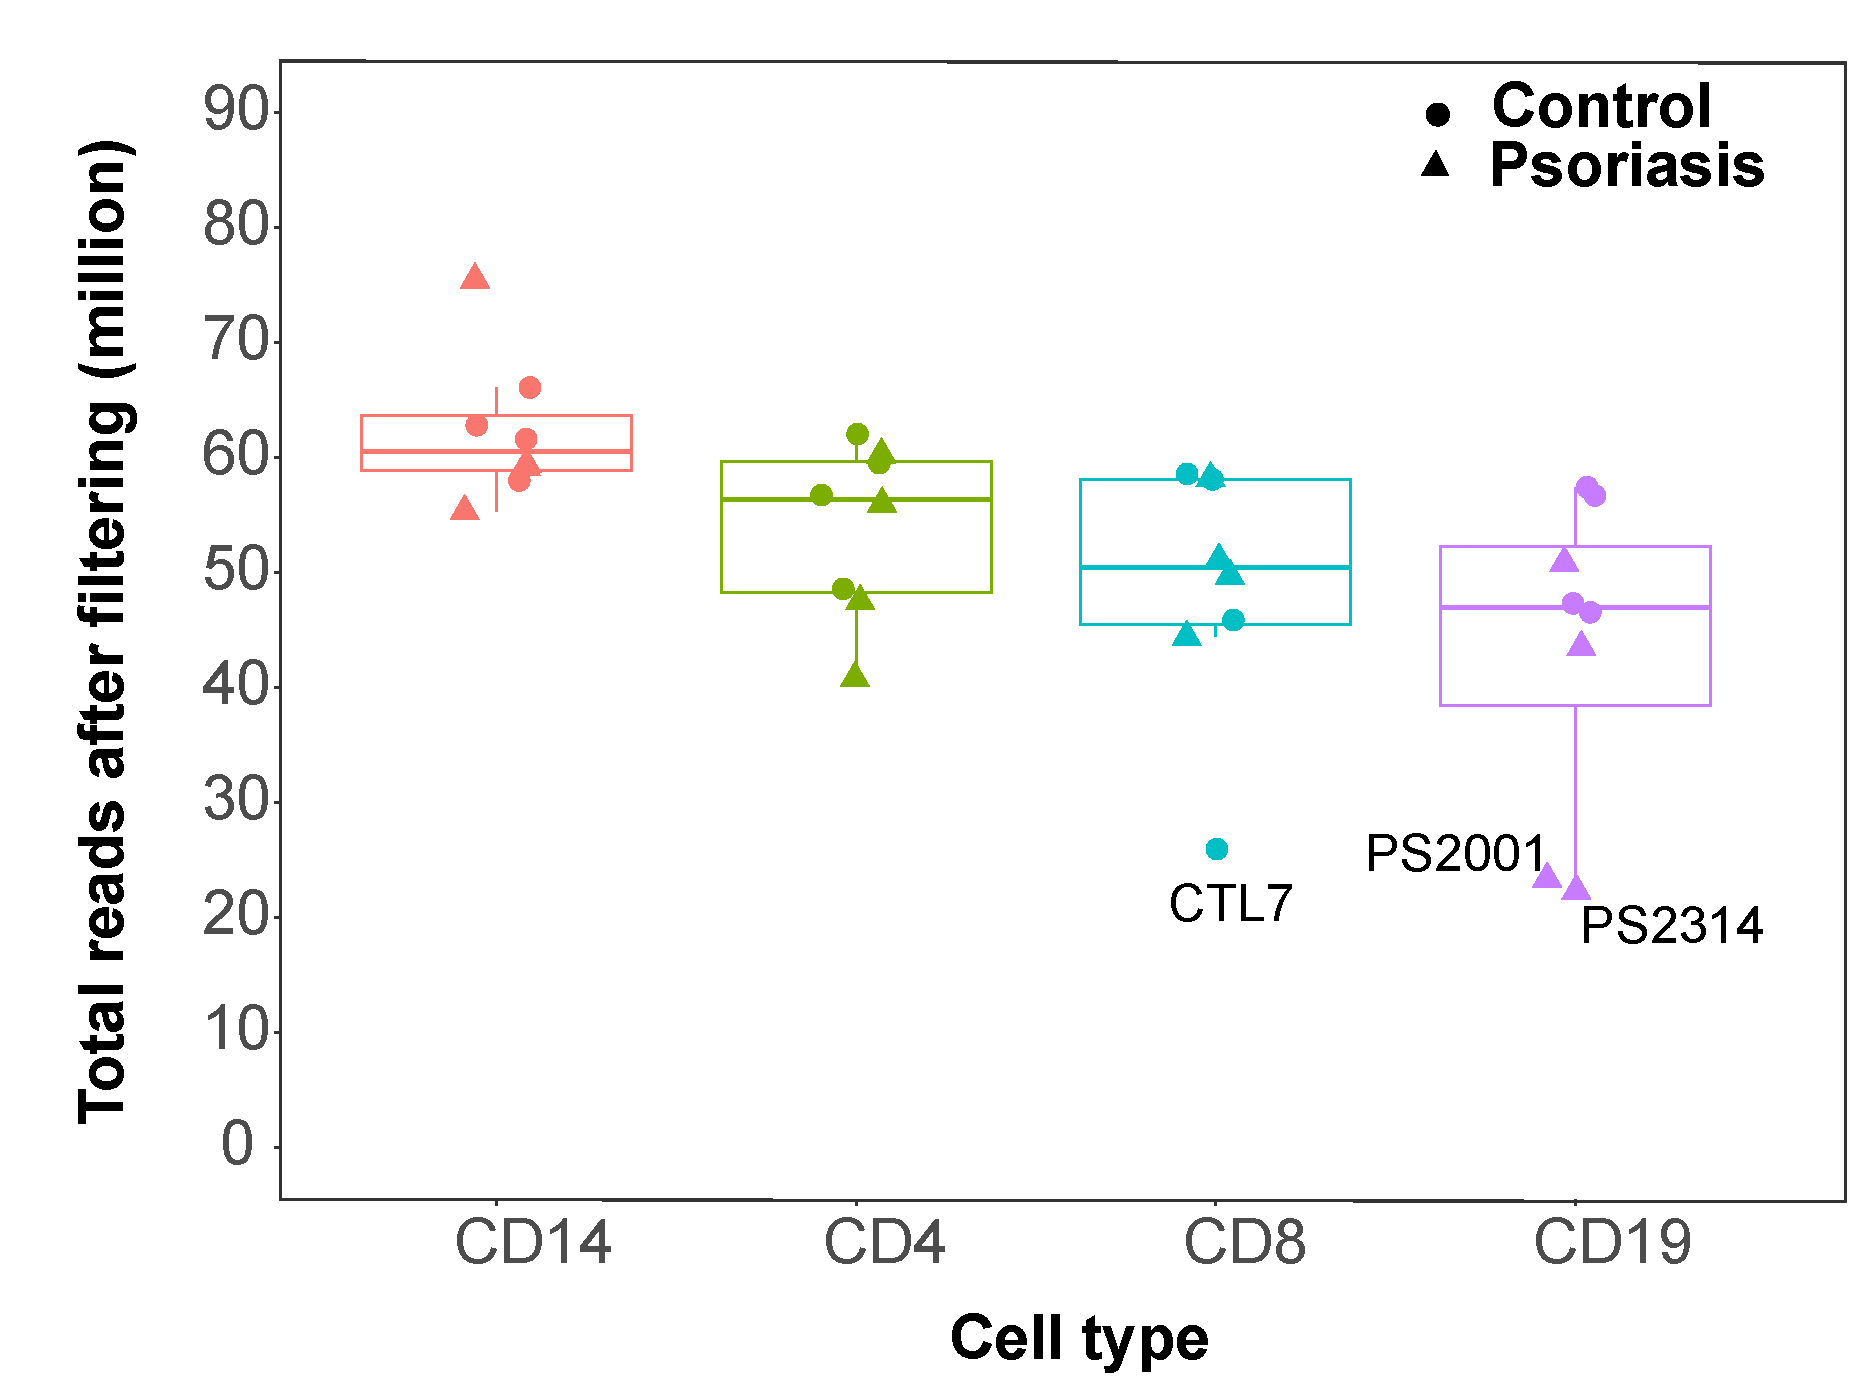
\includegraphics[width=\textwidth]{./Results2/pdfs/ChIPm_PS_CTL_final_filtered_reads_boxplot}
\caption{\textbf{}}
% The percentage sign indicated that the other subfig goes side by side
\end{subfigure} \\
\begin{subfigure}{0.5\textwidth}
\centering
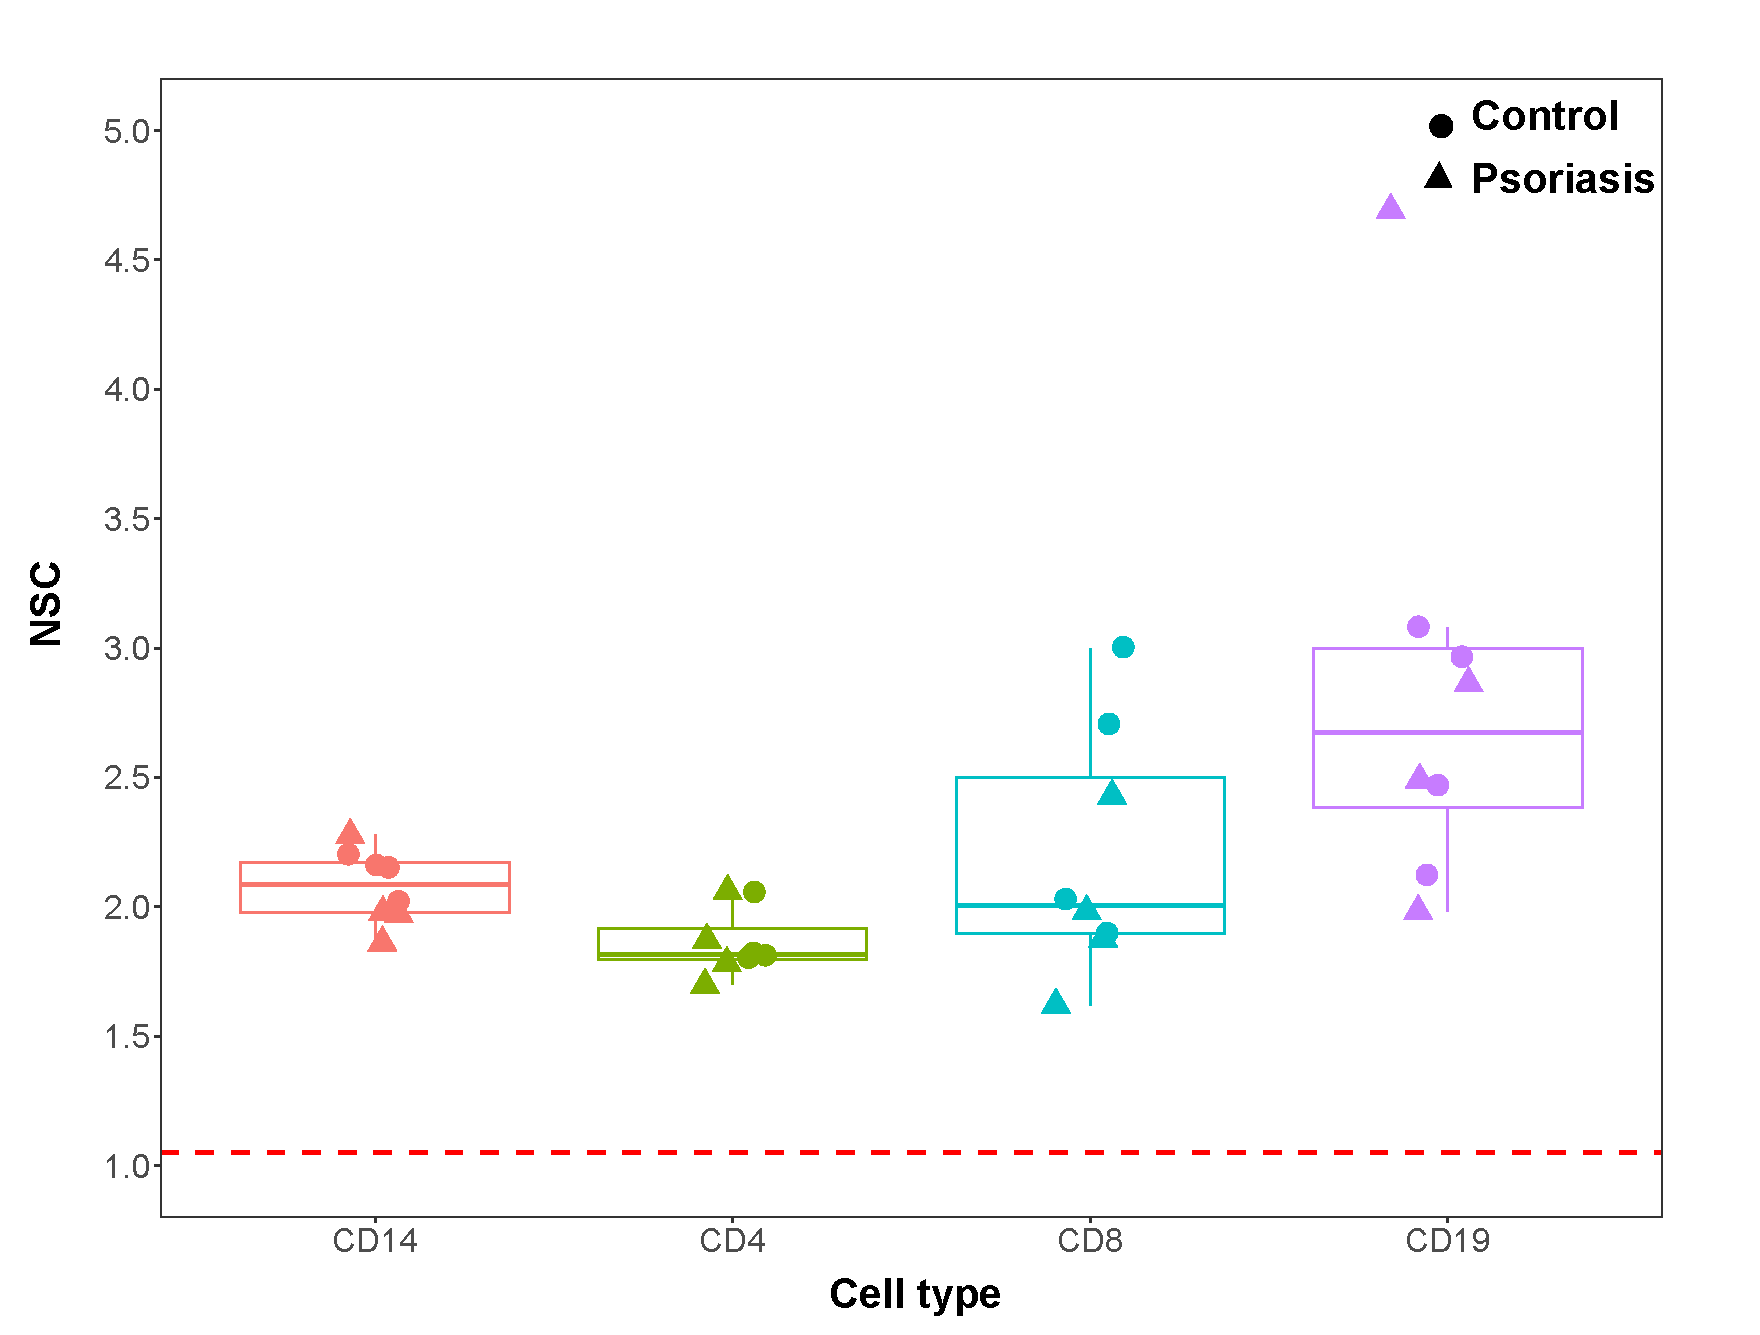
\includegraphics[width=\textwidth]{./Results2/pdfs/ChIPm_PS_CTL_NSC_boxplot}
\caption{\textbf{}}
\end{subfigure}%
\begin{subfigure}{0.5\textwidth}
\centering
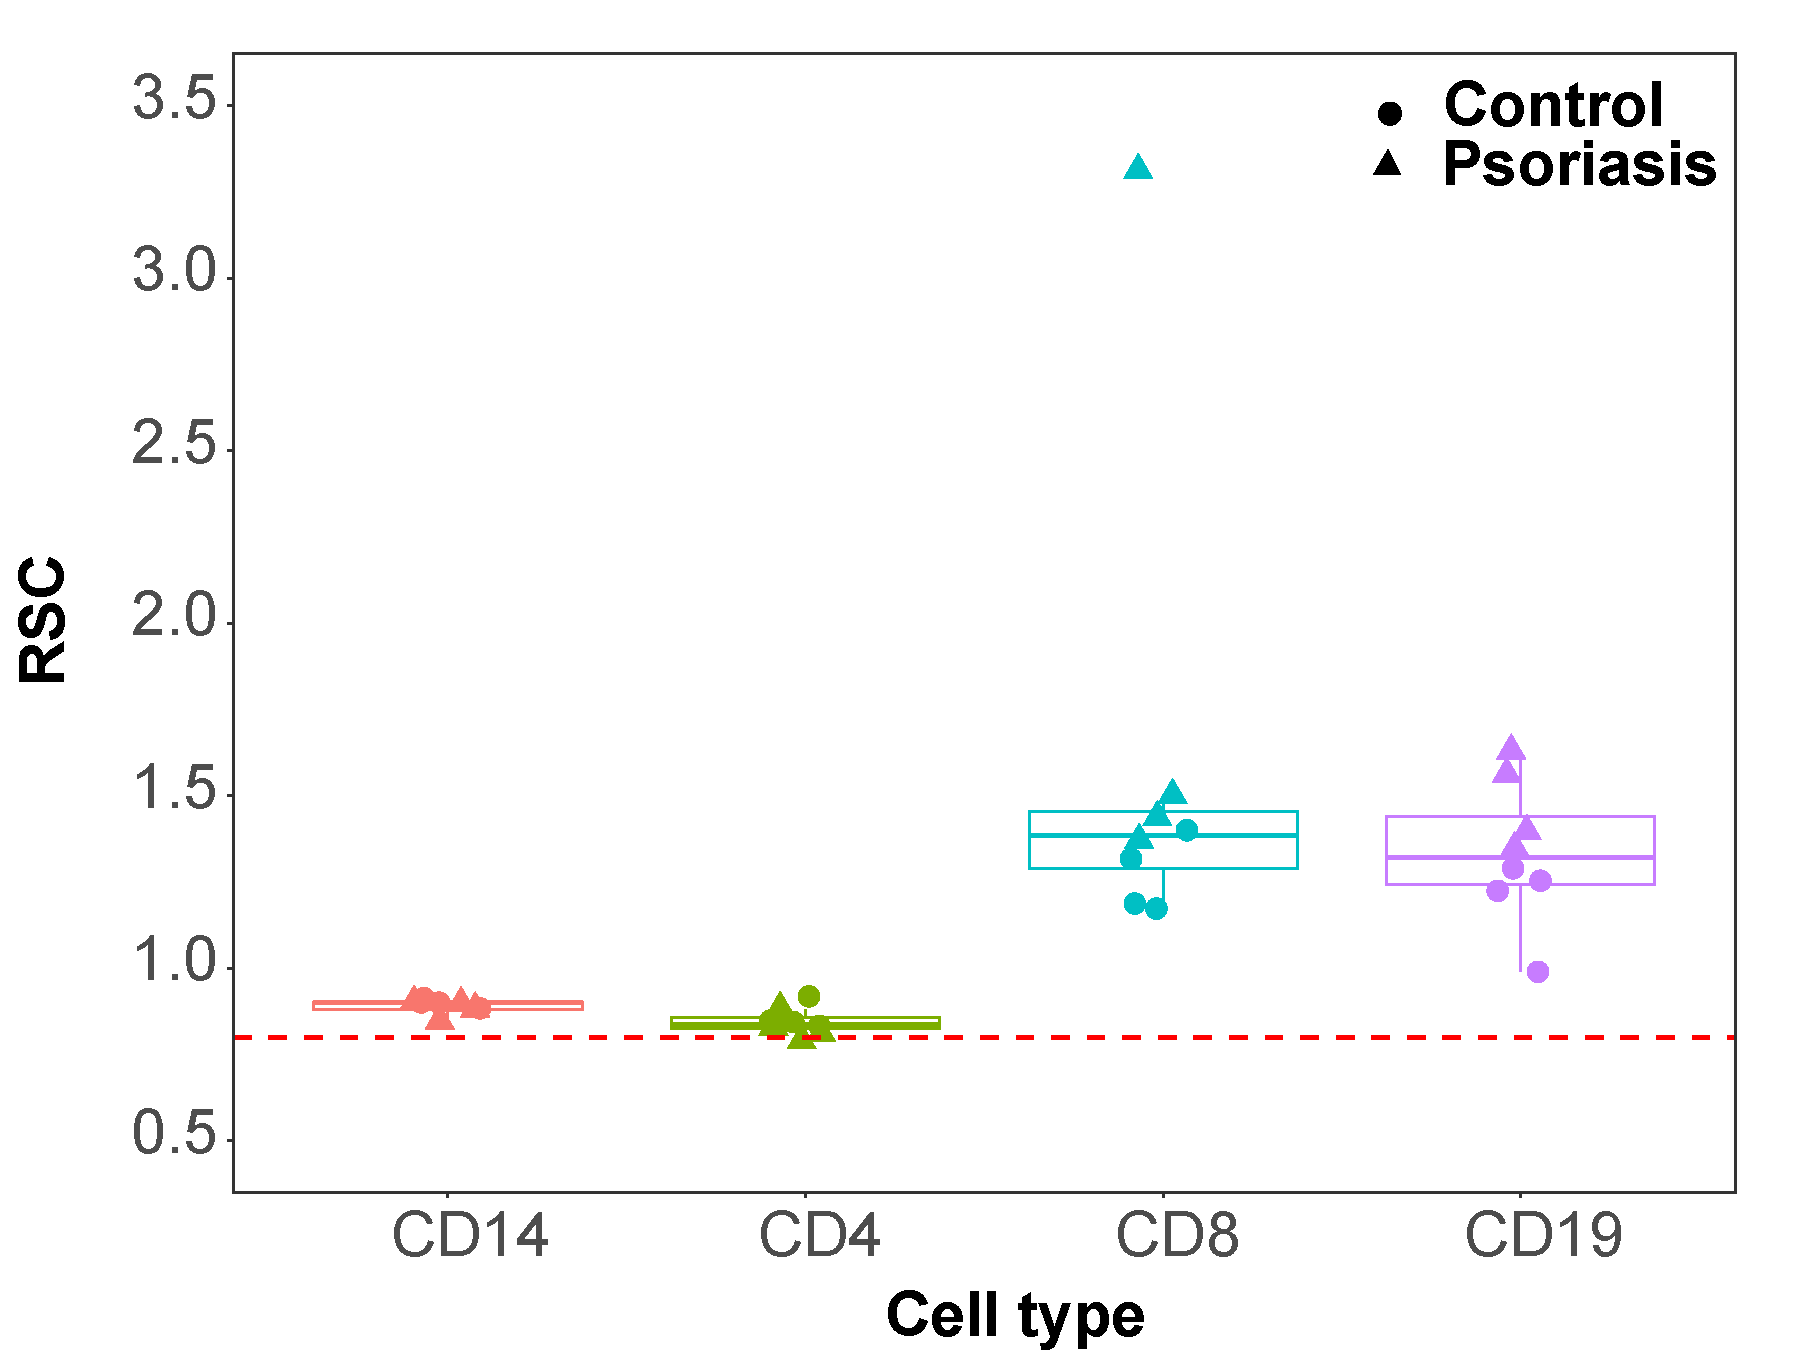
\includegraphics[width=\textwidth]{./Results2/pdfs/ChIPm_PS_CTL_RSC_boxplot}
\caption{\textbf{}}
\end{subfigure}
\caption[Quality control evaluation of the H3K27ac ChIPm libraries in immune cells isolated from psoriasis and control samples.]{\textbf{Quality control evaluation of the H3K27ac ChIPm libraries in immune cells isolated from psoriasis and control samples.}}
\label{figure:ChIPm_PS_CTL_QC}
\end{figure} 

PCA analysis using a combined master list of the H3K27ac enriched sites in patients and controls for all four cell types (excluding the aforementioned low quality samples) confirmed the ability of this data to recapitulate the cell type specific epigenetic landscape of this enhancer mark and reinforced the appropriate quality of the data (Figure \ref{figure:ChIPm_PCA_and_chromatin_states} a). When performing PCA analysis by cell type, the PS2314 CD8$^+$ library appeared as an outlier compared to the rest of CD8$^+$ H3K27ac ChIPm patients and control libraries and was also removed for downstream analysis (data not shown). 

\bigskip
\begin{figure}[H]
\centering
\begin{subfigure}[b]{0.6\textwidth}
\centering 
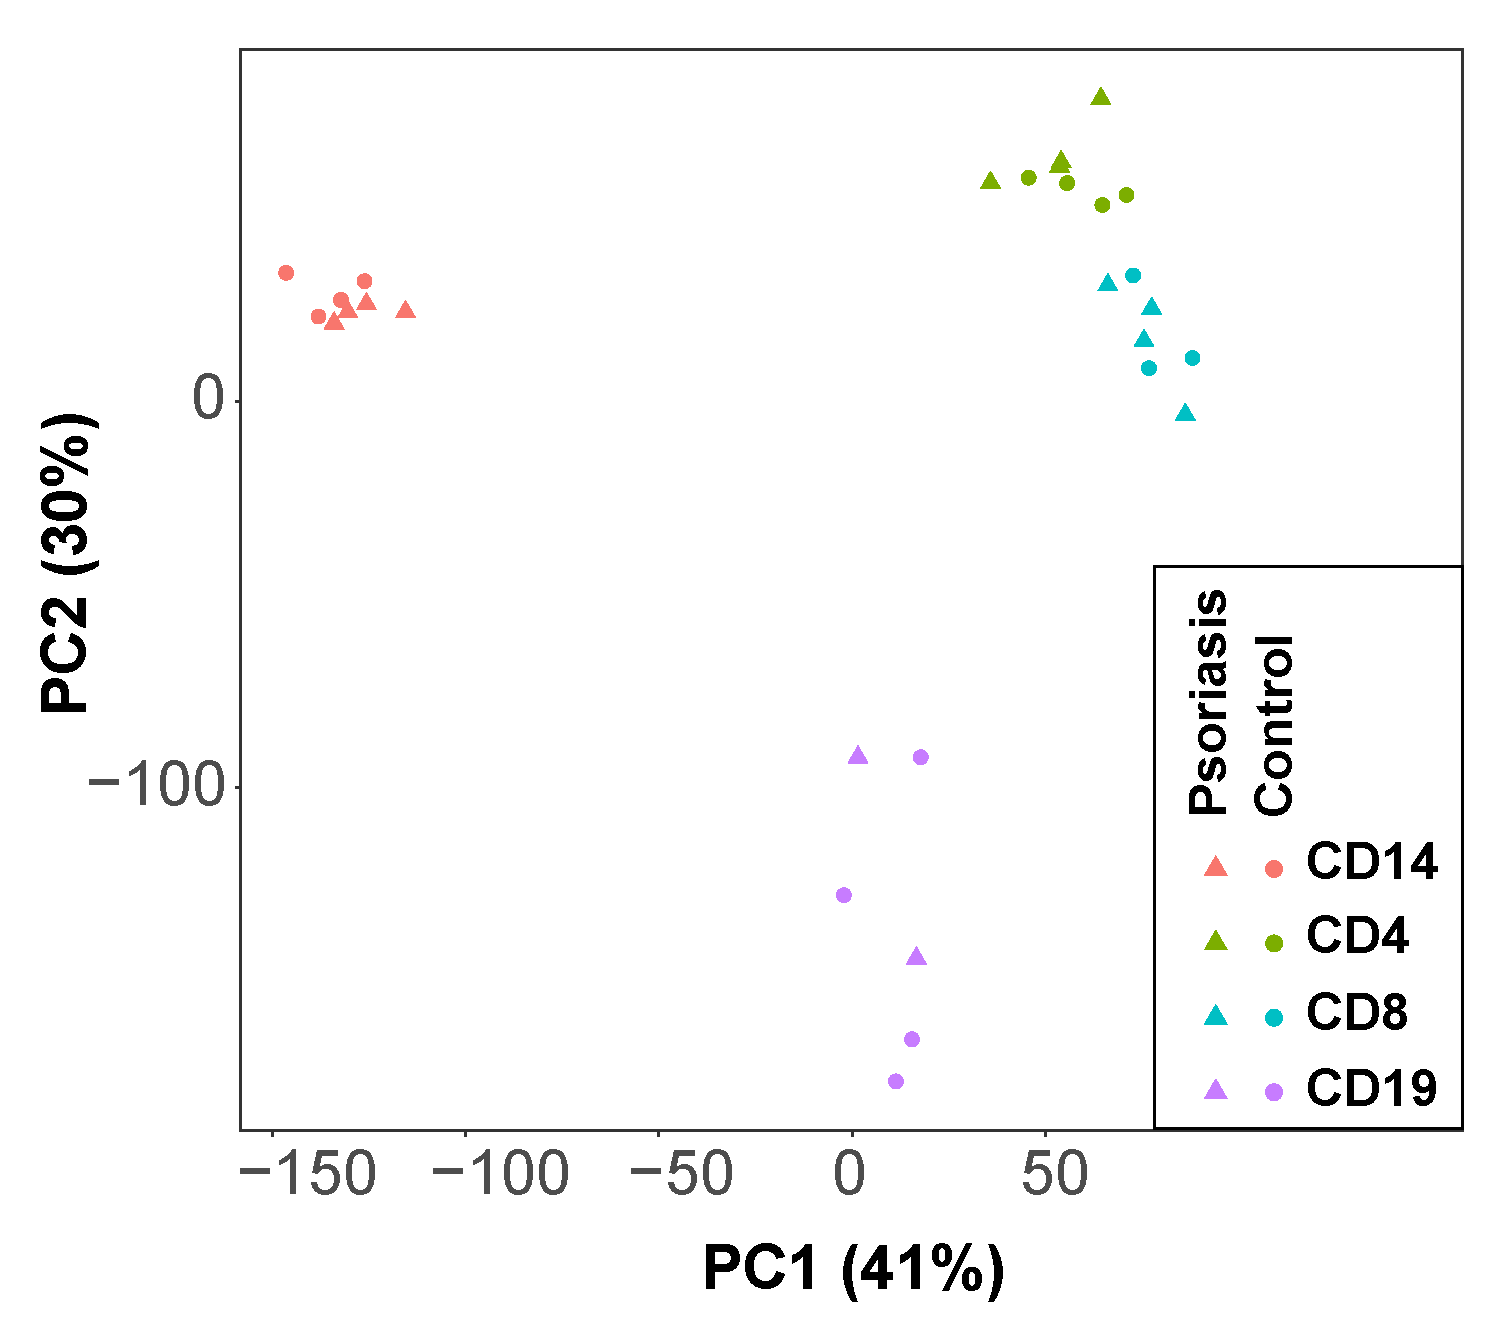
\includegraphics[width=\textwidth]{./Results2/pdfs/ChIPm_H3K27ac_all_cell_types_filtered_PCA}
\caption{}
\end{subfigure}
~
\begin{subfigure}[b]{0.8\textwidth} 
%the [b] prevents offset in subcaptions
\centering
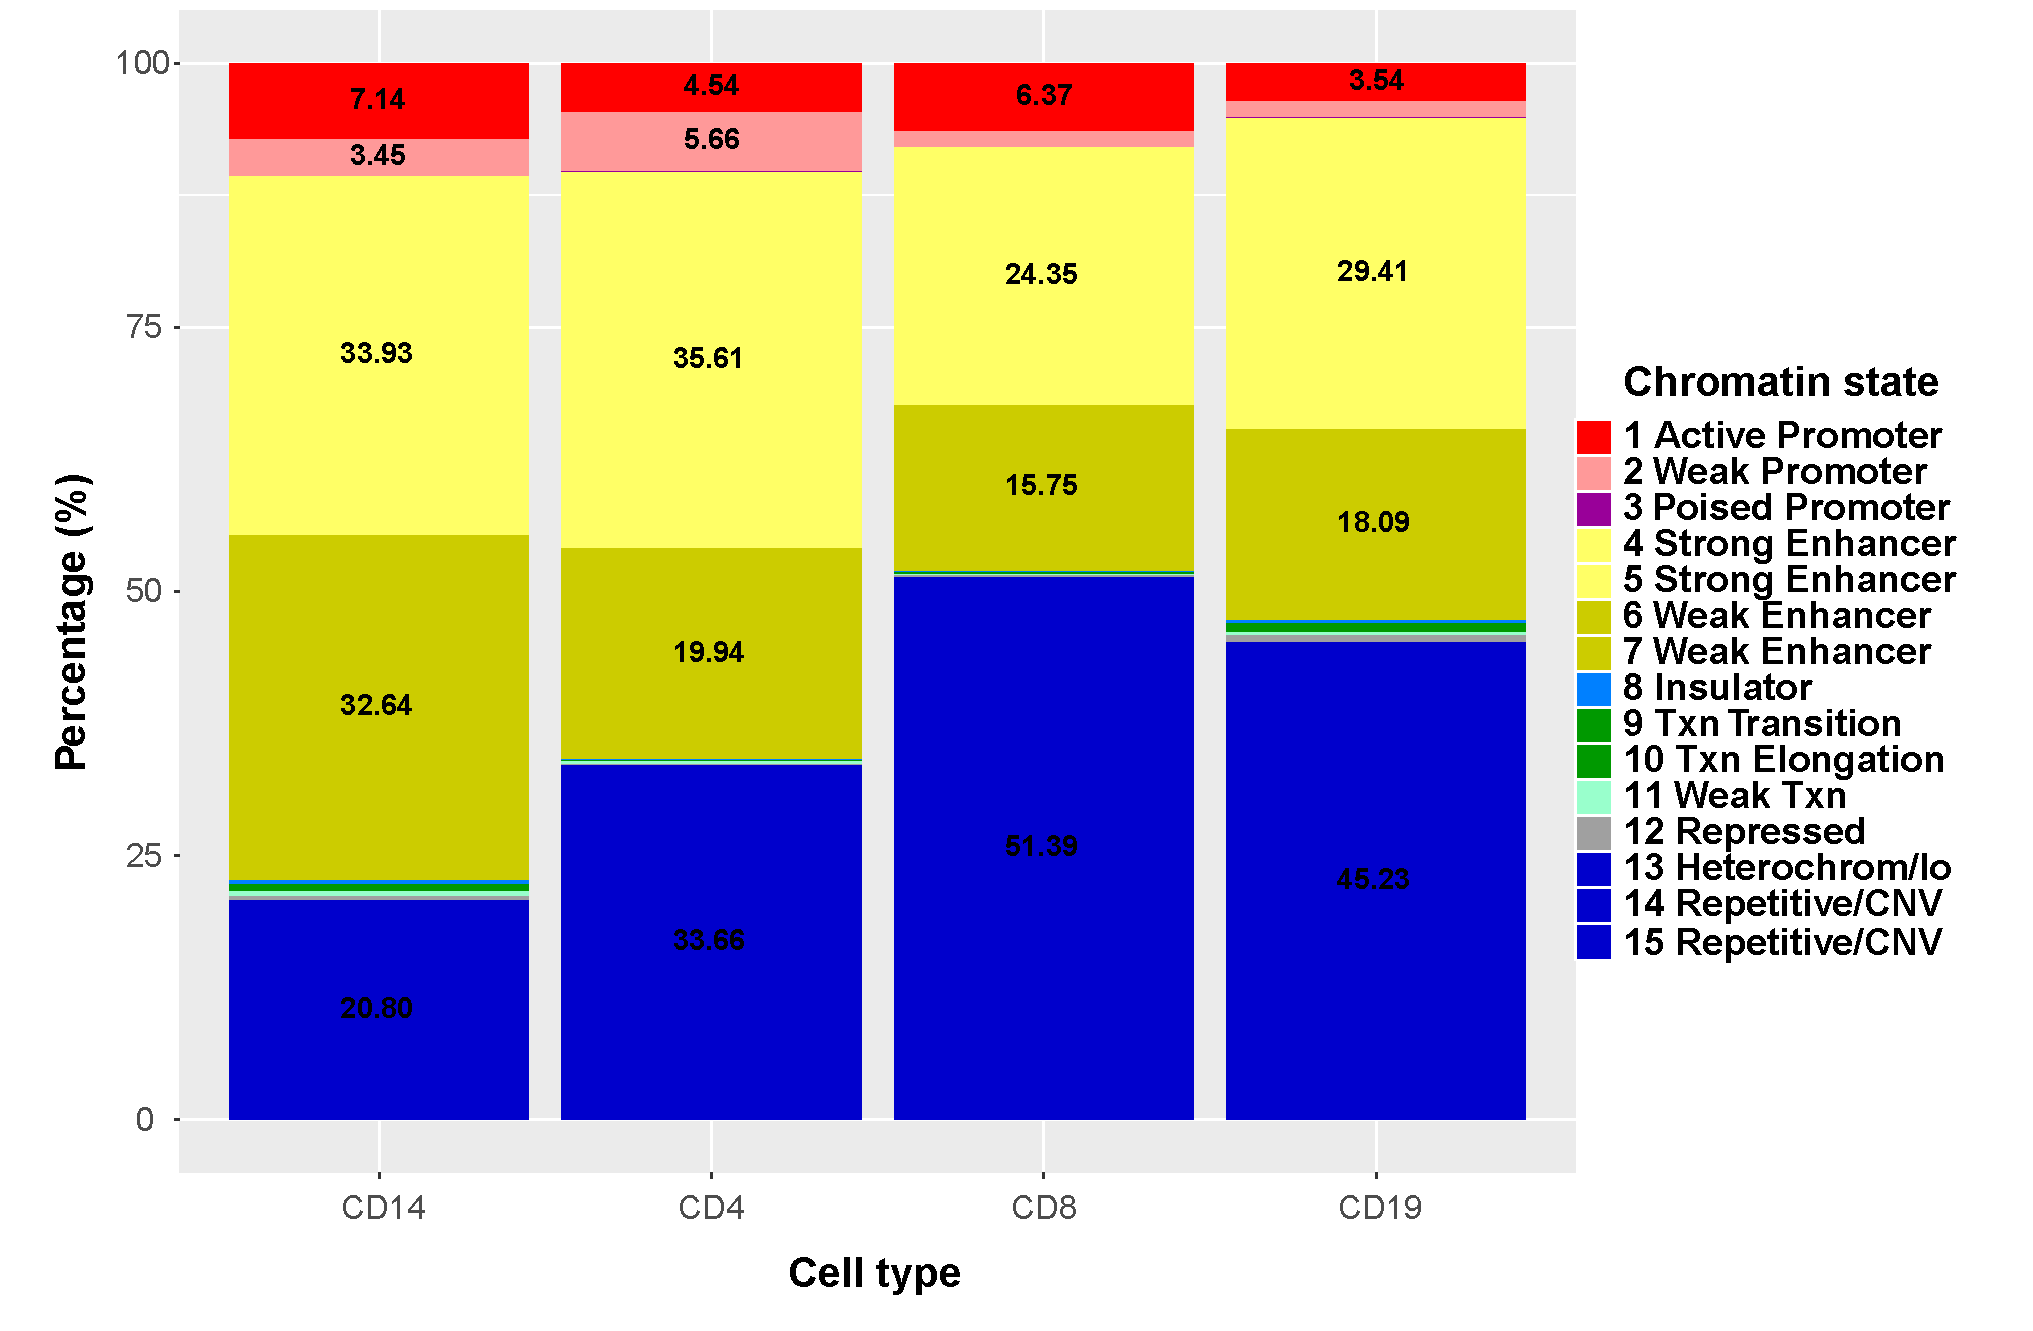
\includegraphics[width=\textwidth]{./Results2/pdfs/ChIPm_H3K27ac_cell_type_specific_master_list_chromatin_states_annotated_filtered}
\caption{}
\end{subfigure}
\caption[PCA analysis and chromatin annotation states of the H3K27ac enriched sites in four immune primary cell types from psoriasis and healthy control samples.]{\textbf{PCA analysis and chromatin annotation states of the H3K27ac enriched sites in four immune primary cell types from psoriasis and healthy control samples.} a) PCA analysis was performed using the normalised counts across a consensus master list of the combined H3K27ac enriched regions in psoriasis patients and healthy control samples across CD14$^+$ monocytes, CD4$^+$, CD8$^+$ and CD19$^+$ cells. b) Annotation of the H3K27ac list of consensus enriched sites built by DiffBind for each cell was performed using the appropriate cell type specific RoadMap chromatin segmentation maps. Results are expressed as the percentage of regions annotated with a particular chromatin state over the total number of H3K27ac enriched sites in each of the four cell type master lists.}
\label{figure:ChIPm_PCA_and_chromatin_states}
\end{figure}



Differential analysis for H3K27ac was performed for each cell type between psoriasis and healthy control samples using DiffBind. The consensus merged list of H3K27ac sites assembled by this algorithm to perform the differential analysis (as explained in Chapter \ref{ch:Mat}) showed a great percentage of those sites to be annotated as heterochromatin or repetitive (Figure \ref{figure:ChIPm_PCA_and_chromatin_states} b). These percentages ranged from 20.8 to 51.39\% in CD14$^+$ monocytes and total CD8$^+$ cells, respectively, which are less likely to be relevant since H3K27ac is a histone modification mainly enriched at enhancers. When restricting the differential analysis to those regions annotated as enhancers (weak and strong), CD14$^+$ monocytes appeared as the cell type with the greatest number of differentially modified enhancers (8 hits), followed by CD4$^+$ (4 hits) and CD8$^+$ (1 hit) (Table \ref{tab:ChIPm_differential_analysis_results}).



\begin{table}[htbp]
%\setlength{\tabcolsep}{20pt} only to stretch the columns if you want
%\renewcommand{\arraystretch}{1.5}
\centering
\begin{tabular}{@{} c c c}
\toprule
\textbf{Cell type}   & \textbf{Master list size}      & \textbf{Differential regions}      \\
                     & \textbf{genome-wide/enhancers} & \textbf{genome-wide/enhancers}     \\
\midrule
\midrule
CD14$^+$             & 99,862/60,962                  & 15/8                                \\
CD4$^+$              & 110,353/56,282                 & 0/4																	\\
CD8$^+$              & 137,194/51,607                 & 8/1                                 \\ 
CD19$^+$             & 199,014/88,722                 & 12/0                                 \\
\bottomrule 
\end{tabular}
\medskip %gap
\caption[Summary results from the differential H3K27ac analysis between psoriasis patients and healthy controls in CD14$^+$ monocytes, CD4$^+$, CD8$^+$ and CD19$^+$ cells.]{\textbf{Summary results from the differential H3K27ac analysis between psoriasis patients and healthy controls in CD14$^+$ monocytes, CD4$^+$, CD8$^+$ and CD19$^+$ cells.} In the genome-wide analysis, the master list size refers to the number of H3K27ac enriched sites included in the consensus list built by DiffBind to perform the differential analysis. In the analysis restricted to enhancers, the size of the master list was reduced to only those sites from the genome-wide master list annotated as enhancers (weak and strong) according to the chromatin segmentation map for each particular cell type. Genome-wide hits in CD14$^+$ monocytes and CD8$^+$ also contained the hits identified in the enhancers restricted analysis. Significant differentially H3K27ac regions using FDR$<$0.05 and no FC threshold. }
\label{tab:ChIPm_differential_analysis_results}
\end{table}
\bigskip %bigger space


One of the differentially acetylated regions between patients and controls in CD14$^+$ monocytes is at an enhancer located between the 3' UTR of the genes \textit{SLC15A2} and \textit{ILDR2} (Figure \ref{figure:ChIPm_H3K27ac_UCSC_ILDR1_track}). Consistently with its annotation as an enhancer, this region is overlapping a DHS site and H3Kme1 (enhancer mark) modifications. Although \textit{ILDR2} is widely expressed in immune cells and has recently been proven to act as a negative regulator for T cells, publicly available promoter capture and Hi-C data failed to show interactions of this regions with the promoter of any gene. Conversely, this region harbours SNPs that have been identified as \textit{cis}-eQTL in whole blood and total unstimulated and stimulated CD14$^+$ monocytes for the calmodulin-binding motif-containing protein \textit{IQCB1} gene, at 186.4Kb up-stream this peak \parencite{GTeX,Fairfax2014}. MS risk LD SNPs (rs34543553, rs73855480 and rs73855480) in this peak are also \textit{cis}-eQTLs in unstimulated total CD4$^+$ and CD8$^+$ cells for \textit{IQCB1} \parencite{Kasela2017}, which has been prioritised by Dr Fang in-house pipeline as a potential drug target for this autoimmune disease. Amongst the CD4$^+$ hits, all the regions presented very moderated changes with no evidence of regulating expression of any relevant gene.

*CTCF peak may help to maintain, edit to K562 or remove

\begin{figure}[htbp]
\centering
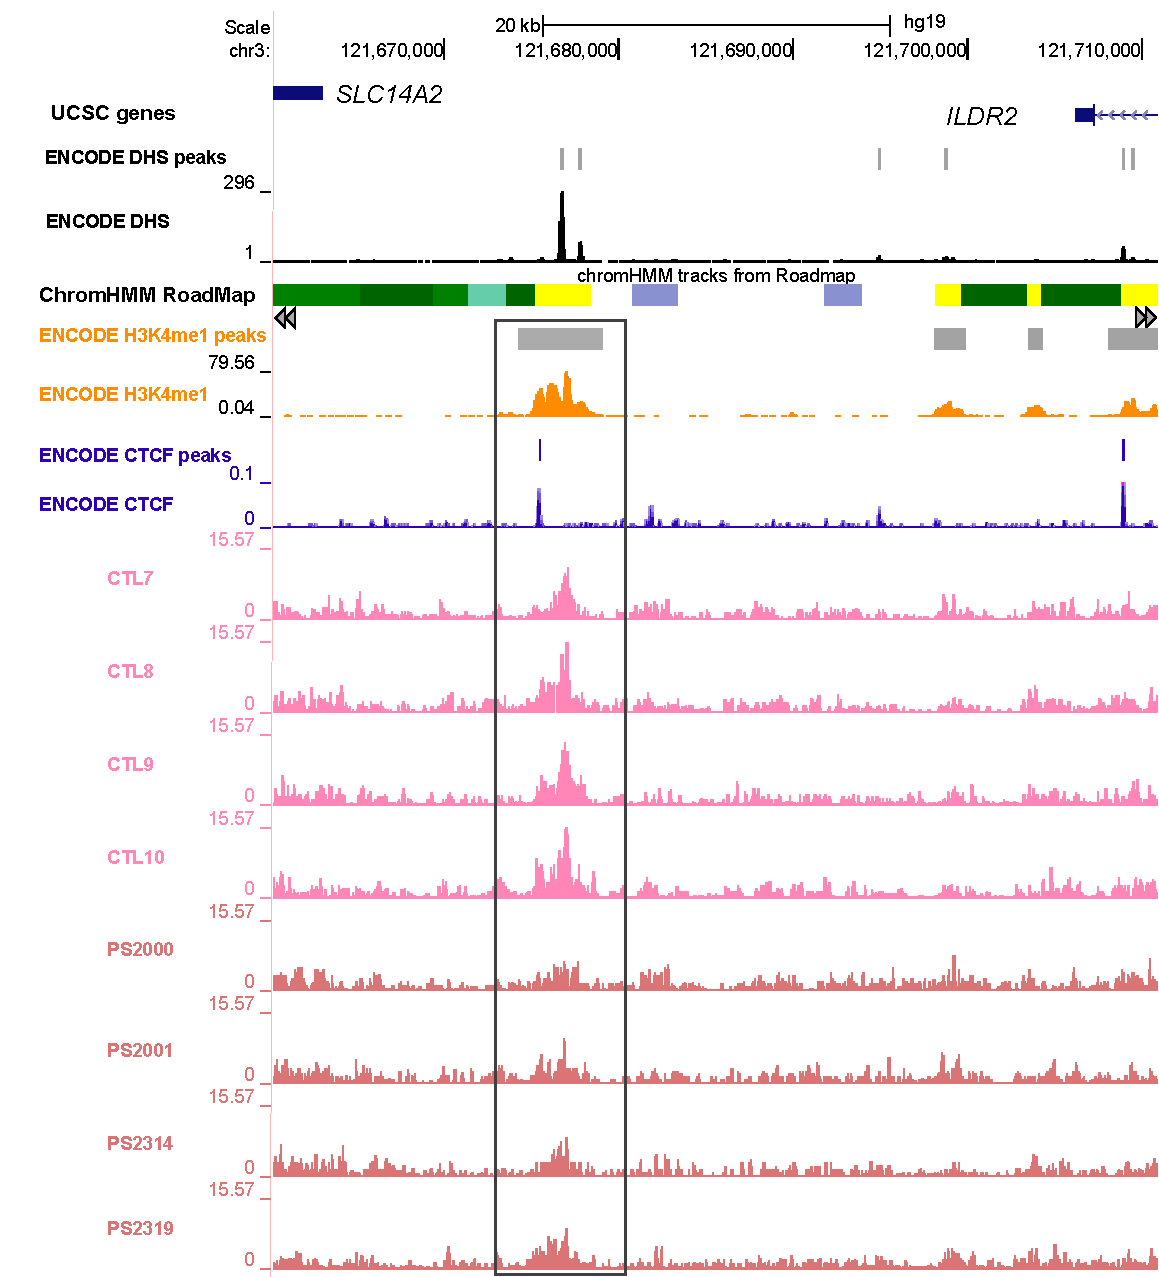
\includegraphics[width=0.6\textwidth]{./Results2/pdfs/ChIPm_H3K27ac_UCSC_CD14_ILDR1_track}
\caption[Epigenetic landscape at the chr3:121,675,048-121,677,505 enhancer in circulating CD14$^+$ monocytes from psoriasis patients and healthy controls.]{\textbf{Epigenetic accessibility landscape at the chr3:121,675,048-121,677,505 enhancer in circulating CD14$^+$ monocytes from psoriasis patients and healthy controls.} Describe the track }
\label{figure:ChIPm_H3K27ac_UCSC_ILDR1_track}
\end{figure}



When performing genome-wide differential analysis, CD14$^+$ monocytes and CD8$^+$ revealed additional statistically significant differentially H3K27ac modified regions, which also included those already identified in the restricted enhancers analysis (Table \ref{tab:ChIPm_differential_analysis_results}). The newly identified regions in both cell types were mostly in regions lacking of ATAC-seq and H3K4me1 signal or interactions with nearby gene regulatory regions. Genome-wide analysis in CD4$^+$ cells did not identify significant differentially modified targets outside enhancers and also failed to retain significance for the four hits identified in the restricted analysis, most likely due to increase in multiple testing due to the increase in size of the master list (Table \ref{tab:ChIPm_differential_analysis_results}). Interestingly, the differential regions between psoriasis patients and controls identified in CD19$^+$ cells when performing genome-wide analysis presented considerable fold changes (absolute log$_2$FC ranging from 2.47 to 6.37). However, most of them (10out of 12) did not overlap open chromatin regions and none was found to be interacting with other enhancers or distal promoters. The absence of differentially H3K27ac sites between patients and controls at CD19$^+$ enhancers may be reinforcing the lack of relevance of circulating B cells in psoriasis when compared to the other three cell types.

Overall, restricting the differential analysis to enhancer annotated regions did not show a great increase in the number of significant differentially modified H3K27ac sites when compared to the genome-wide analysis in any of the four cell types. The results in this pilot cohort did not show relevant global epigenetic changes in H3K27ac sites between psoriasis patients and controls at the systemic level for these cell types and sample size.


\subsubsection{Identifying global changes in immune cells chromatin accessibility between psoriasis patients and healthy controls}

As previously explained, the cell type specific chromatin accessibility landscape is determined by the the combination of histone modifications and DNA binding proteins (including TF and co-regulatory proteins) in a particular locus. The previous results showing only moderate changes in the H3K27ac landscape between patients and controls are not necessarily representative of the overall changes in the chromatin accessibility landscape in disease. In order to interrogate genome-wide changes in chromatin accessibility between patients and controls not restricted to changes in H3K27ac, ATAC-seq was performed in the same four cell types in 8 patients and 10 controls (Table \ref{tab:Psoriasis_controls_datasets_per_sample})

ATAC-seq quality control was performed in 72 libraries generated in CD14$^+$ monocytes, total CD4$^+$, total CD8$^+$ and CD19$^+$ cells from psoriasis patients and control individuals. The median of total reads after filtering ranged between 39.2 and 49.8 in CD4$^+$ and CD19$^+$ ,respectively, and was over the 15 million reads determined as appropriate minimum (Chapter \ref{ch:Results1}) in all the samples (Figure \ref{figure:ATAC_PS_CTL_QC} a). 



\begin{figure}[htbp]
\centering
\begin{subfigure}{0.5\textwidth}
\centering
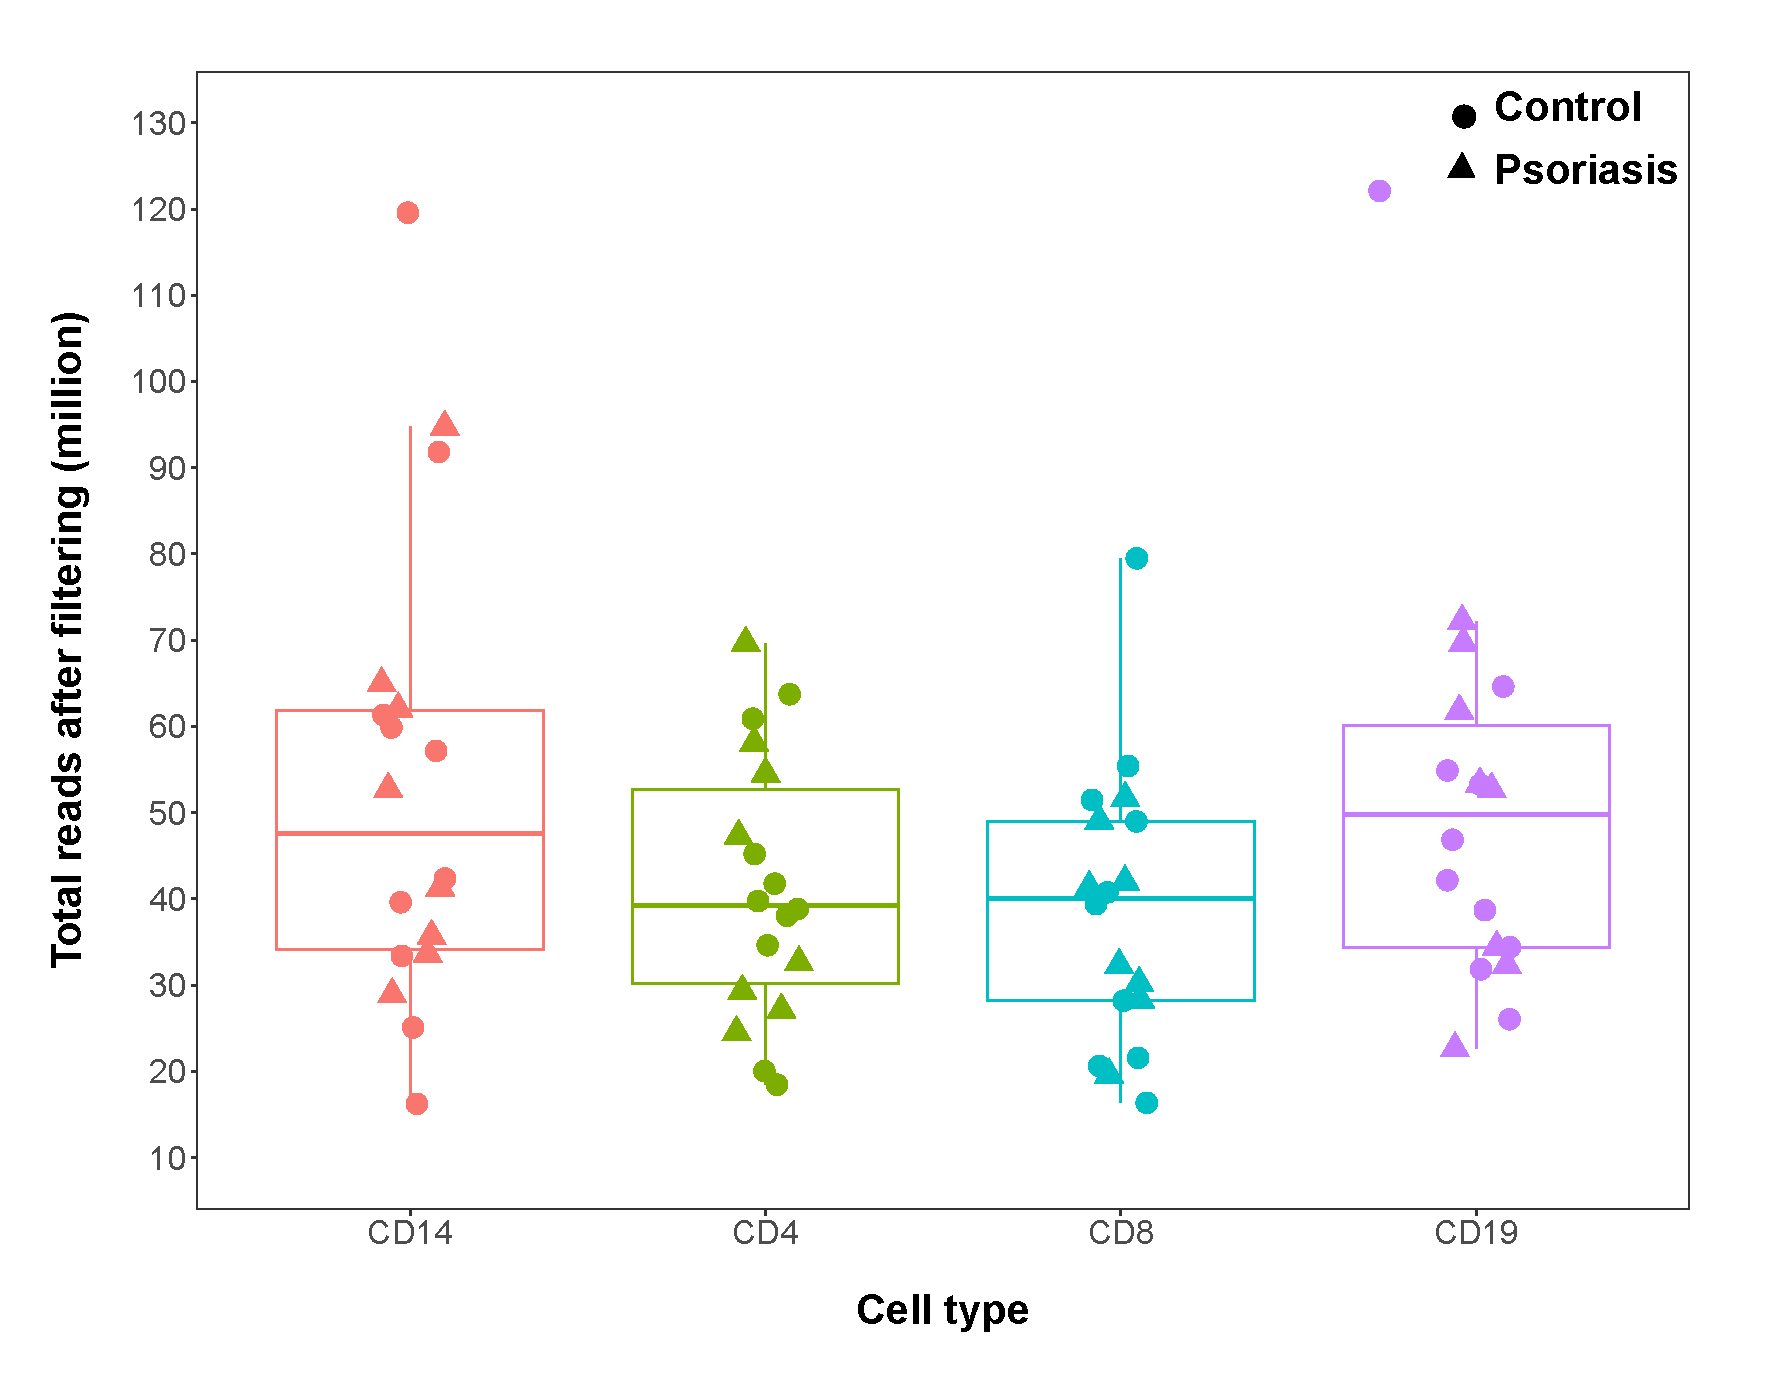
\includegraphics[width=\textwidth]{./Results2/pdfs/ATAC_PS_CTL_final_filtered_reads_boxplot}
\caption{\textbf{}}
% The percentage sign indicated that the other subfig goes side by side
\end{subfigure}%
\begin{subfigure}{0.5\textwidth}
\centering
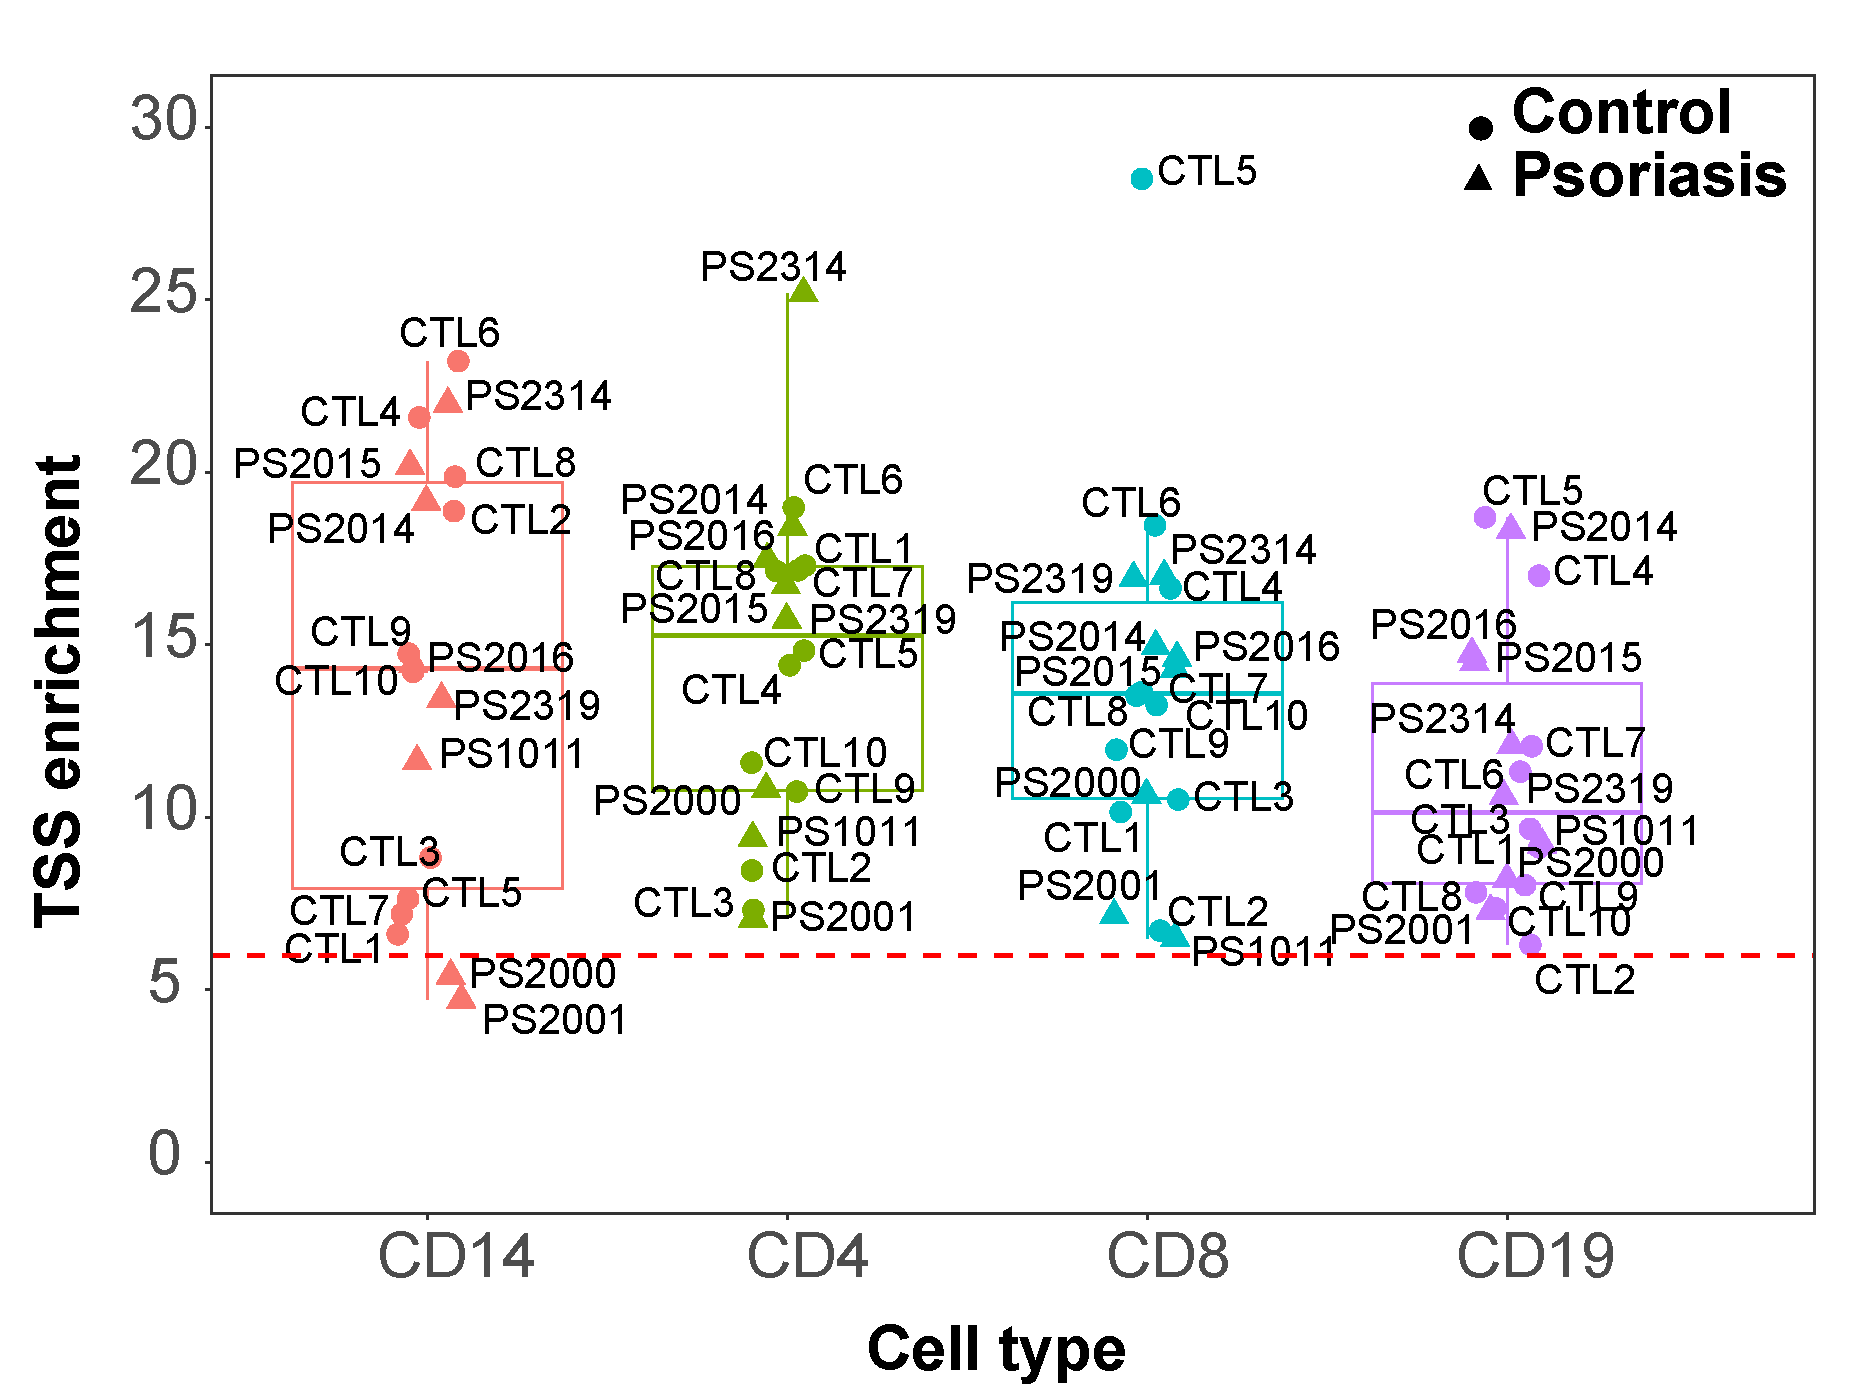
\includegraphics[width=\textwidth]{./Results2/pdfs/ATAC_PS_CTL_all_samples_TSS_boxplots_all_labelled}
\caption{\textbf{}}
\end{subfigure}
\begin{subfigure}{0.5\textwidth}
\centering
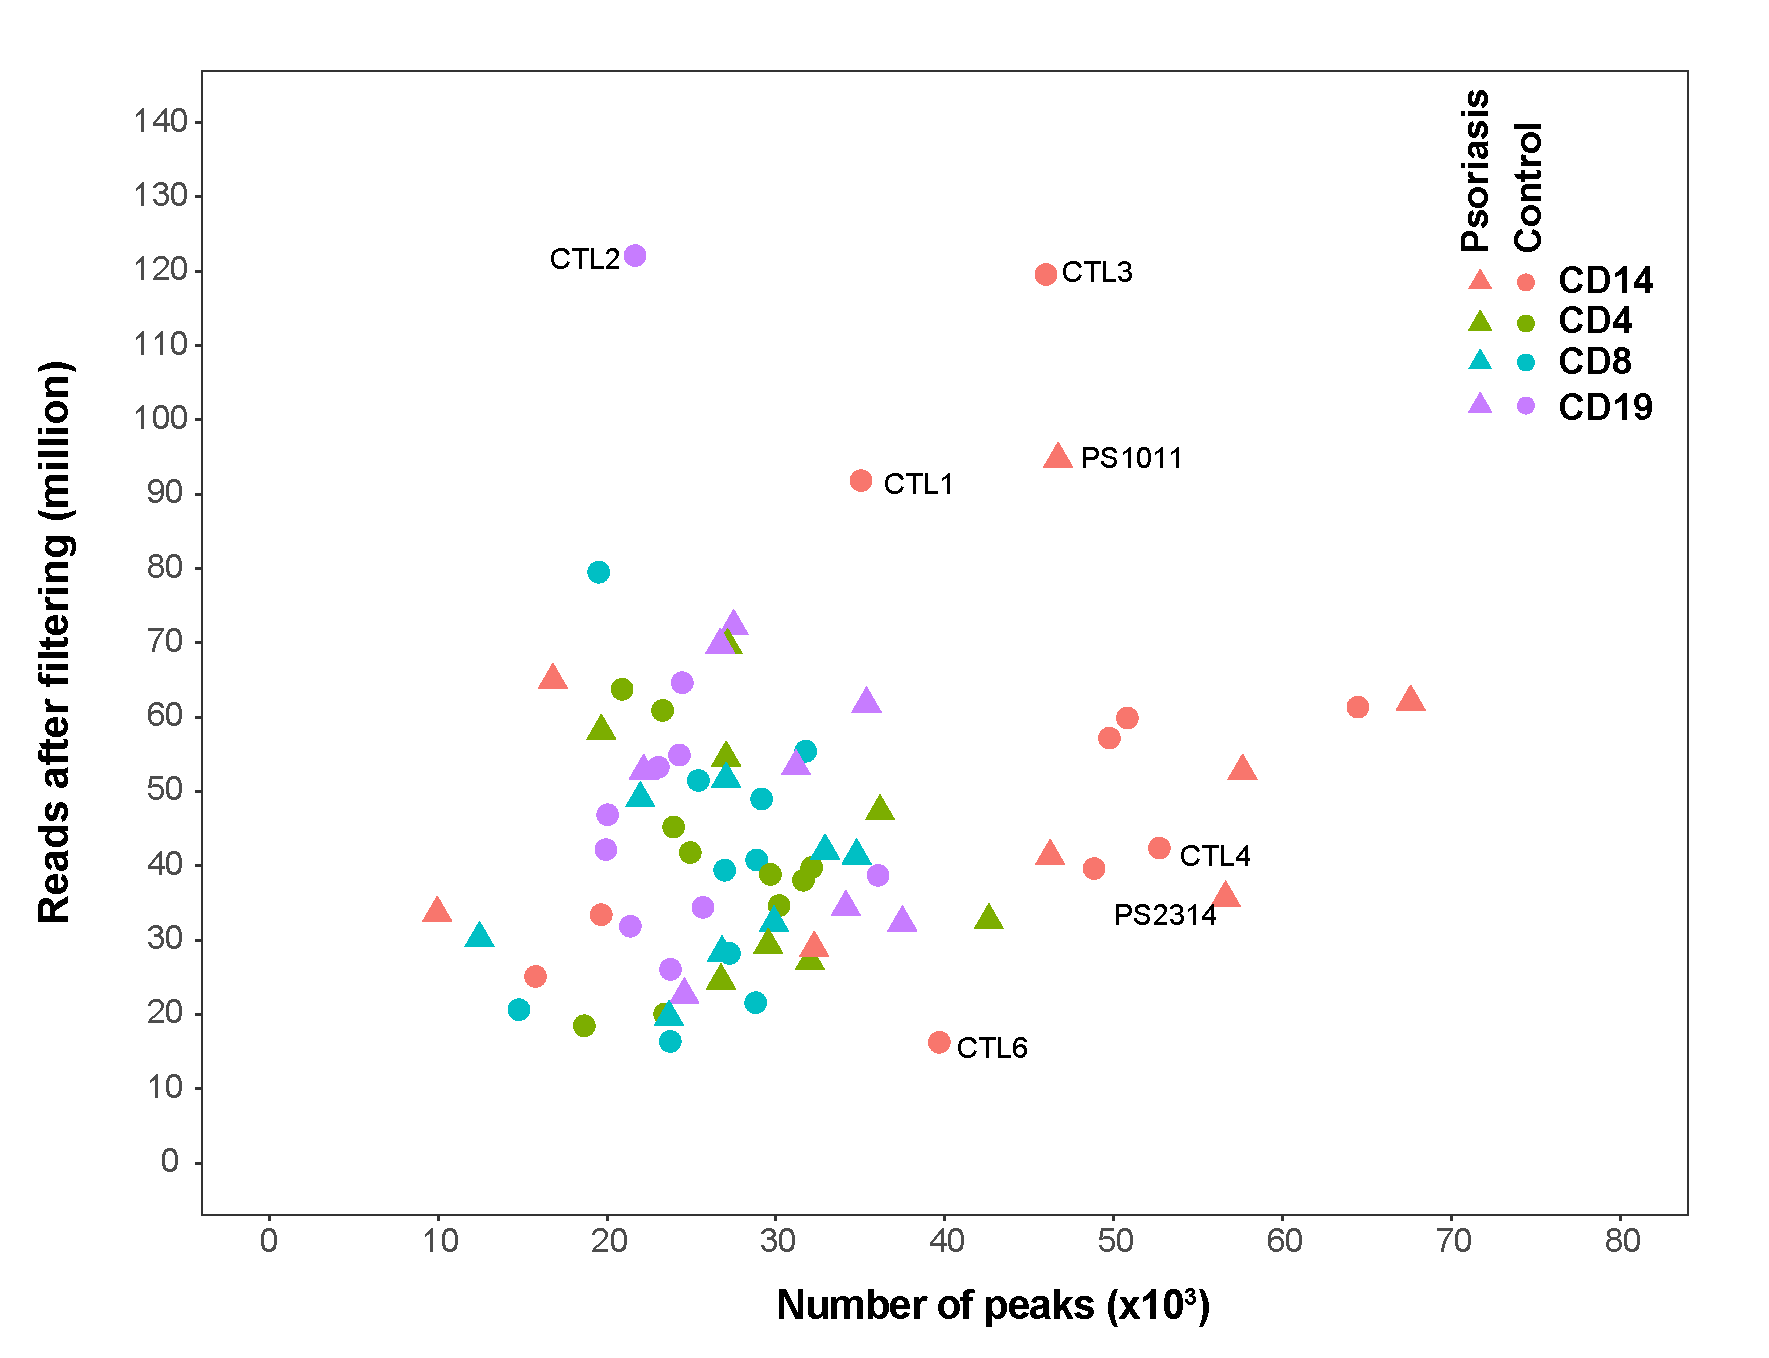
\includegraphics[width=\textwidth]{./Results2/pdfs/ATAC_PS_CTL_reads_vs_peaks_dotplot}
\caption{\textbf{}}
\end{subfigure}
\caption[Quality control assessment of the ATAC-seq libraries generated from immune cells in psoriasis and control samples.]{\textbf{Quality control assessment of the ATAC-seq libraries generated from immune cells in psoriasis and control samples.}xxx}
\label{figure:ATAC_PS_CTL_QC}
\end{figure} 


The differences in read depths across ATAC-seq samples are mostly due to the difficulties in appropriate determining the molarity of the libraries prior to the sequencing pooling (due to the fragment size heterogeneity) as well as the number of duplicates present in each library, which also correlated with MT reads, as previously mentioned. In this particular case, differences in the percentage of MT reads were observed between samples from cohort 1A generated with standard ATAC-seq protocol from Buenrostro \textit{et al.}, 2013 and the FAST-ATAC libraries of cohort 1B using the later modified \parencite{Corces2016} protocol (Figure \ref{figure:ATAC_PS_CTL_MT_percent}). 

All the samples presented the characteristic ATAC-seq fragment size distribution recapitulating nucleosome periodicity, which is one of the measured to determine samples quality control, as previously detailed in Chapter \ref{ch:Results1} (data not shown). Analysis of ATAC-seq signal enrichment across gene TSS revealed that most of the samples had enrichment over 6, considered the lower threshold by ENCODE (Figure \ref{figure:ATAC_PS_CTL_QC} b) and only PS2000 and PS2001 CD14$+$ monocytes were removed from downstream analysis due to low signal-to-noise ratios. When comparing the number of peaks passing IDR filtering in each samples versus the number of reads after filtering, most of the samples presented between 10,000 to 35,000 peaks (Figure \ref{figure:ATAC_PS_CTL_QC} c). Since sequencing depth of most of the samples was equal or greater than 15 million reads, most of the differences in number of called peaks were intrinsic to the cell type and the signal-to-noise differences in the samples, as previously studied in Chapter \ref{ch:Results1}. For example, CD14$^+$ monocytes presented greater number of peaks when compared to the other three cell types, despite the median of total number of reads after filtering being similar to the other cell types (Figure \ref{figure:ATAC_PS_CTL_QC} a). Also, within the CD14$^+$ monocytes samples, those with the greatest TSS fold-enrichment (e.g CTL4, CTL6 and PS2314) presented similar number of good quality called peaks to the samples with higher number of reads after filtering and lower signal-to-noise ratios (e.g  PS1011, CTL1 and CTL3) (Figure \ref{figure:ATAC_PS_CTL_QC} a and c). Interestingly, CD19$^+$ CTL2 appeared to be an outlier, presenting a noticeable lower number of peaks for its high sequencing depth (Figure \ref{figure:ATAC_PS_CTL_QC} c). This observation together with its border line TSS enrichment supported removal of the CD19$^+$ CTL2 sample from downstream analysis.

A heatmap illustrating sample distance with additional k-means clustering using the consensus master list of ATAC-seq regions across the four cell types (ML\_all) showed successful separation of the samples according to the cell type into three main clusters corresponding to CD14$^+$ monocytes, CD19$^+$ and CD4$+$/CD8$^+$ T cells (Figure \ref{figure:ATAC_PS_CTL_heatmap_TFBS} a). Within each of the cell type clusters, samples did not separate based on disease condition, suggesting the absence of large global differences in the chromatin accessibility landscape between psoriasis patients and control individuals. Conversely, for some of the cell types such as x and y, samples grouped by batch within the cluster (fig of heatmap).

\bigskip
\begin{figure}[H]
\centering
\begin{subfigure}[b]{0.5\textwidth}
\centering 
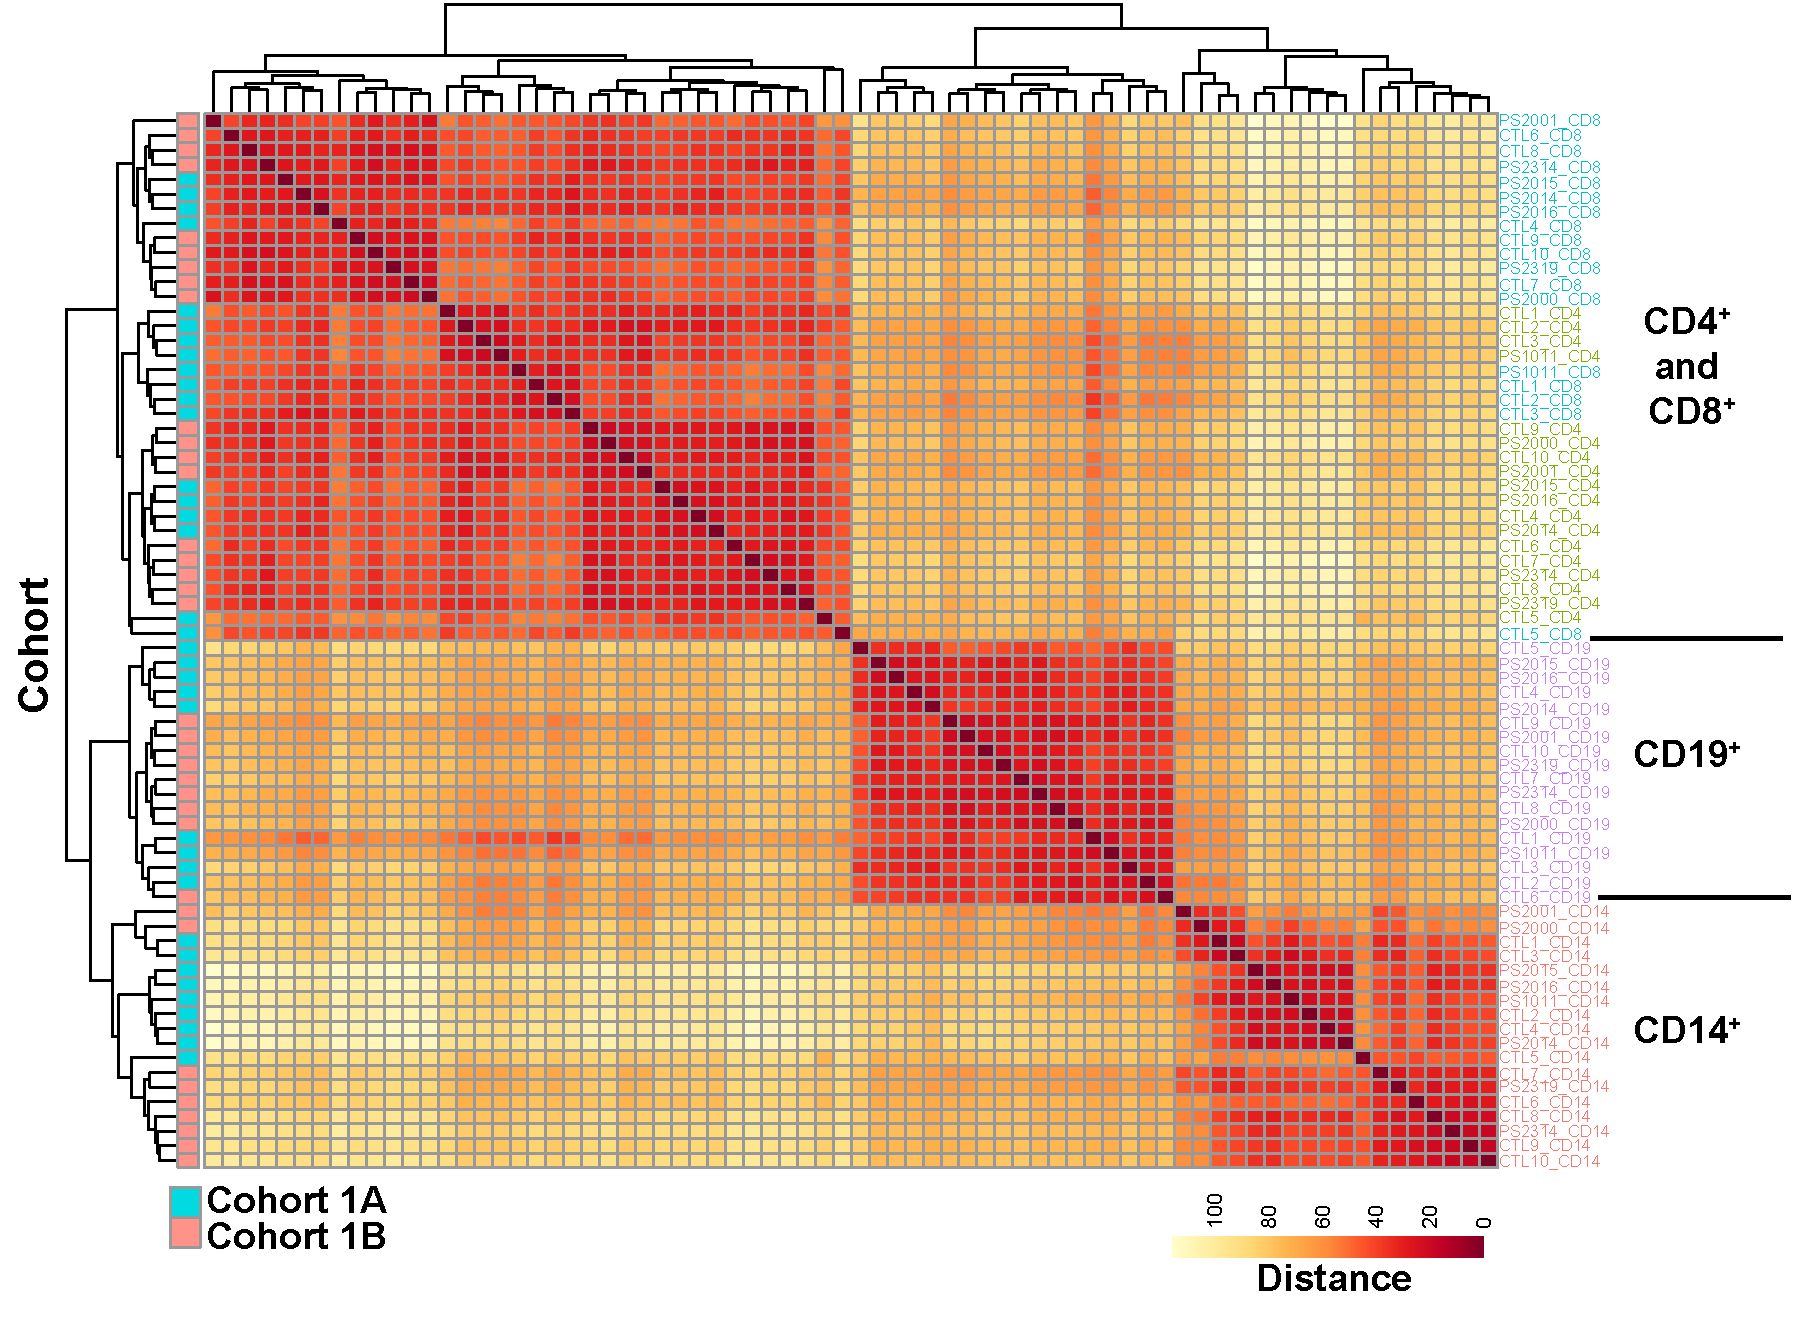
\includegraphics[width=\textwidth]{./Results2/pdfs/ATAC_all_cell_types_heatmap_with_batch_annotation}
\caption{}
\end{subfigure}
~
\begin{subfigure}[b]{0.6\textwidth} 
%the [b] prevents offset in subcaptions
\centering
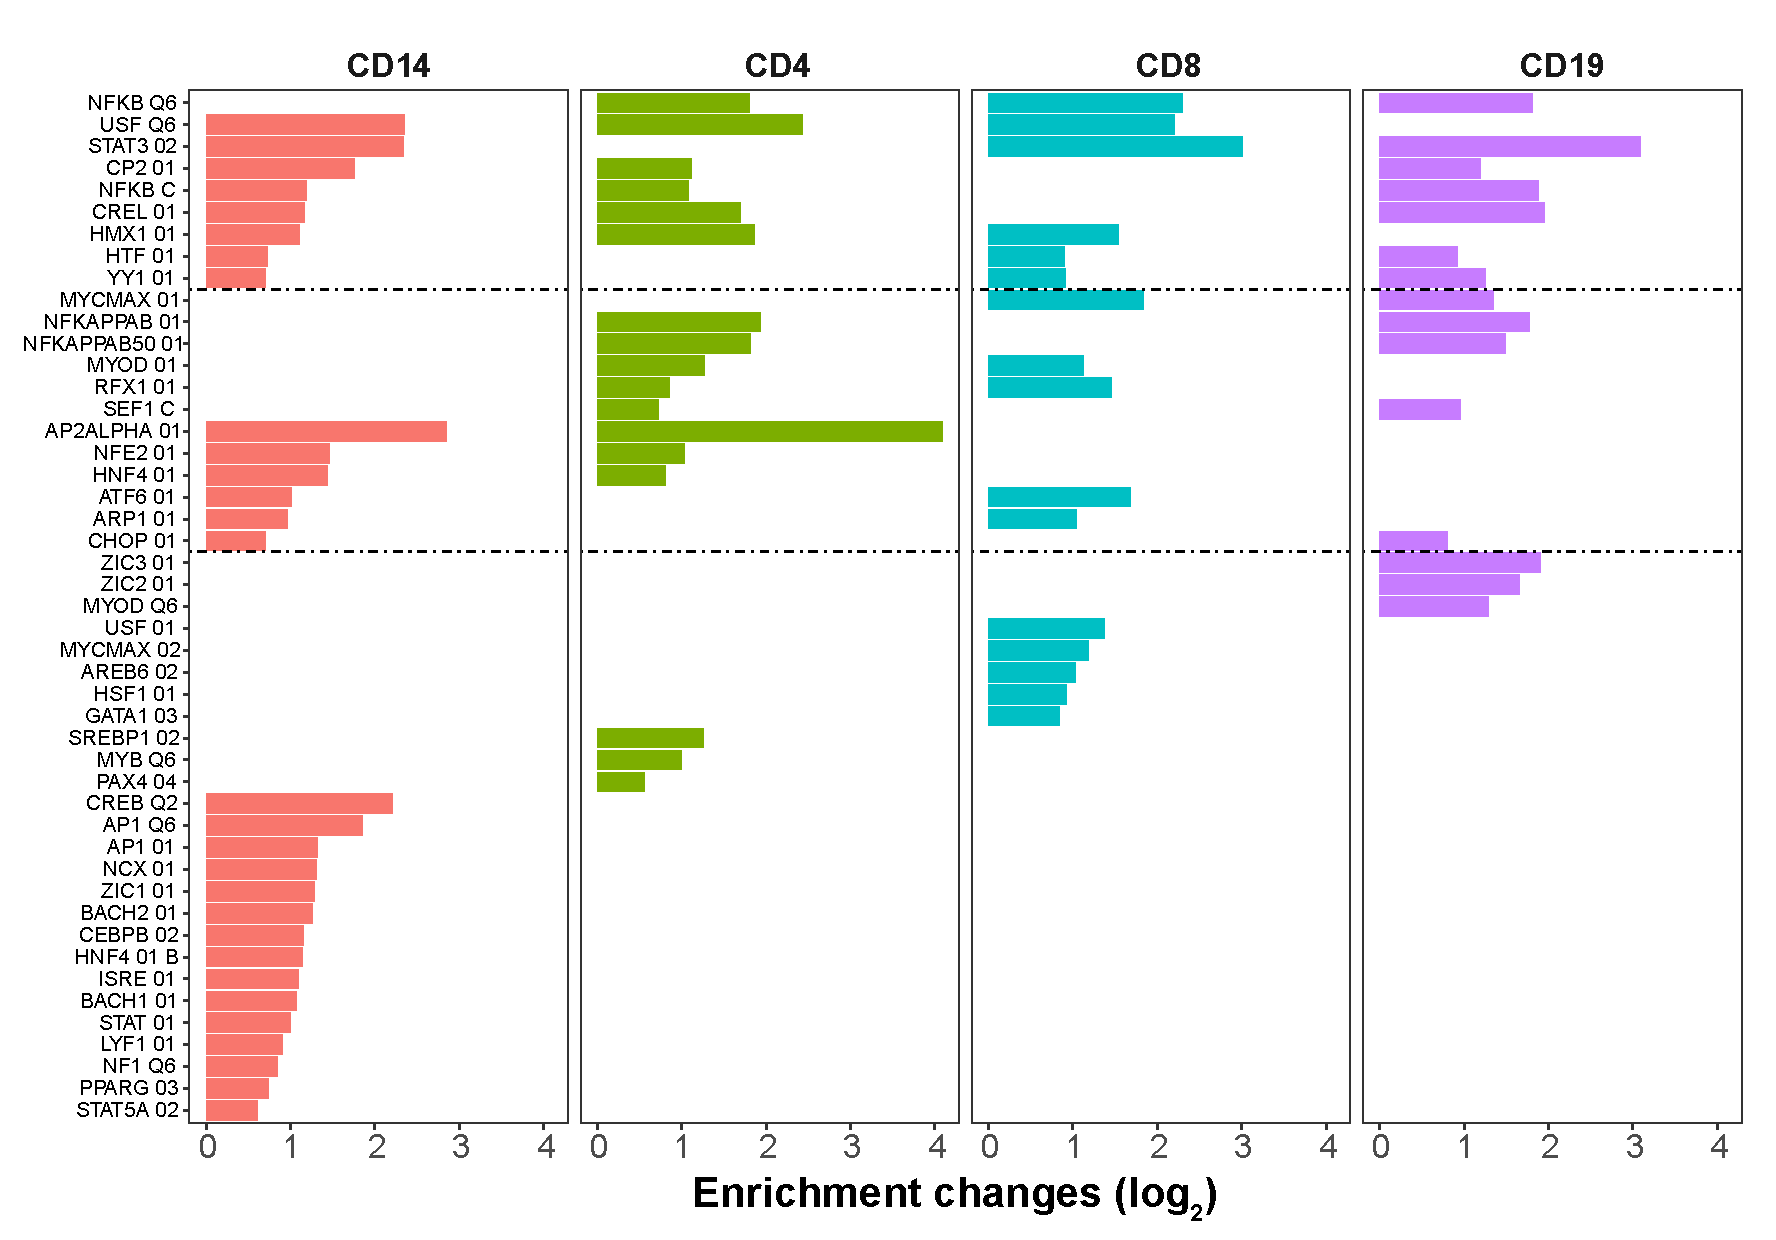
\includegraphics[width=\textwidth]{./Results2/pdfs/ATAC_PS_CTL_cell_type_specific_master_list_conserved_TFBS_enrichment}
\caption{}
\end{subfigure}
\caption[K-means clustered heatmap and conserved TFBS enrichment analysis in the consensus ATAC-seq regions identified in CD14$^+$ monocytes, CD4$^+$, CD8$^+$ and CD19$^+$ cells from the patients and controls cohort.]{\textbf{K-means clustered heatmap and conserved TFBS enrichment analysis in the consensus ATAC-seq regions identified in CD14$^+$ monocytes, CD4$^+$, CD8$^+$ and CD19$^+$ cells from the patients and controls cohort.} a) Distance matrix and k-means clustering for the 72 samples was performed based on the normalised read counts retrieved for each sample at the regions included in a consensus master list of ATAC-seq enriched sites built across all four cell types (MASTER\_ALL). Clusters have been additionally annotated using cohort identity. b) Enrichment analysis for the conserved TFBS was performed for each of the ATAC-seq cell type master lists of regions used for downstream differential analysis. Enrichment was tested for 258 human conserved TFBS identified by Transfac using a position-weight matrices based on experimental results in the scientific literature. Significant enrichment using FDR$<$0.01.}
\label{figure:ATAC_PS_CTL_heatmap_TFBS}
\end{figure}



Each of the four cell type master list of ATAC-seq peaks (ML\_CD14, ML\_CD4,ML\_CD8, and ML\_CD19), used for the downstream differential chromatin accessibility analysis (explained in Chapter \ref{ch:Mat}), presented the highest percentage of regions annotated as gene promoters, intronic and intergenic, as expected for ATAC-seq (Figure \ref{figure:ATAC_PS_CTL_genomic_annotation}). \textit{cis}-eQTL SNPs from a number of immune cell types, including CD14$^+$ monocytes (unstimulated and stimulated), B cells, neutrophils, CD4$^+$ and CD8$^+$ cells \parencite{Fairfax2012, Fairfax2014, Kasela2016}, were enriched within the ATAC-seq consensus peak list of each cell type. For example, eQTLs from unstimulated and stimulated (LPS or IFN-$\gamma$) monocytes presented greatest significant enrichment (FDR$<$0.01) in the ML\_CD14 (unstimulated fold-enrichment 5.1, LPS 2h fold-enrichment 4.7 and IFN-$\gamma$ fold-enrichment 5.0) when compared to the other eQTL datasets. Similarly, the \textit{cis}-eQTLs from the CD4$^+$ and CD8$^+$ were the most enriched datasets (fold-change 8.3 and 8, respectively) in the ML\_CD8. The relevance of each cell type master list was further reinforced by the significant enrichment (FDR$<$0.01) of conserved TFBS within those ATAC-seq regions (Figure \ref{figure:ATAC_PS_CTL_heatmap_TFBS} b). For example, enrichment of conserved NF$\kappa$B binding motifs(NFKB Q6, NFKB C and NFKAPPAB 01) was identified across the master lists from the different cell types. Similarly, conserved binding motifs fro TF involved in T cell biology , such as AREB6 (ZEB1), ATF6 and the heat-shock transcription factor HSF1 \parencite{Guan2018,Yamazaki2009,Gandhapudi2013}. 
%For example, enrichment of conserved binding motifs for AREB6 (ZEB1) involved in CD8$^+$ T effector and memory cell fate \parencite{Guan2018}, ATF6 implicated in NF$\kappa$B activation \parencite{Yamazaki2009} and the heat-shock transcription factor HSF1 regulator of T cell division under different types of stress \parencite{Gandhapudi2013} was found in the ML-CD8. 
Overall, the enrichment of eQTL SNPs and conserved TFBS highlighted the potential of each cell type master list to harbour functional relevant differences in chromatin accessibility between psoriasis patients and controls.

Differential chromatin accessibility analysis between patients and controls was performed on the ATAC-seq normalised read counts for the regions of each cell type master lists using DESeq2. PCA analysis on the normalised counts of each cell type master list prior to the differential analysis revealed a batch effect correlating with the different ATAC-seq protocols used in cohort 1A and cohort 1B (standard ATAC-seq and FAST-ATAC, respectively) (Figure \ref{figure:ATAC_RNAseq_batch_effect} a). Therefore, the ATAC-seq protocol was included as a covariate in the differential analysis model. Moreover, CTL5 appeared as a cohort 1A outlier for all the cell types (representative example Figure \ref{figure:ATAC_RNAseq_batch_effect} a) and was also removed from the differential analysis.

Genome-wide differential chromatin accessibility analysis revealed 55 significant (FDR$<$0.05) DARs between psoriasis patients and healthy controls in CD8$^+$ cells (Table \ref{tab:ATAC_PS_CTL_differential_analysis_results}). Conversely, CD14$^+$ monocytes, CD4$^+$ and CD19$^+$ cells only presented one or none DARs. 

% RANKL in RA  https://onlinelibrary.wiley.com/doi/full/10.1002/art.21731
% RANKL PsA https://www.ncbi.nlm.nih.gov/pmc/articles/PMC153764/

\begin{table}[htbp]
%\setlength{\tabcolsep}{20pt} only to stretch the columns if you want
%\renewcommand{\arraystretch}{1.5}
\centering
\begin{tabular}{@{} c c}
\toprule
\textbf{Cell type}   & \textbf{Number of DARs} \\
                     & \textbf{FDR$<$0.05}     \\
\midrule
\midrule
CD14$^+$             & 1 \\                 
CD4$^+$              & 0 \\
CD8$^+$              & 55 \\
CD19$^+$             & 1 \\
\bottomrule 
\end{tabular}
\medskip %gap
\caption[Summary results from the differential chromatin accessibility analysis between psoriasis patients and healthy controls in CD14$^+$ monocytes, CD4$^+$, CD8$^+$ and CD19$^+$ cells.]{\textbf{Summary results from the differential chromatin accessibility analysis between psoriasis patients and healthy controls in CD14$^+$ monocytes, CD4$^+$, CD8$^+$ and CD19$^+$ cells.} The number of differentially accessiblee regions (DARs) refers to those statistically significant when using a cut-off for background reads of 80\% (see Chapter \ref{ch:Results1} and an FDR$<$0.05. No threshold for the FC was applied in this analysis.}
\label{tab:ATAC_PS_CTL_differential_analysis_results}
\end{table}
\bigskip %bigger space


Annotation of the 55 CD8$^+$ DARs using cell type specific Roadmap Epigenomics chromatin segmentation map revealed the potential of some of those regions to be involve in regulation of gene expression, including 24 (44.4\%) weak enhancers, 7 (12.9\%) active promoters, 6 (11.1\%) weak promoter and 2 (3.7\%) strong enhancers. The functional relevance of the DARs in terms of regulation of gene expression was further investigated by integration of the CD8$^+$ cells eRNA data from the FANTOM5 project. Interestingly, only 8 of the CD8$^+$ DARs overlapped significantly expressed eRNAs. Amongst others, the DARs overlapping eRNA include a region at the TSS of the \textit{TNSF11} gene and another at a distal promoter from \textit{IL7R}, which were more accessible in the psoriasis patients compared to the healthy controls (Figure \ref{figure:ATAC_PS_CTL_CD8_TNFSF11_IL7R_tracks} a and b). The two DARs were also overlapping chromatin harbouring H3K4me3, a histone mark indicating an active promoter, and H3K27ac, mostly found at active enhancers, consistently with the overlap of those regions with FANTOM5 eRNAs in CD8$^+$.

\begin{figure}[htbp]
\centering
\begin{subfigure}{0.5\textwidth}
\centering
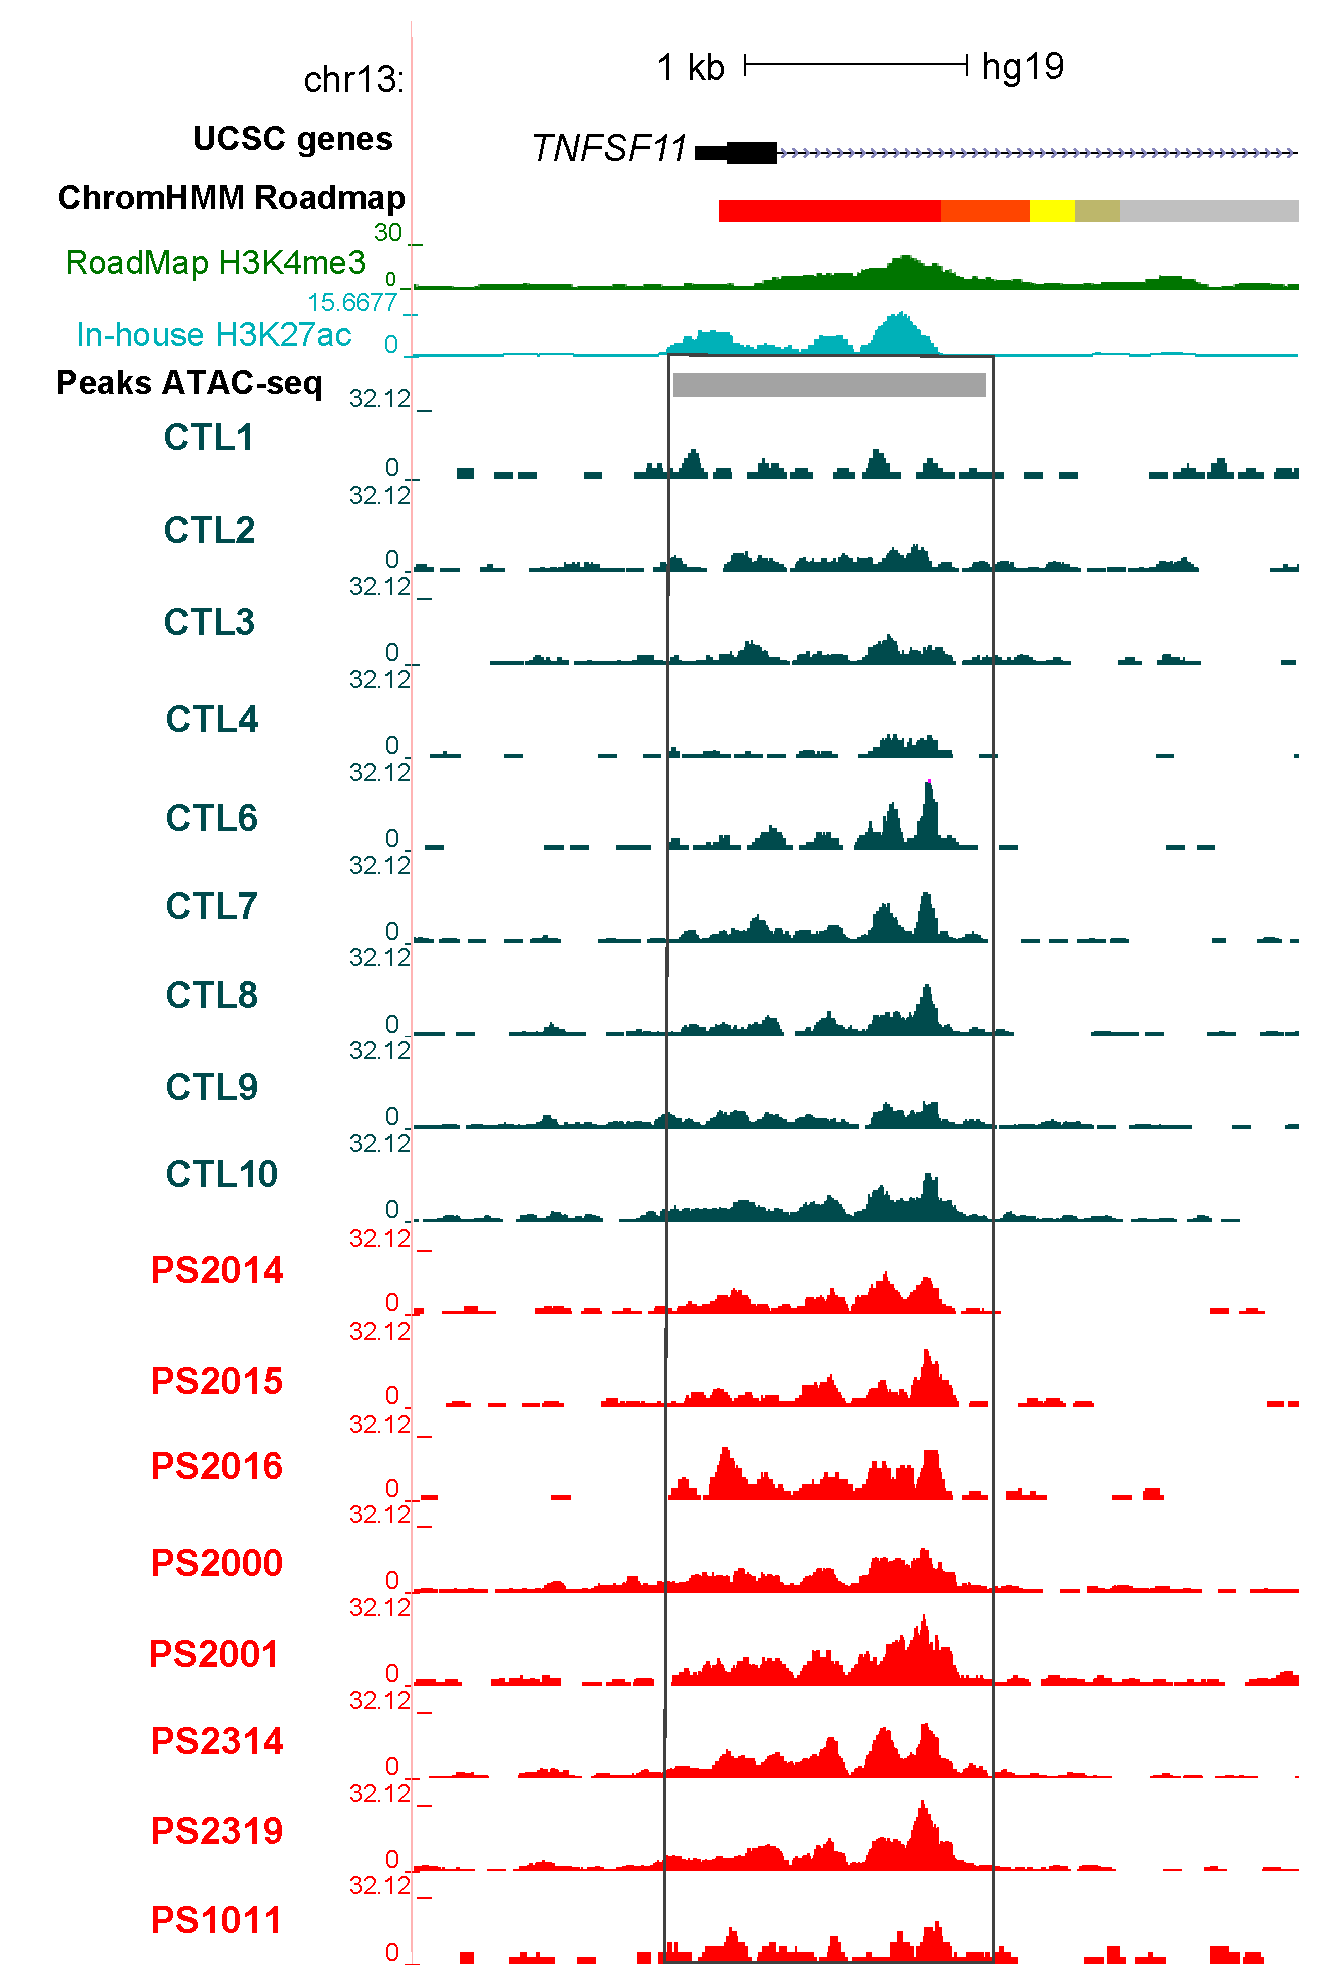
\includegraphics[width=\textwidth]{./Results2/pdfs/UCSC_ATAC_CD8_peak_prom_TNFSF11}
\caption{\textbf{}}
% The percentage sign indicated that the other subfig goes side by side
\end{subfigure}%
\begin{subfigure}{0.5\textwidth}
\centering
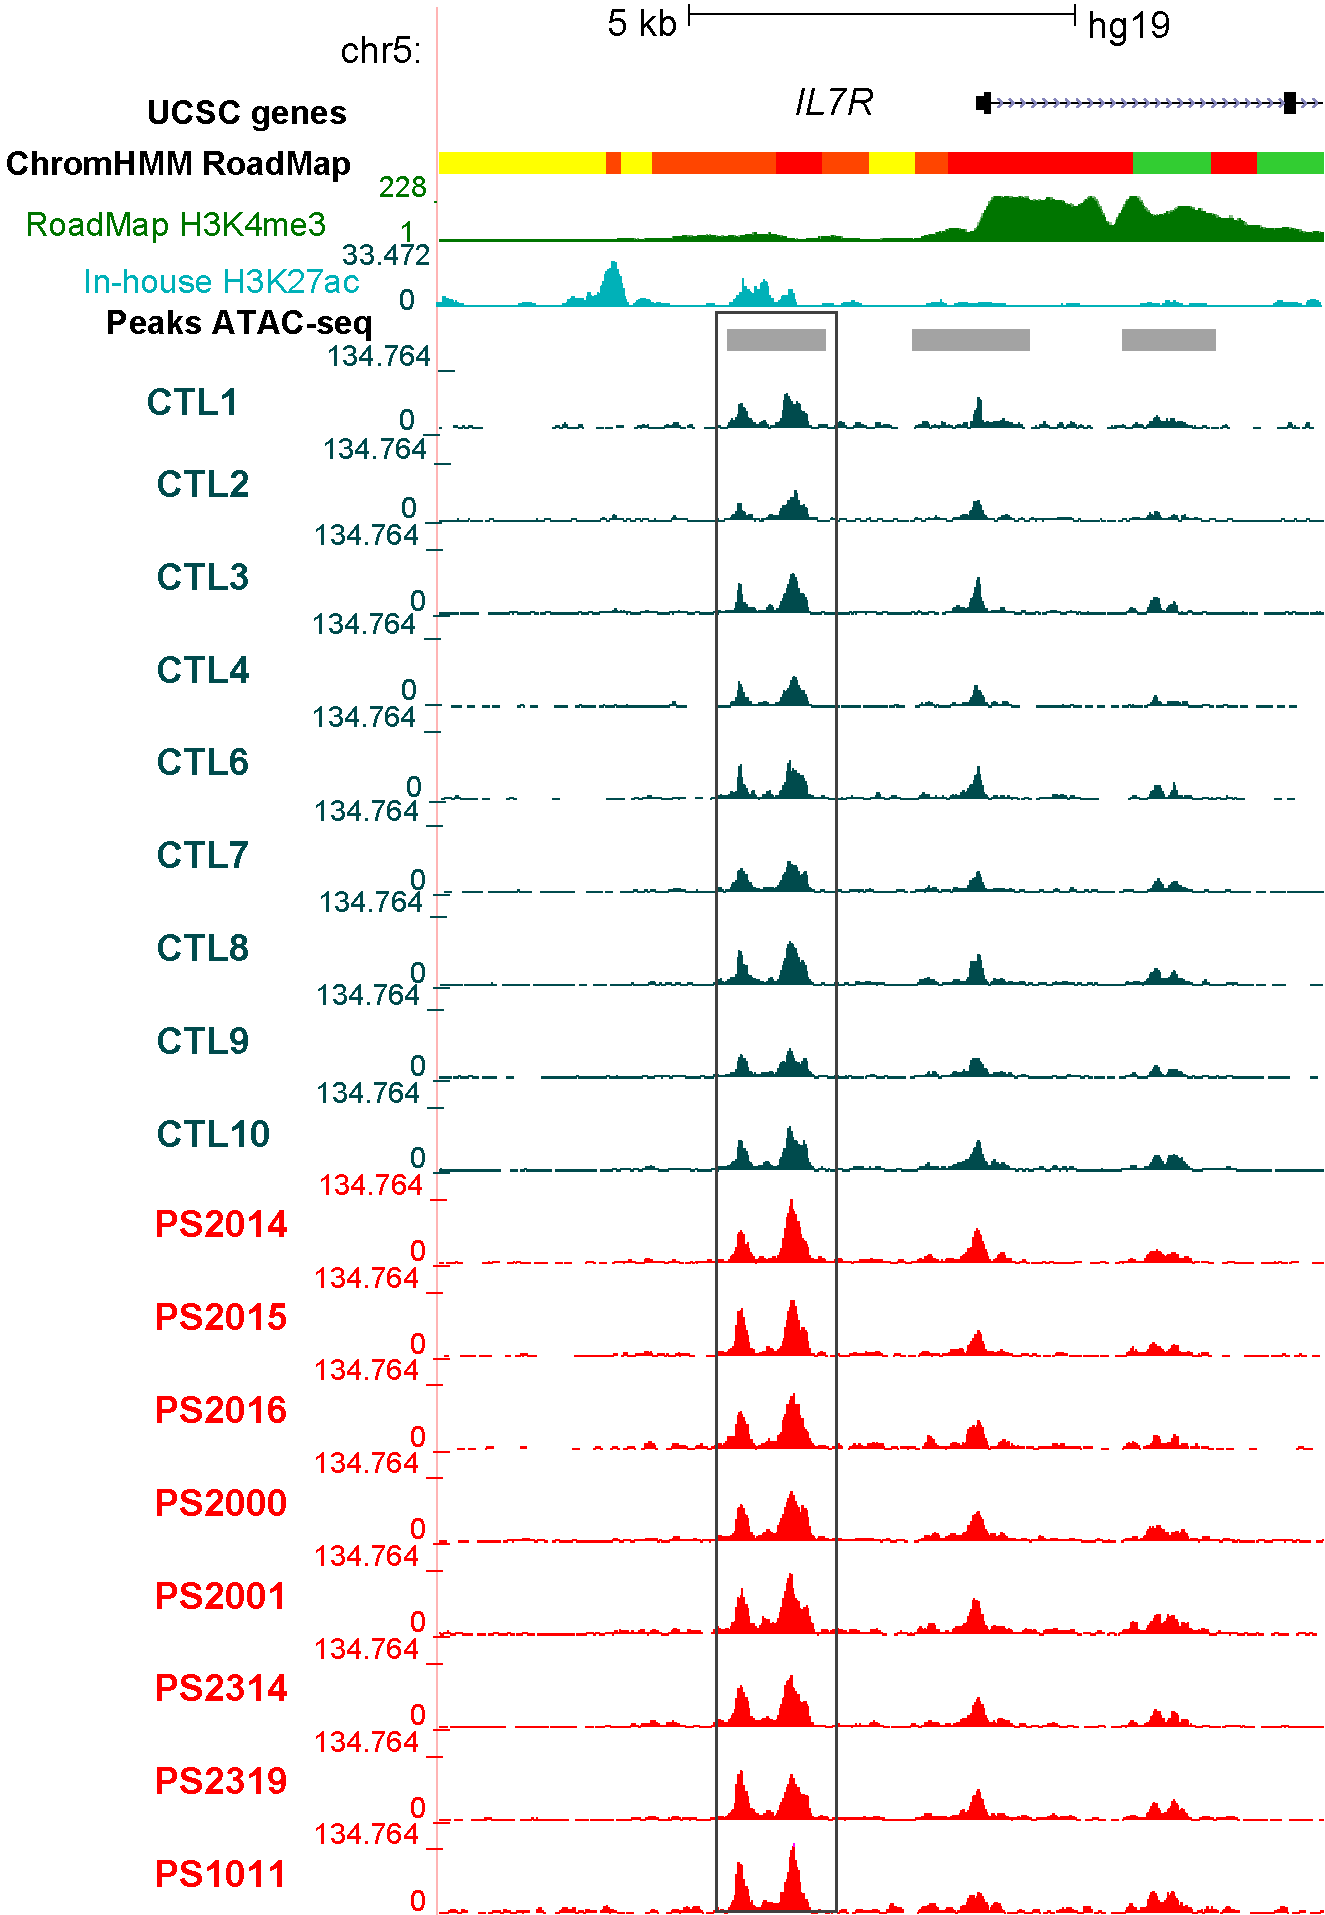
\includegraphics[width=\textwidth]{./Results2/pdfs/UCSC_ATAC_CD8_normalised_peak_enh_IL7R}
\caption{\textbf{}}
\end{subfigure}
\caption[Epigenetic landscape at two ATAC-seq differential accessible regions between patients and controls in CD8$^+$ cells.]{\textbf{Epigenetic landscape at two ATAC-seq differential accessible regions between patients and controls in CD8$^+$ cells.}xxx}
\label{figure:ATAC_PS_CTL_CD8_TNFSF11_IL7R_tracks}
\end{figure} 


Both of them are relevant genes in driving and maintaining the inflammatory response. For example, \textit{TNFSF11} is a cytokine from the TNF family involved in the regulation of T cell-dependent immune response and osteoclast differentiation in RA and PsA \parencite{Miranda‐Car\'ús2006,Ritchlin2003}. \textit{TNFSF11} is also downstream the lead SNPs for a CD risk locus \parencite{ImmunoBase}. Interestingly, the \textit{TNFSF11} protein, RANKL was found to be overexpressed in epidermis from psoriasis patients compared to controls and cutaneous lupus erythematosus, highlighting the role of this gene in the pathophysiology of psoriasis \parencite{Toberer2011}. On the other hand \textit{IL7R} is a proximal gene to SLE and MS, amongst others, and the axis IL-7/IL-7R has been found to drive IL7 indepdendent TNF-$\alpha$ inflammation in RA patients presenting iTNF resistence \parencite{van Roon2017}. Other potentially interesting CD8$^+$ DARs were found nearby genes such as the MAPK \textit{MAP3K7CL} and \textit{NFKB1}; However they were not at regions annotated as enhancers or overlaped with experimentally validated eRNAs. Additionally, none of the CD8$^+$ DARs were found within an LD block (r$^2$$\geq$0.8) of the psoriasis risk GWAS loci.

\subsubsection{Integration of H3K27ac ChIPm and ATAC-seq chromatin accessibility profiles}

After defining the H3K27ac and chromatin accessibility profiles in four psoriasis circulating immune cell, the next step was to investigate the commonalities in the disease specific changes characterised by the two epigenetic functional approaches. The overlap between the H3K27ac ChIPm and ATAC-seq differential sites between patients and controls only showed one shared region in CD8$^+$ T cells within an intron of the D-tyrosyl-tRNA deacylase 1 (\textit{DTD1}) gene (Figure). This region presented lower levels of H3K27ac (4 patients versus 4 controls) and was less accessible (8 patients and 9 controls) in the psoriasis patients when compared to the healthy controls (Figure). This differential region was annotated as an active enhancer according to the CD8$^+$ ChormHMM segmentation map and did not presente 3D interaction with the promoter of any gene according to Hi-C and promoter Hi-C data in total CD8$^+$ cells \parencite{Javierre2016, }. Conversely, SNPs within this region appeared a significant eQTL for \textit{DTD1} expression in whole (https://gtexportal.org/home/eqtls). The role of this gene has been described in the initiation of DNA replication and has been associated with aspirine-intolerance in asthmatics \parencite{Pasaje2011}. However, no studies have yet highlighted a direct link of this gene with the pathophysiology of chronic inflammatory diseases.  

Altogether, these results suggest that differences in H3K27ac are not driving the genome-wide changes in chromatin accessibility between psoriasis patients and healthy controls in total CD8$^+$ cells in this data. 

\begin{figure}[htbp]
\centering
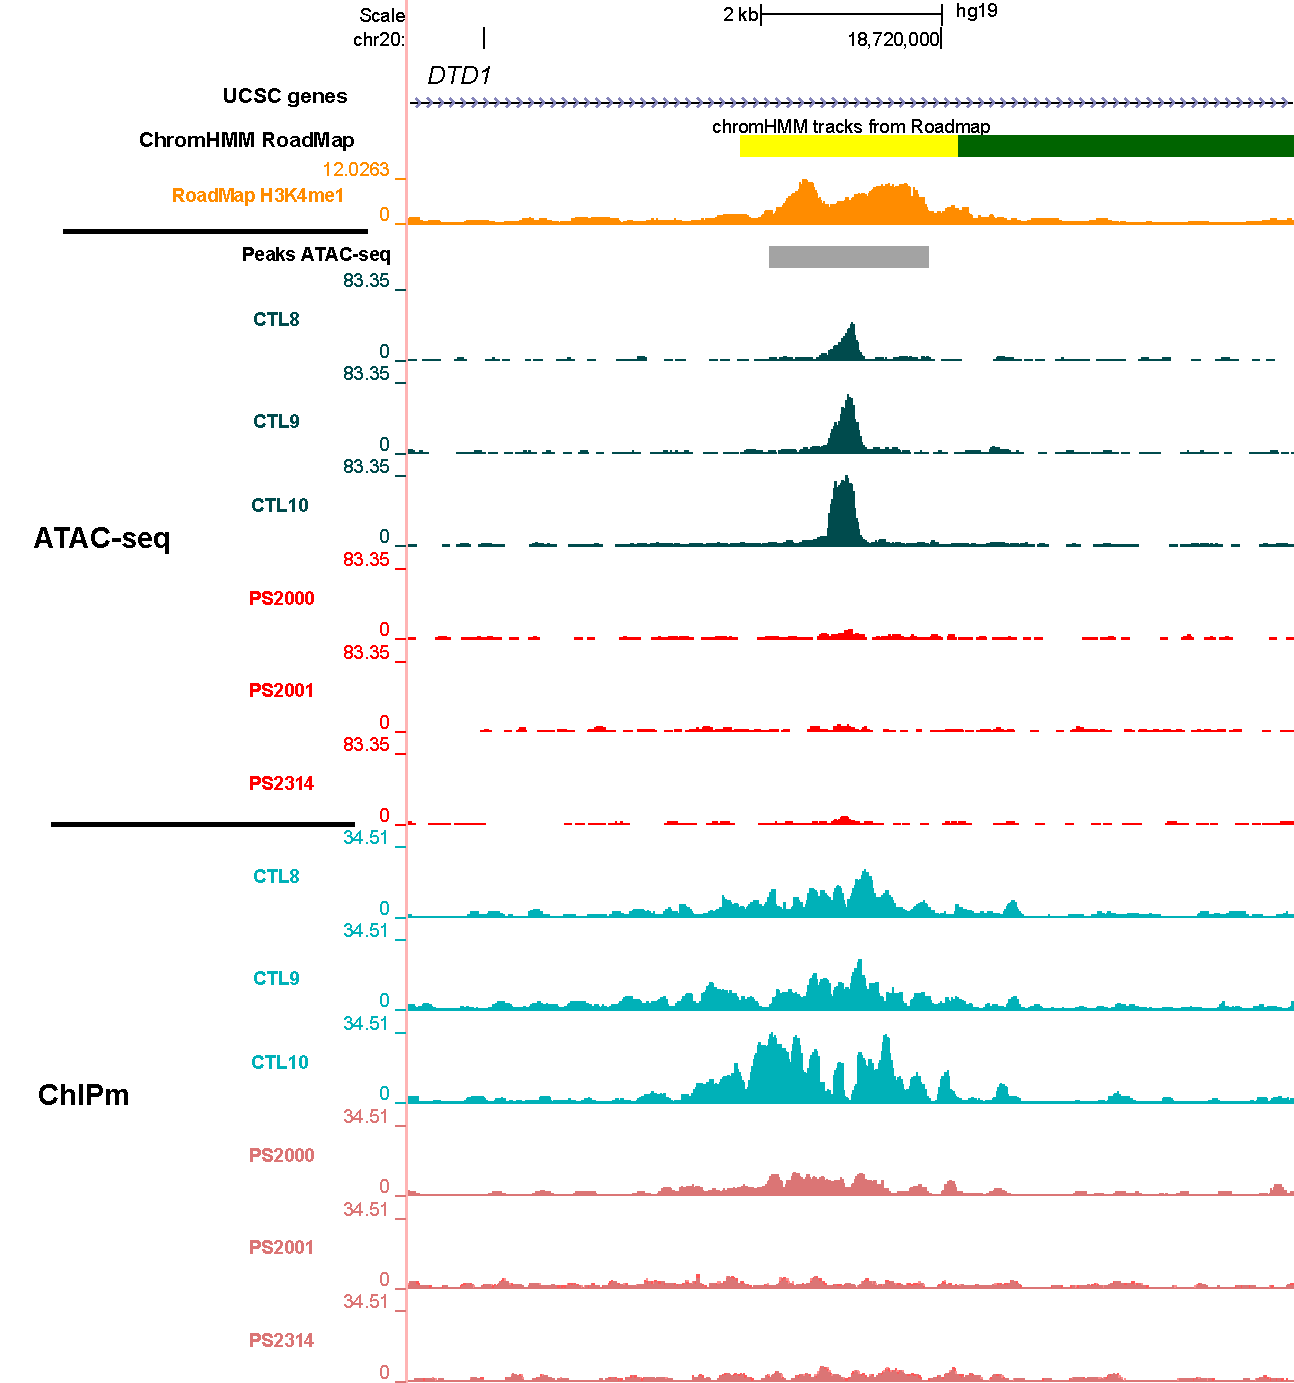
\includegraphics[width=0.6\textwidth]{./Results2/pdfs/ChIPm_H3K27ac_UCSC_CD8_DTD1_track}
\caption[Epigenetic landscape at the chr3:121,675,048-121,677,505 enhancer in circulating CD14$^+$ monocytes from psoriasis patients and healthy controls.]{\textbf{Epigenetic accessibility landscape at the chr3:121,675,048-121,677,505 enhancer in circulating CD14$^+$ monocytes from psoriasis patients and healthy controls.} Describe the track }
\label{figure:ChIPm_H3K27ac_UCSC_ILDR1_track}
\end{figure}


\subsection{Differential gene expression in psoriasis circulating immune cells}

\subsubsection{Assessing quality control of the RNA-seq data}
In addition to characterising the chromatin accessibility landscape, gene expression profiles in psoriasis and healthy individuals were also analysed for the same four primary circulating immune cell types using RNA-seq. The percentage of RNA-seq mapping to a unique location in the genome using STAR algorithm (see Chapter \ref{ch:Mat}) was appropriate (minimum recommended 70 to 80\%), ranging between 79.64 and 86.19\% ( CD8$^+$ CTL3 and CD14$^14$ monocytes CTL8, respectively) across all the 72 samples generated across the four cell types in psoriasis and control samples (Figure \ref{figure:RNAseq_mapping_rate_and_reads_in_genes} a). After appropriate filtering of non-uniquely mapped and duplicated reads, all the samples presented a minimum of 20 total million reads (as required by ENCODE standards) mapping to a comprehensive list of Ensembl features, including protein coding genes and lncRNAs (Figure \ref{figure:RNAseq_mapping_rate_and_reads_in_genes} b). The median of total million reads mapping to Ensembl features was greater for CD14$^+$ monocytes when compared to the other three cell types. However, the difference in medians across the four cell types did not exceed in more than 5 million reads. Interestingly, in all four cell types analysed, greater mapping rates and total million of reads mapping to Ensembl features were observed for cohort 1B samples when compared to cohort 1A. These differences were attributed to the library preparation and sequencing of each cohort in two different batches.  

\begin{figure}[htbp]
\centering
\begin{subfigure}{0.5\textwidth}
\centering
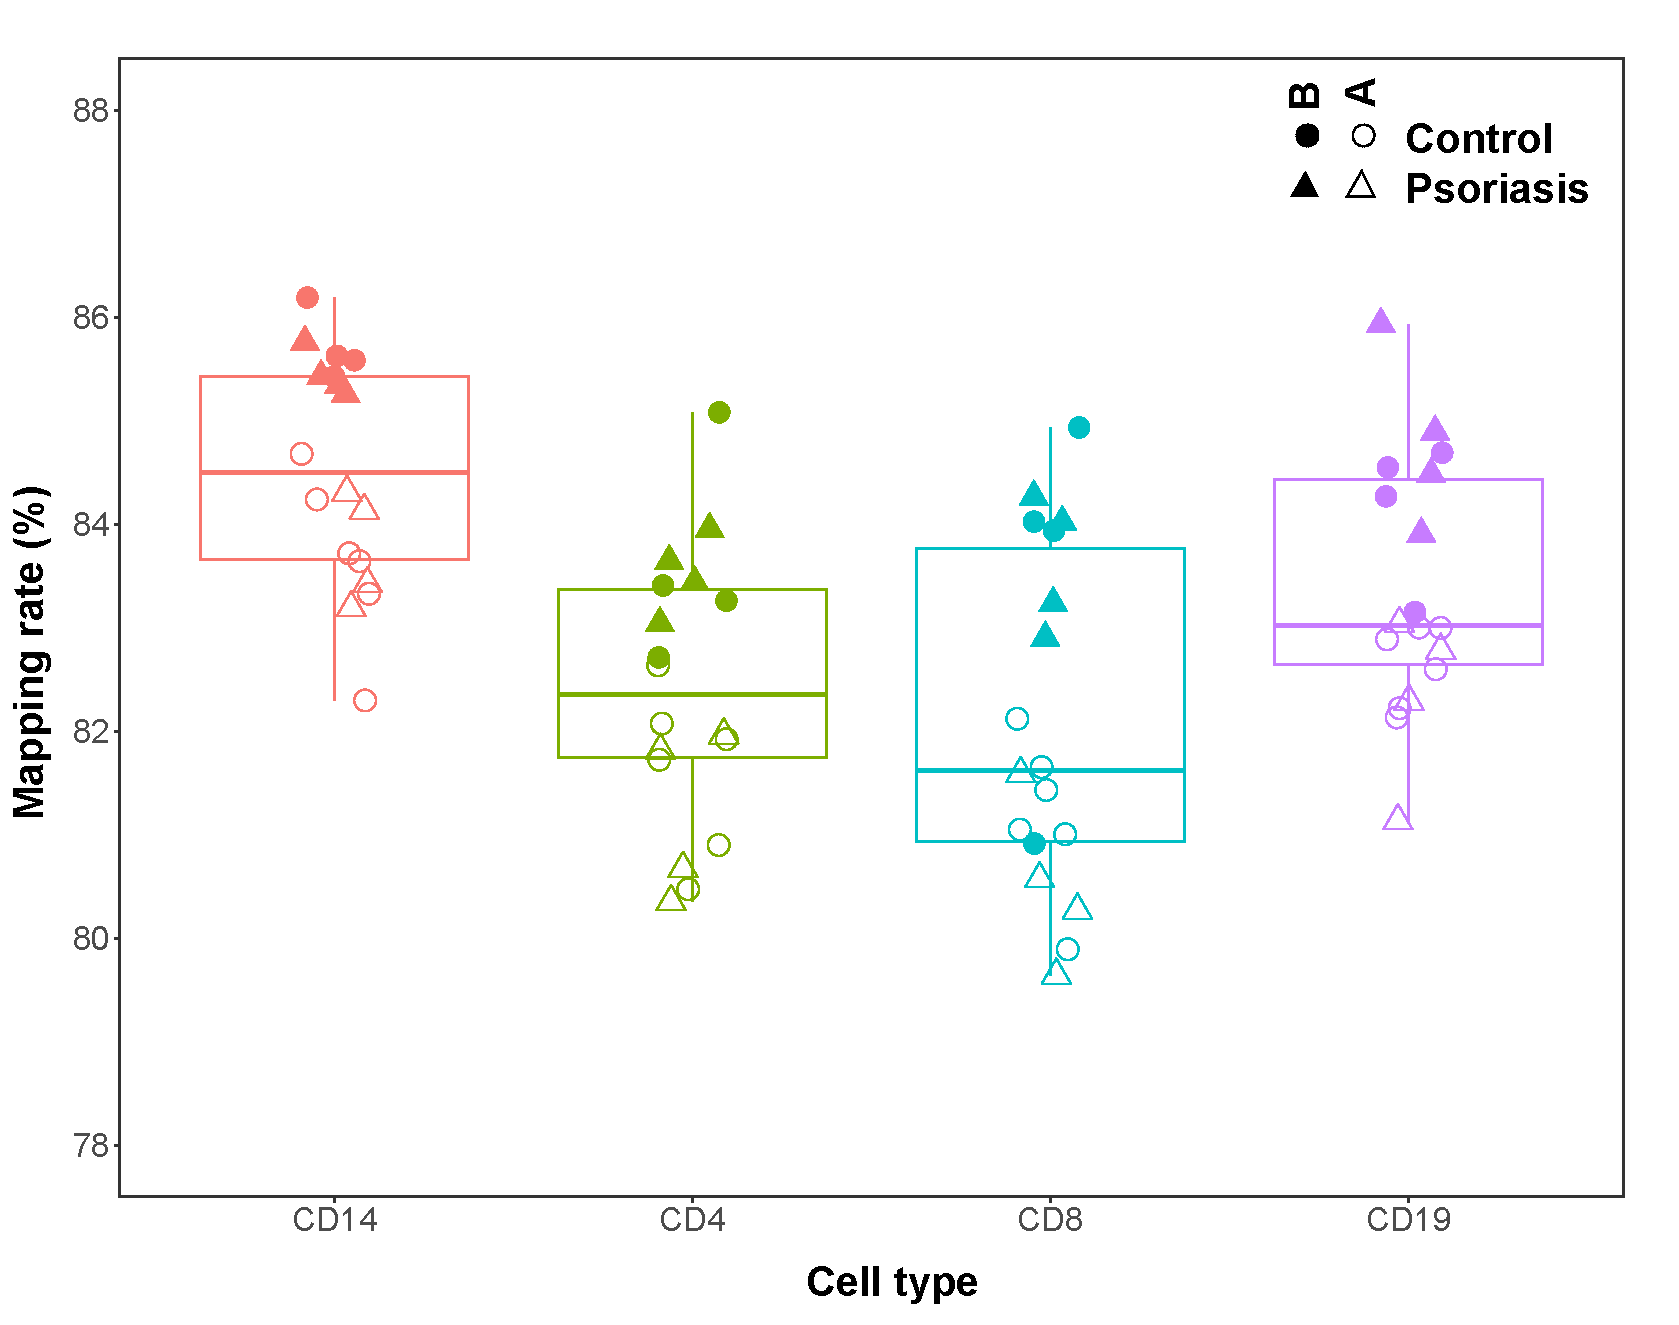
\includegraphics[width=\textwidth]{./Results2/pdfs/PS_CTL_RNAseq_uniquely_mapped_reads_rate_cell_type_batch_and_condition_boxplots}
\caption{\textbf{}}
% The percentage sign indicated that the other subfig goes side by side
\end{subfigure}%
\begin{subfigure}{0.5\textwidth}
\centering
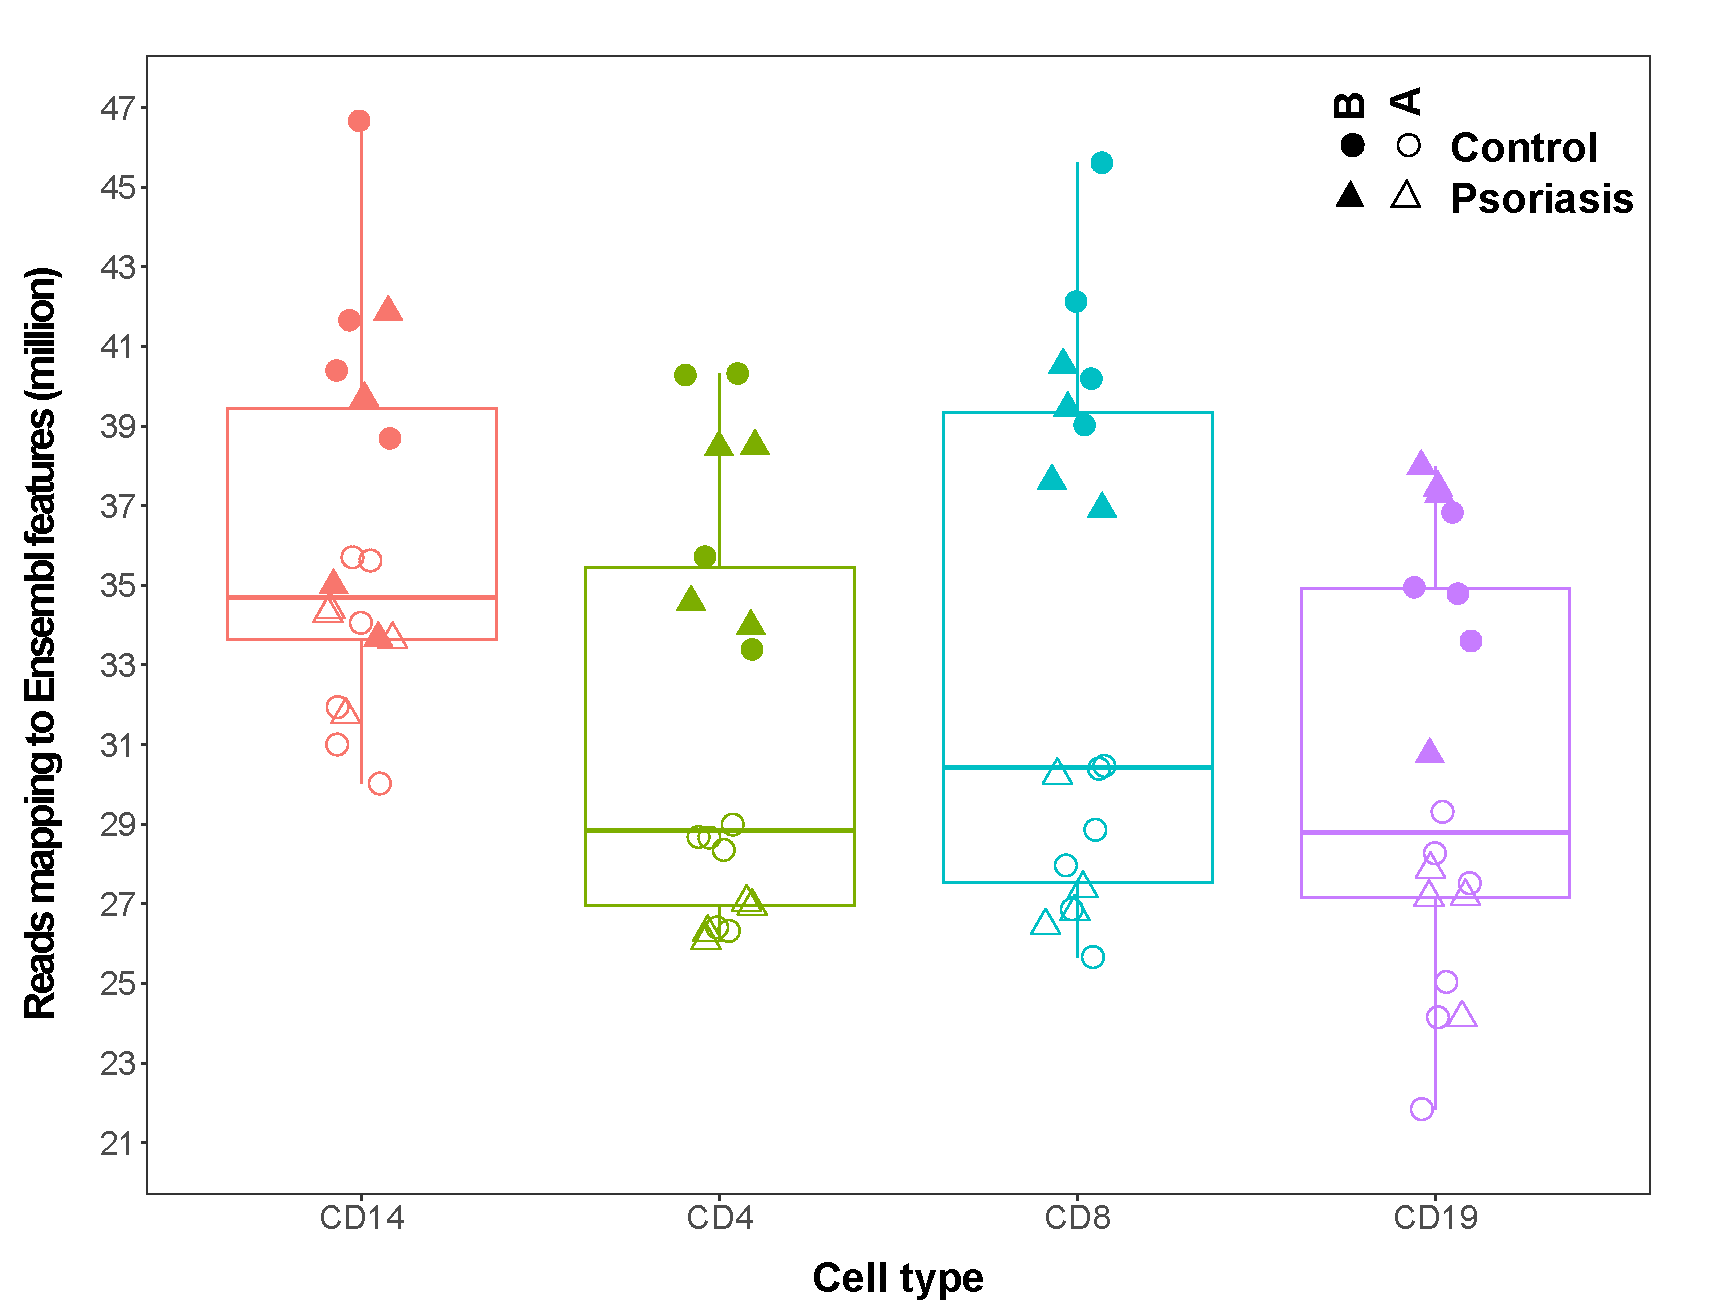
\includegraphics[width=\textwidth]{./Results2/pdfs/PS_CTL_RNAseq_total_reads_per_batch_cell_type_and_condition}
\caption{\textbf{}}
\end{subfigure}
\caption[Mapping rate and total reads after filtering (million) mapping to Ensembl genes in all the RNA-seq samples from psoriasis patients and controls in four cell types.]{\textbf{Mapping rate and total reads after filtering (million) mapping to Ensembl genes in all the RNA-seq samples from psoriasis patients and controls in four cell types.} a) The mapping rate refers to the percentage of total sequenced reads from each sample that uniquely mapped to a particular site of the genome. b) The total number of reads after filtering for non-uniquely mapped and duplicated reads that mapped to Ensembl features, including coding protein genes and lncRNAs.}
\label{figure:RNAseq_mapping_rate_and_reads_in_genes}
\end{figure} 


Similarly to ChIPm and ATAC-seq, the first and second PC from PCA analysis using the normalised number of reads mapping to each the 20,493 Ensembl genes passing quality control (see Chapter \ref{ch:Mat}) showed that most of variability was driven by cell type differences (Figure \ref{figure:RNAseq_PCA_and_heat_map} a). A heatmap illustrating sample distance based on the expression profile of each sample followed by k-means clustering revealed three main clusters corresponding to CD14$^+$ monocytes, CD4$^+$ and CD8$^+$ lymphocytes and CD19$^+$ cells (Figure \ref{figure:RNAseq_PCA_and_heat_map} a). Within each of cell type clusters, samples were further grouped by cohort (1A and 1B) and not by condition (psoriasis and control), consistently with the previous differences in mapping rate and total million reads mapping to Ensembl genes observed across the two cohorts (Figure \ref{figure:RNAseq_mapping_rate_and_reads_in_genes} a and b). This was reinforced by the clear correlation of sample batch with PC4 from the PCA analysis, which led to a very clear separation of the samples by cohort 1A and 1B, explaining 3\% of the total variance (Figure \ref{figure:ATAC_RNAseq_batch_effect} b). Consequently, cohort identity was included in the differential gene expression model as a covariate. 

\begin{figure}[htbp]
\centering
\begin{subfigure}{0.5\textwidth}
\centering
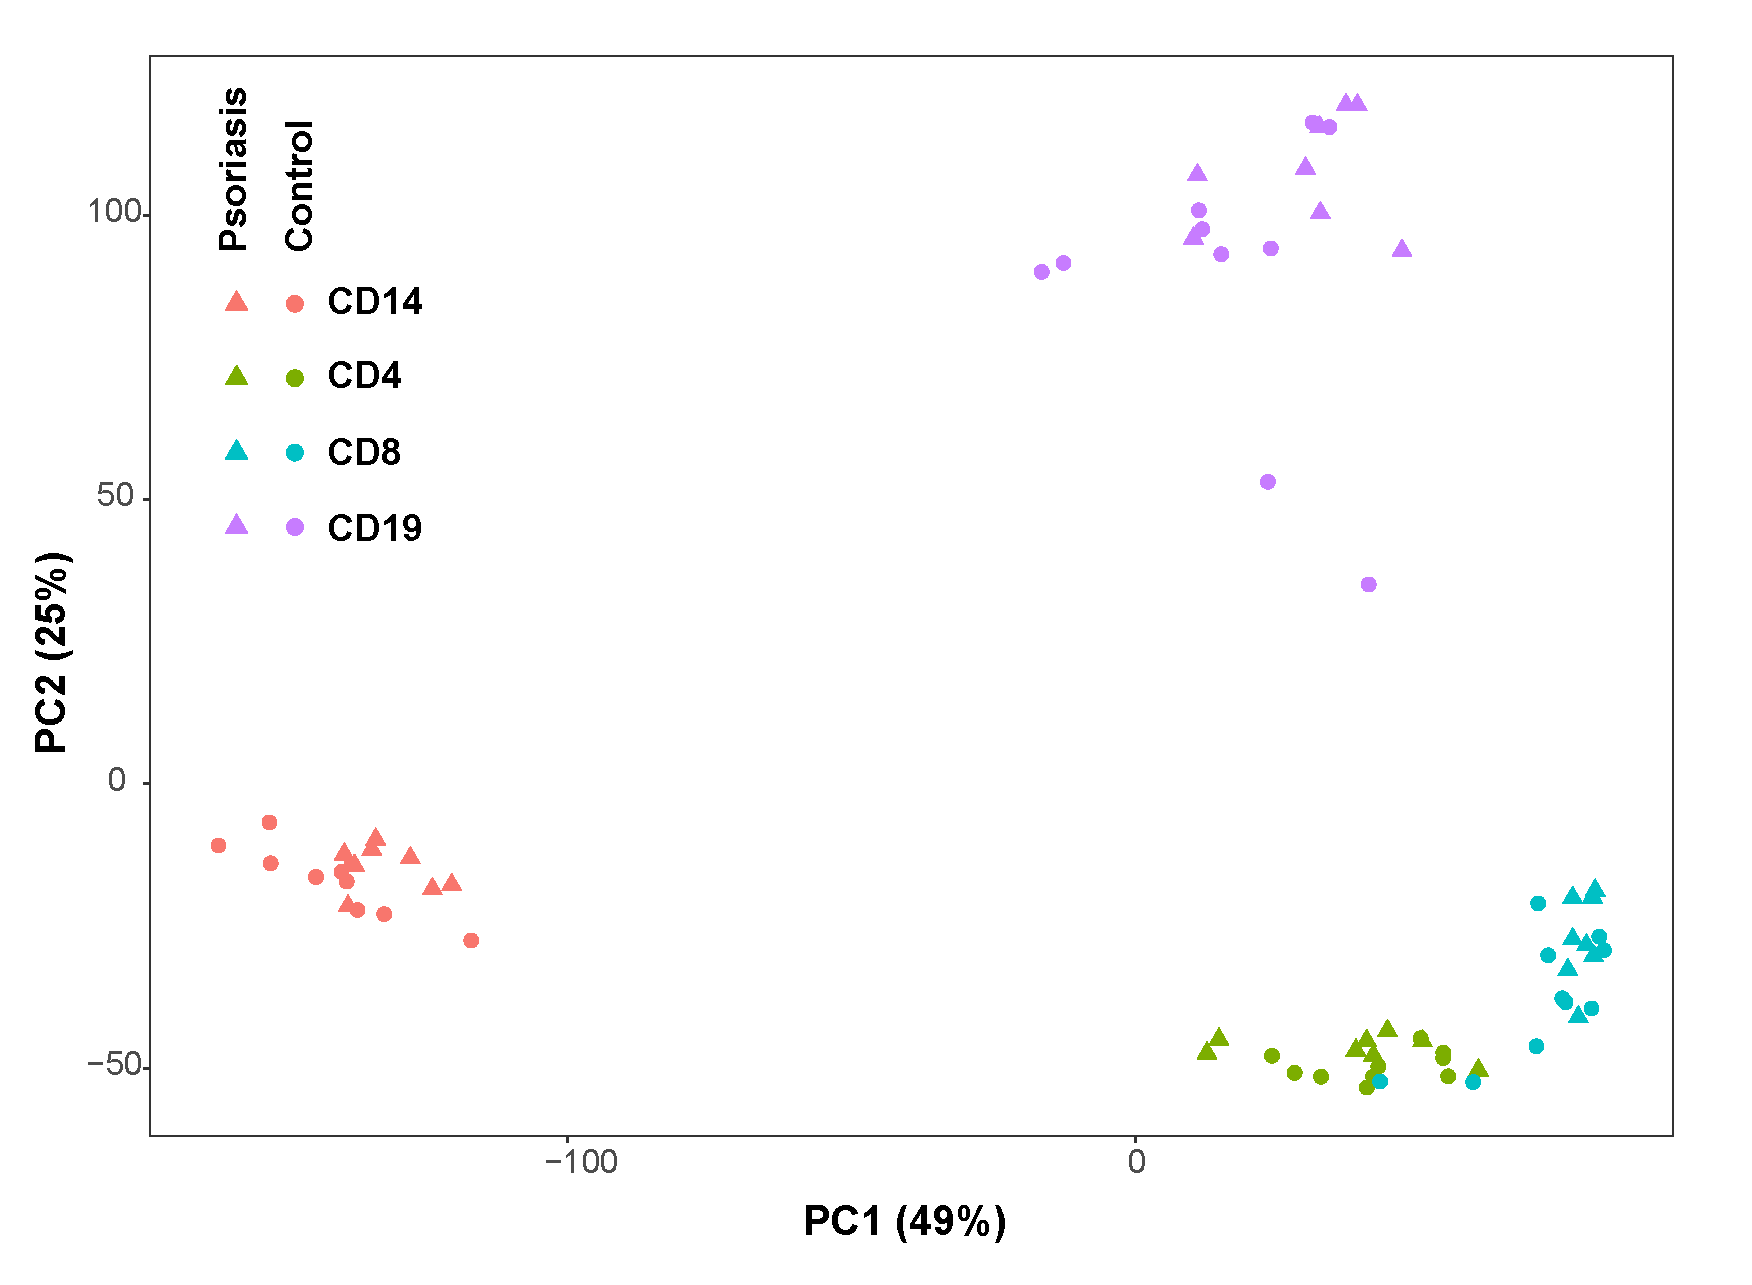
\includegraphics[width=\textwidth]{./Results2/pdfs/PS_CTL_all_samples_varied_PCA1and2_plot}
\caption{\textbf{}}
% The percentage sign indicated that the other subfig goes side by side
\end{subfigure}
\begin{subfigure}{0.5\textwidth}
\centering
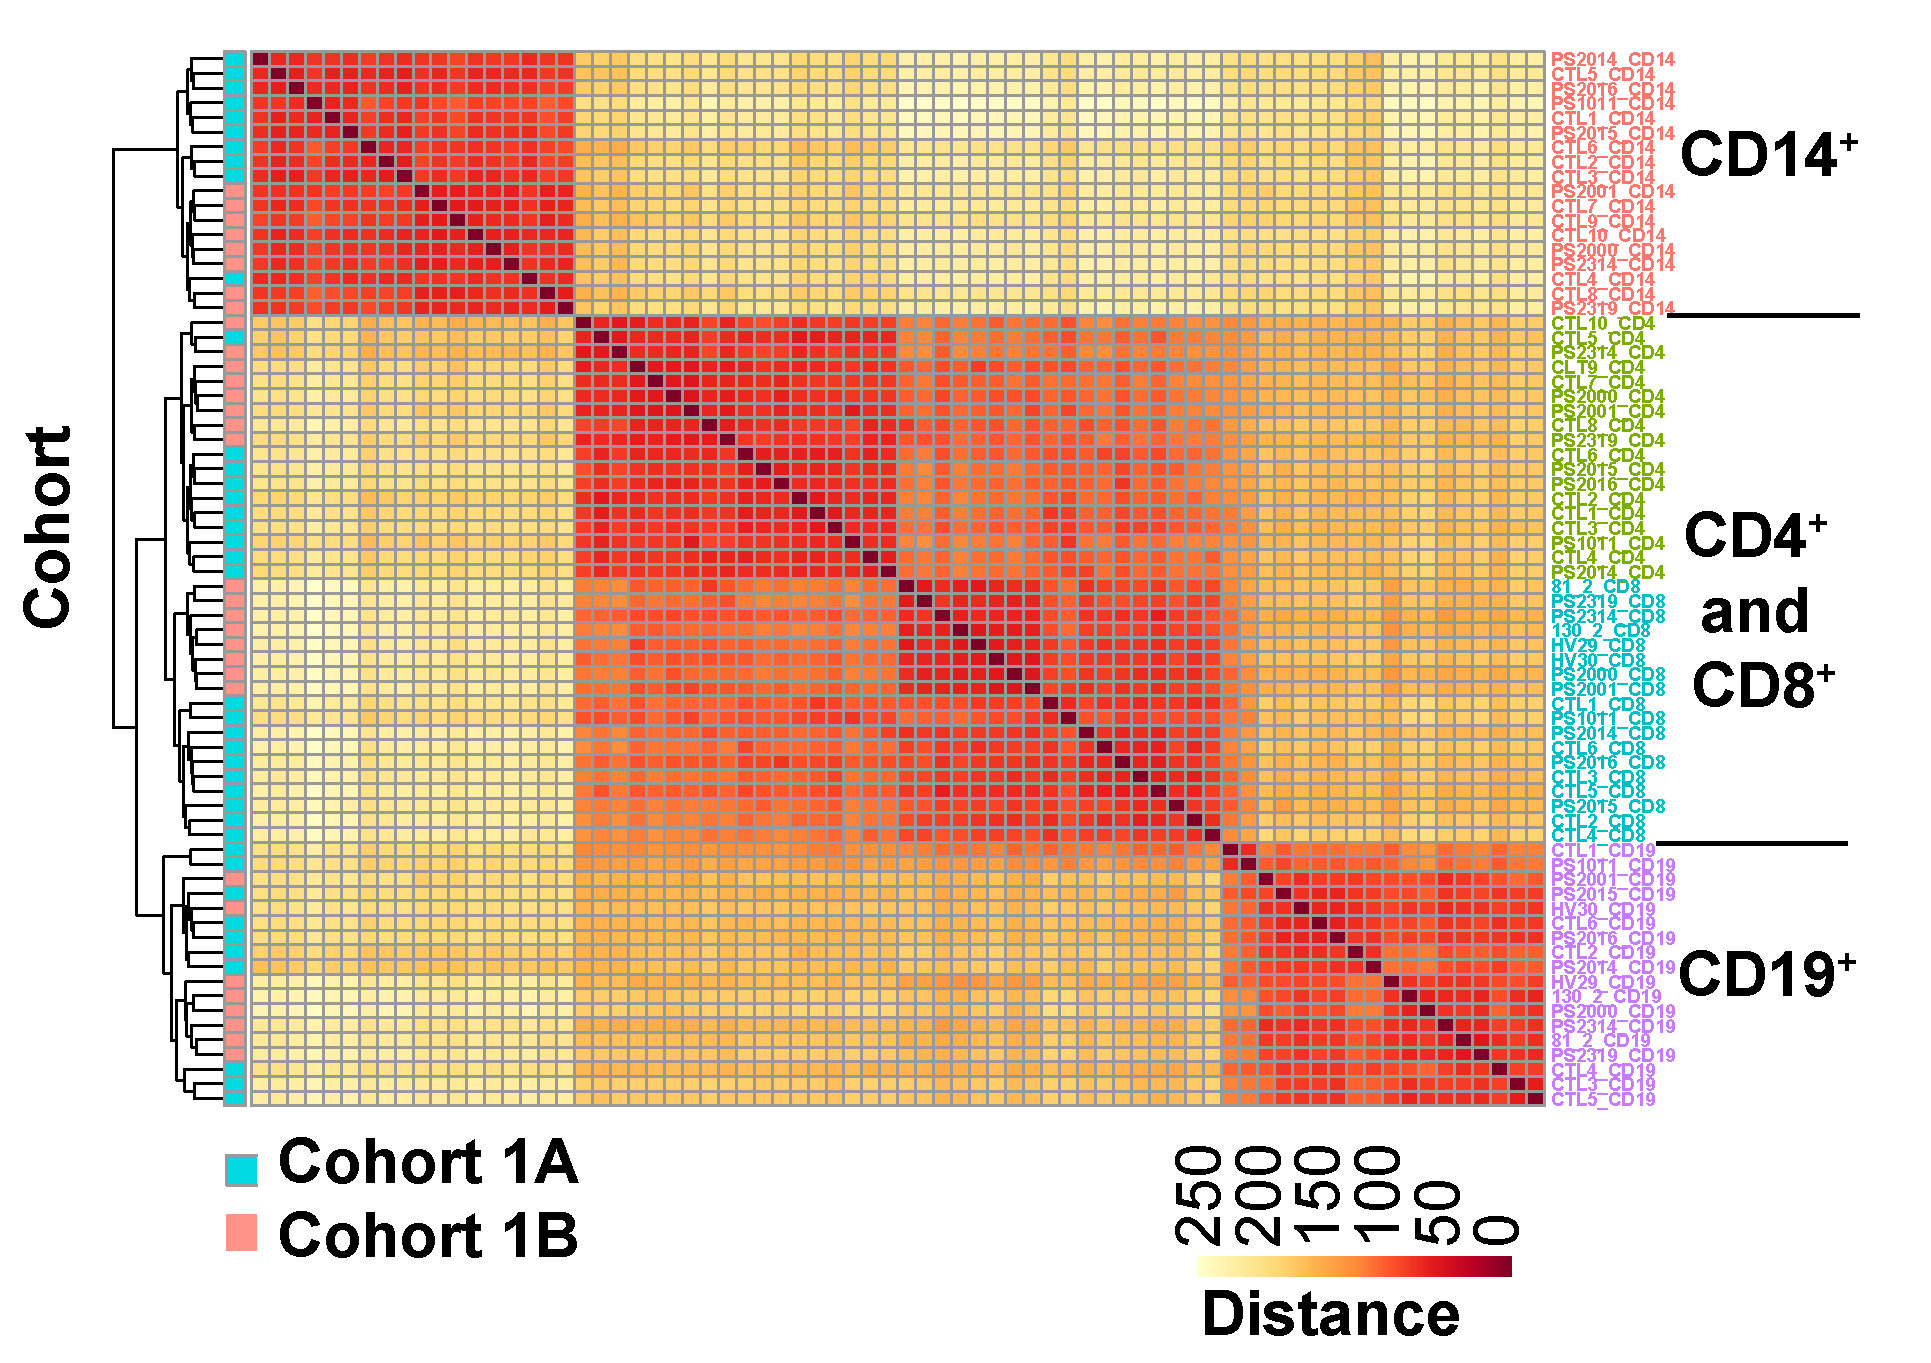
\includegraphics[width=\textwidth]{./Results2/pdfs/PS_CTL_all_samples_heatmap_including_batch}
\caption{\textbf{}}
\end{subfigure}
\caption[PCA analysis and  sample distance heatmap with k-means clustering illustrating the sample variability based on the gene expression profiles.]{\textbf{PCA analysis and  sample distance heatmap with k-means clustering illustrating the sample variability based on the gene expression profiles.} a) The first and second PCs (x-axis and y-axis, respectively) for the analysis using all the ML\_all regions are represented to identify the main sources of variability across the 72 samples. Each point represents a sample, where the colour codes for cell type and the shape for condition. The proportion of variation explained by each principal component is indicated.b) Distance matrix and k-means clustering for the 72 samples was performed based on the normalised read counts mapping to 20,493 Ensembl featured remaining after appropriate filtering. Annotation of the clustering using cohort identity is included.}
\label{figure:RNAseq_PCA_and_heat_map}
\end{figure}


\subsubsection{mRNA and lncRNA differential expression}

DGE between 8 psoriasis patients and 10 healthy controls in CD14$^+$ monocytes, CD4$^+$, CD8$^+$ and CD19$^+$ was performed using DESeq2 and including the cohort identity as a covariate to account for the batch effect previously mentioned. For each of the cell types a number of mRNAs were identified as differentially expressed for an FDR lower than 0.05 or 0.01 (Table \ref{tab:RNAseq_PS_CTL_differential_analysis_results}). 

\begin{table}[htbp]
%\setlength{\tabcolsep}{20pt} only to stretch the columns if you want
%\renewcommand{\arraystretch}{1.5}
\centering
\begin{tabular}{@{} c c c}
\toprule
\textbf{Cell type}   & \textbf{mRNA}            & \textbf{lncRNA}                \\
                     & \textbf{FDR$<$0.05/0.01} & \textbf{FDR$<$0.05/0.01}   \\
\midrule
\midrule
CD14$^+$             & 671/229 & 28/8\\                 
CD4$^+$              & 108/40  & 12/4\\
CD8$^+$              & 656/175 & 31/5\\
CD19$^+$             & 167/71  & 6/2\\
\bottomrule 
\end{tabular}
\medskip %gap
\caption[Summary results from the DGE analysis between psoriasis patients and healthy controls in CD14$^+$ monocytes, CD4$^+$, CD8$^+$ and CD19$^+$ cells.]{\textbf{Summary results from the DGE analysis between psoriasis patients and healthy controls in CD14$^+$ monocytes, CD4$^+$, CD8$^+$ and CD19$^+$ cells.} The number of statistically differentially expressed mRNAs and lncRNAs are listed for two FDR threshold (FDR$<$0.05 and FDR$<$0.01). No threshold for the FC was applied in this analysis.}
\label{tab:RNAseq_PS_CTL_differential_analysis_results}
\end{table}
\bigskip %bigger spac

CD14$^+$ monocytes and total CD8$^+$ were the two cell types presenting the largest number of mRNAs with modulated expression between psoriasis patients and controls. The more dysregulated gene expression response between patients and controls found in circulating psoriasis CD8$^+$ when compared to the CD4$^+$ may suggest the same hypothesis as in skin, where CD8$^+$ are considered the main effector cells undergoing activation upon the inflammatory stimuli \parencite(Nickoloff1999). Interestingly, CD19$^+$ presented greater number of differentially expressed mRNAs than CD4$^+$, regardless their up to date absence of implication in disease (confirm).

The magnitud in the FC of gene expression between psoriasis patients and controls was moderate in all four cell types, showing the largest changes in CD14$+$ monocytes and CD8$^+$ cells. Regarding the directionality of the statistically significant modulated genes (mRNa and lncRNAs) using FDR$<$0.05, CD14$^+$ monocytes (up 344, down 379) and CD4$^+$ (up 57, down 66) presented  similar number of genes up-regulated and down-regulated in psoriasis patients when compared to the healthy controls. In contrast, CD8$^+$ (up 278, down 429) CD19$^+$ (up 29, down 148) a largest number of modulated genes were down-regulated in patients compared to controls.



\begin{figure}[htbp]
\centering
\begin{subfigure}{0.5\textwidth}
\centering
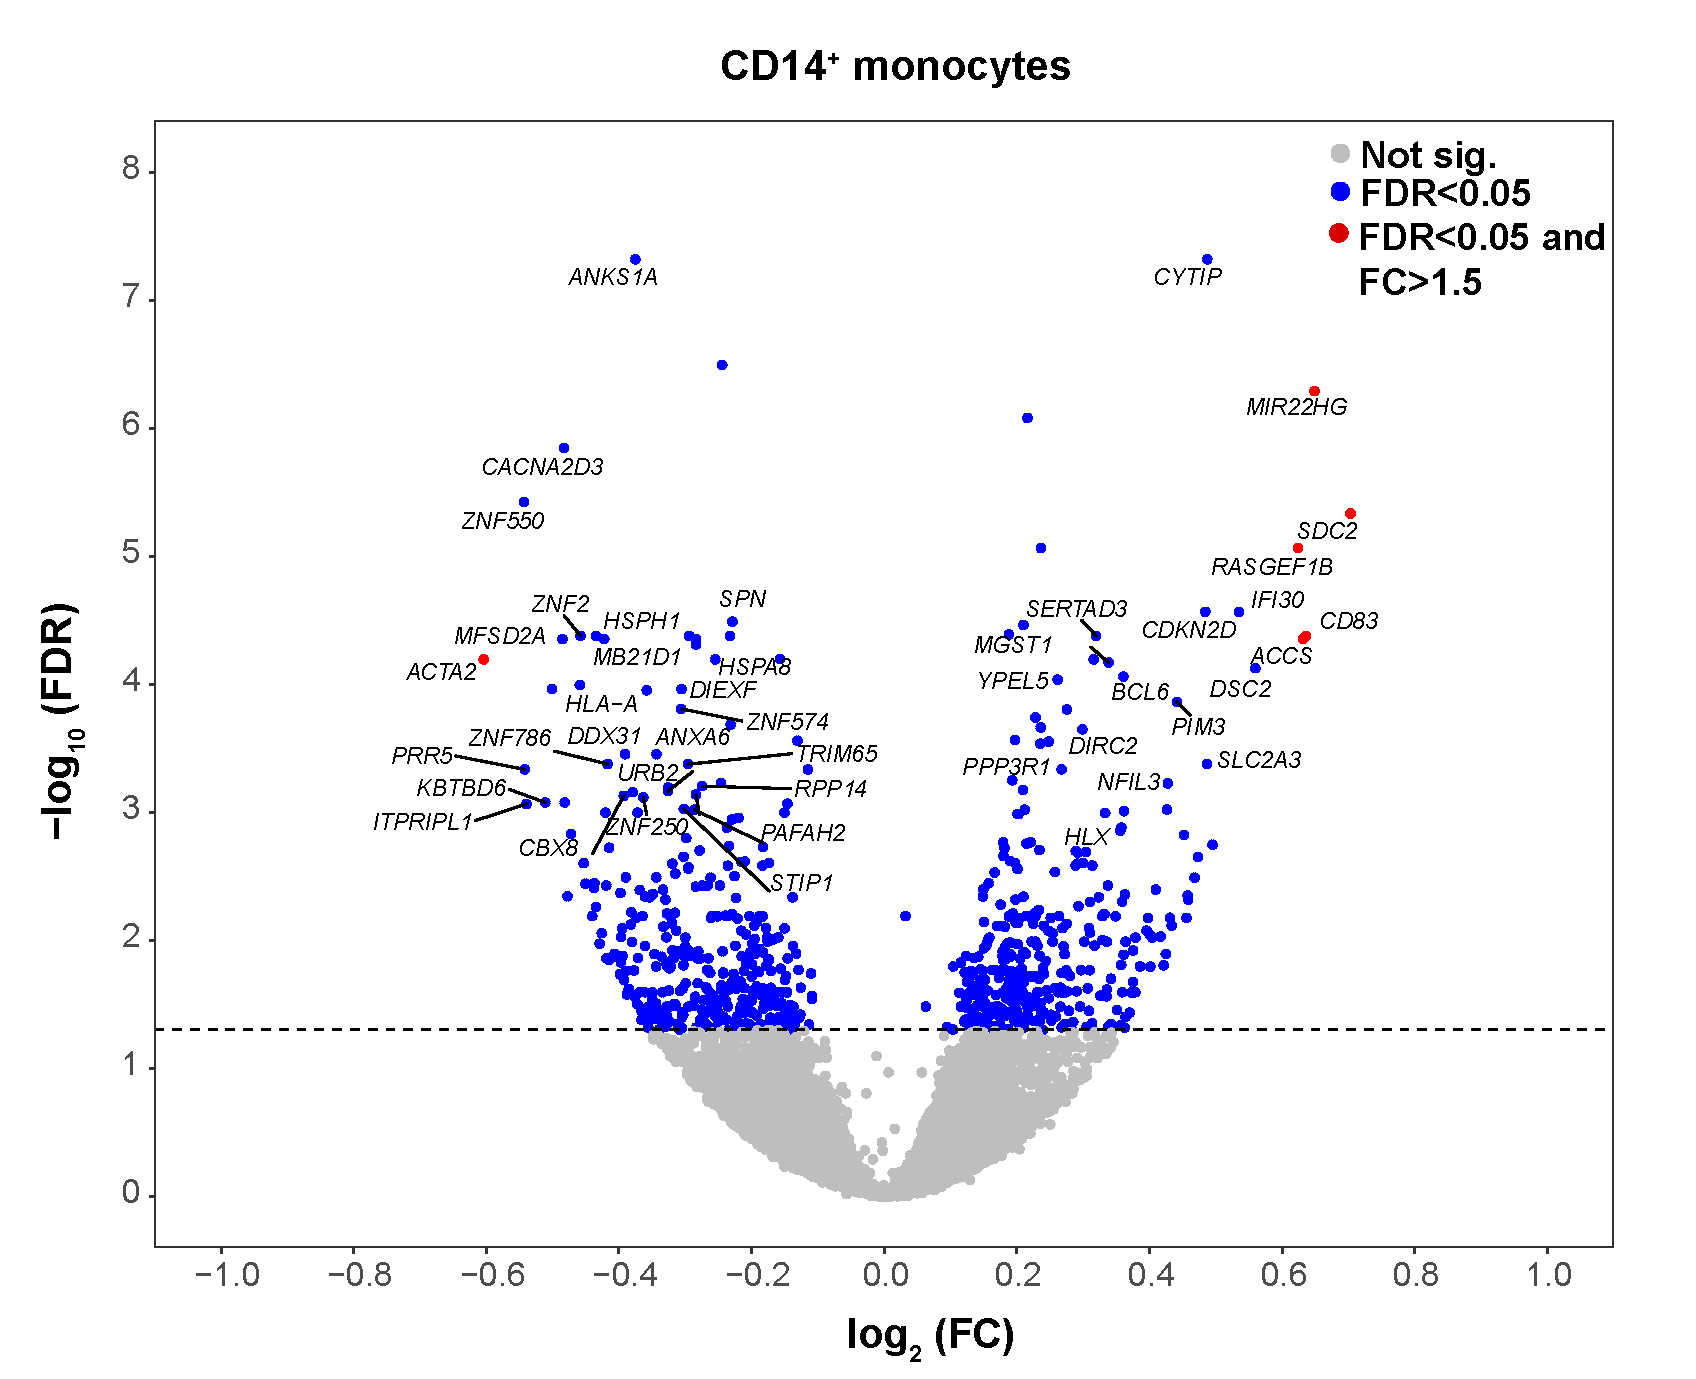
\includegraphics[width=\textwidth]{./Results2/pdfs/RNA_PS_CTL_CD14_volcano_plot}
\caption{\textbf{}}
% The percentage sign indicated that the other subfig goes side by side
\end{subfigure}%
\begin{subfigure}{0.5\textwidth}
\centering
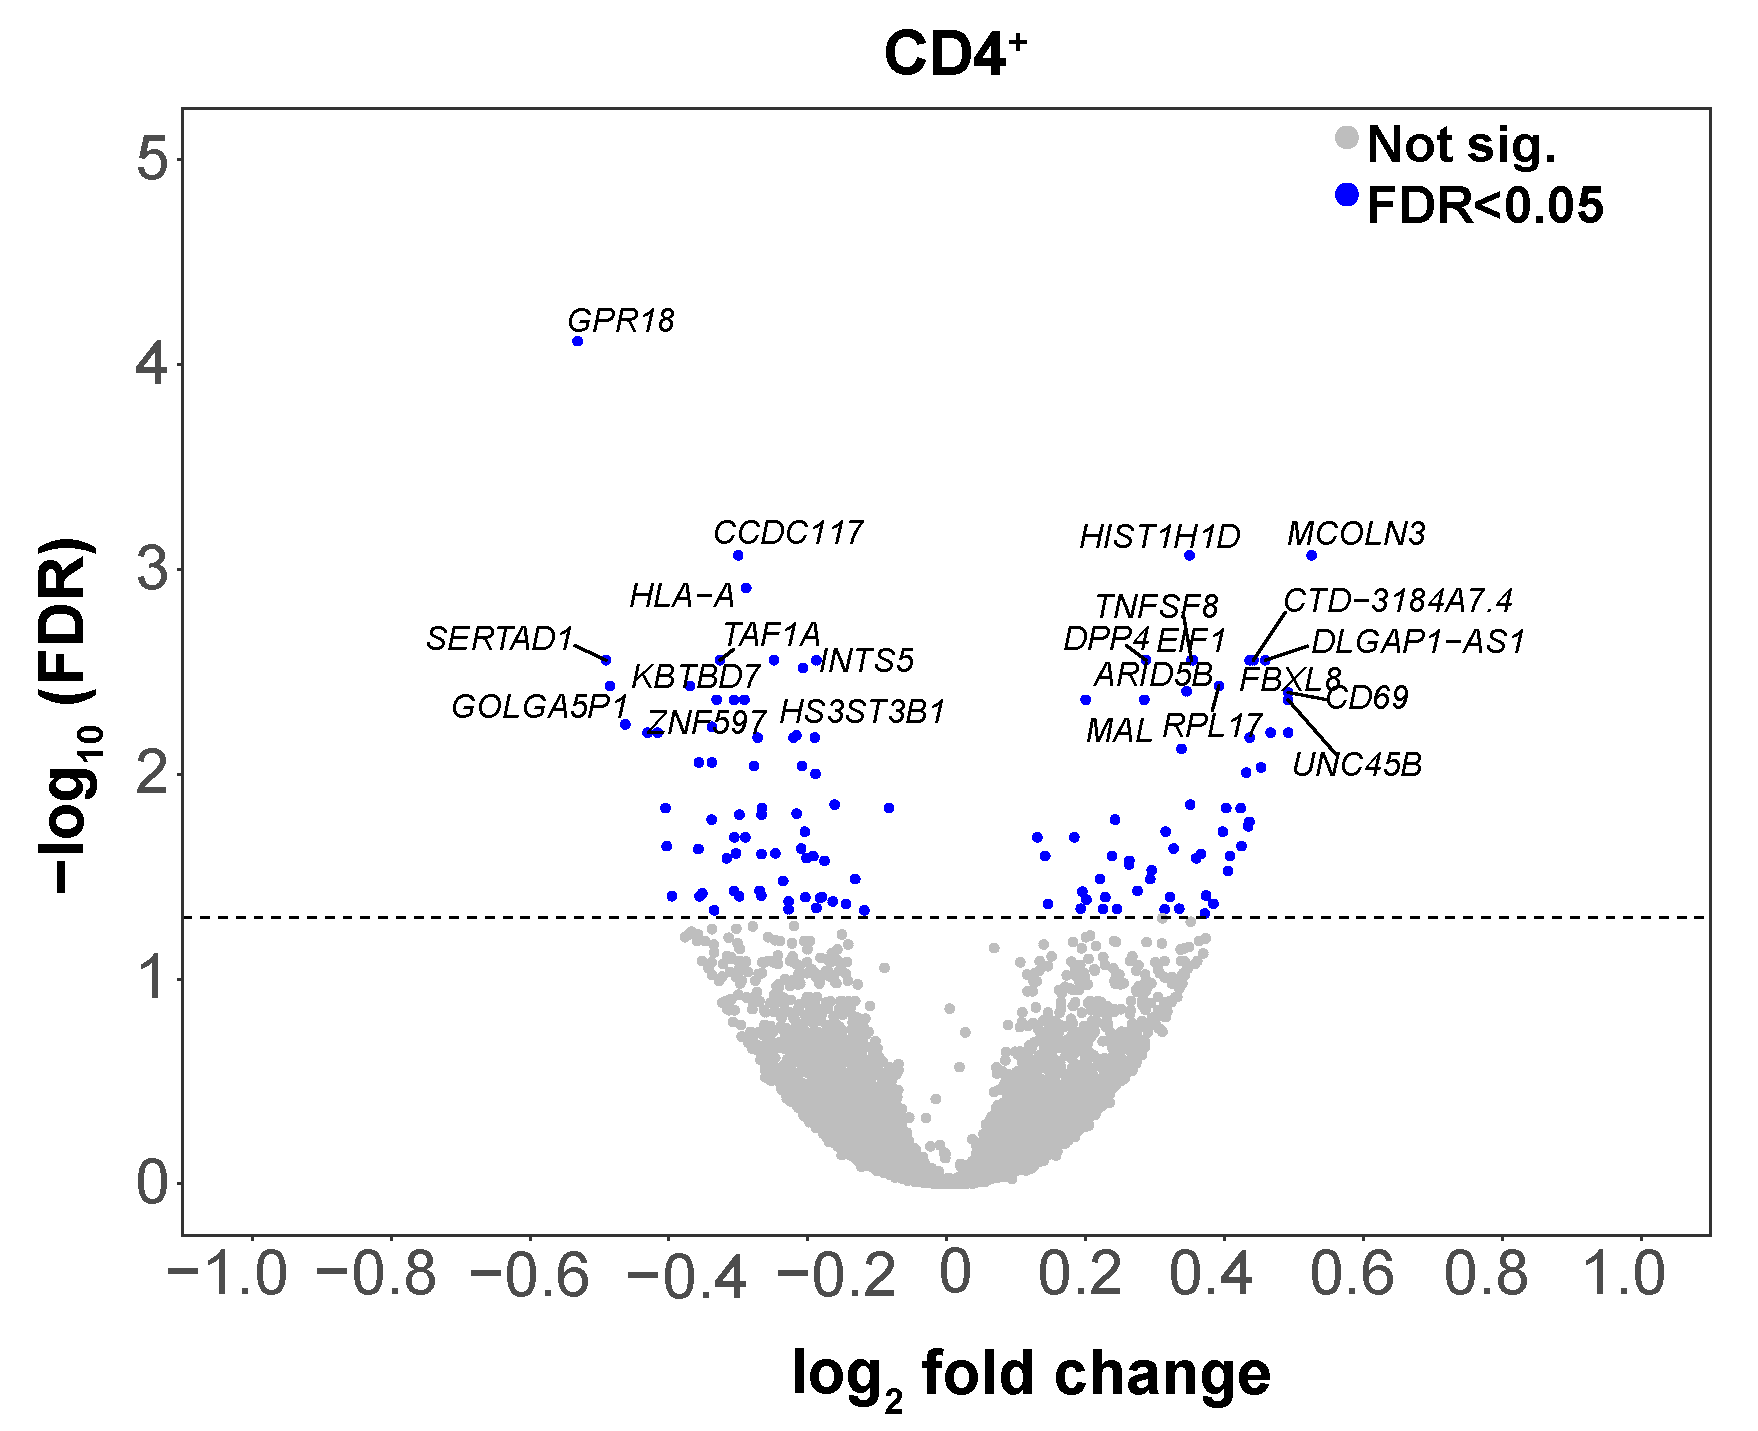
\includegraphics[width=\textwidth]{./Results2/pdfs/RNA_PS_CTL_CD4_volcano_plot}
\caption{\textbf{}}
\end{subfigure}
\begin{subfigure}{0.5\textwidth}
\centering
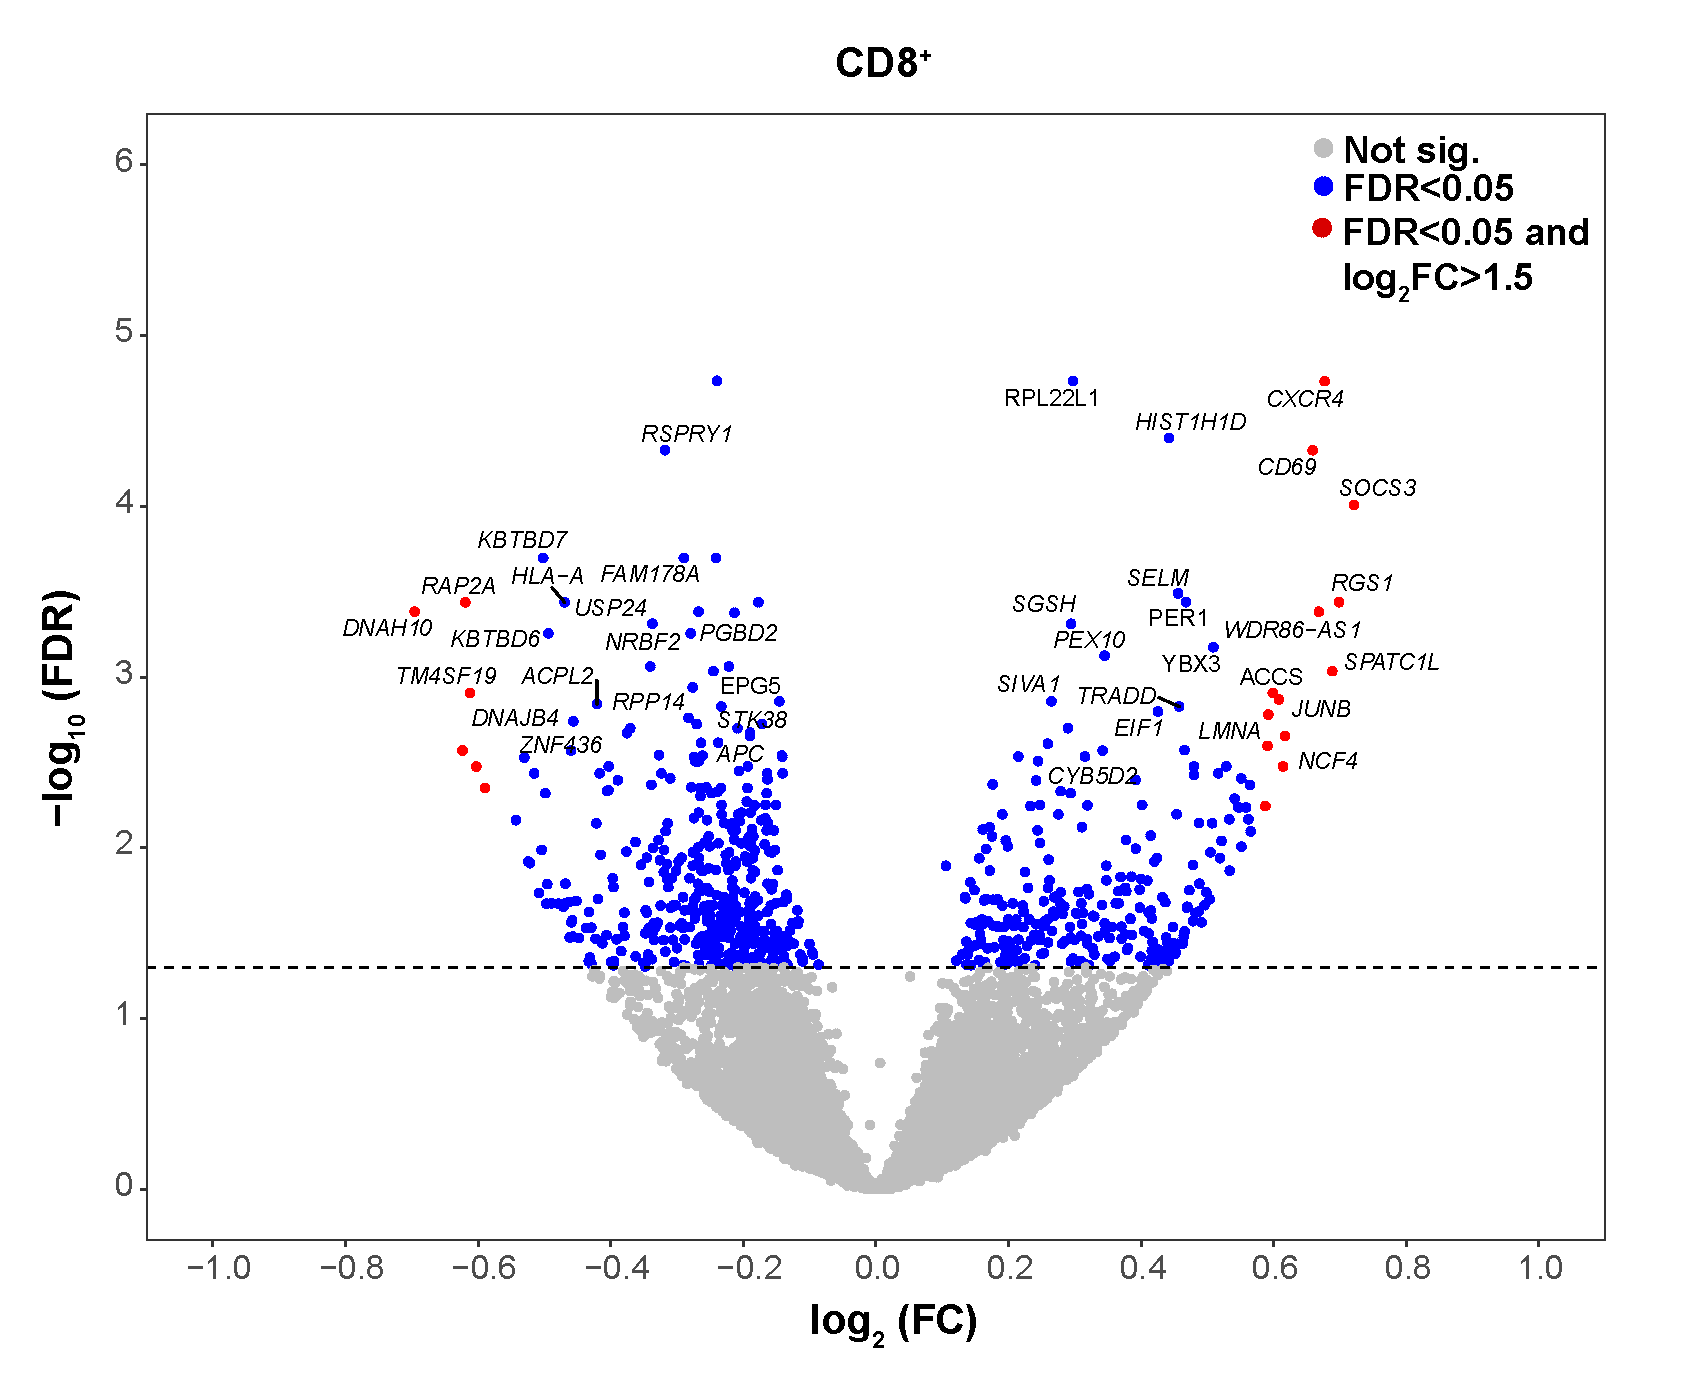
\includegraphics[width=\textwidth]{./Results2/pdfs/RNA_PS_CTL_CD8_volcano_plot}
\caption{\textbf{}}
% The percentage sign indicated that the other subfig goes side by side
\end{subfigure}%
\begin{subfigure}{0.5\textwidth}
\centering
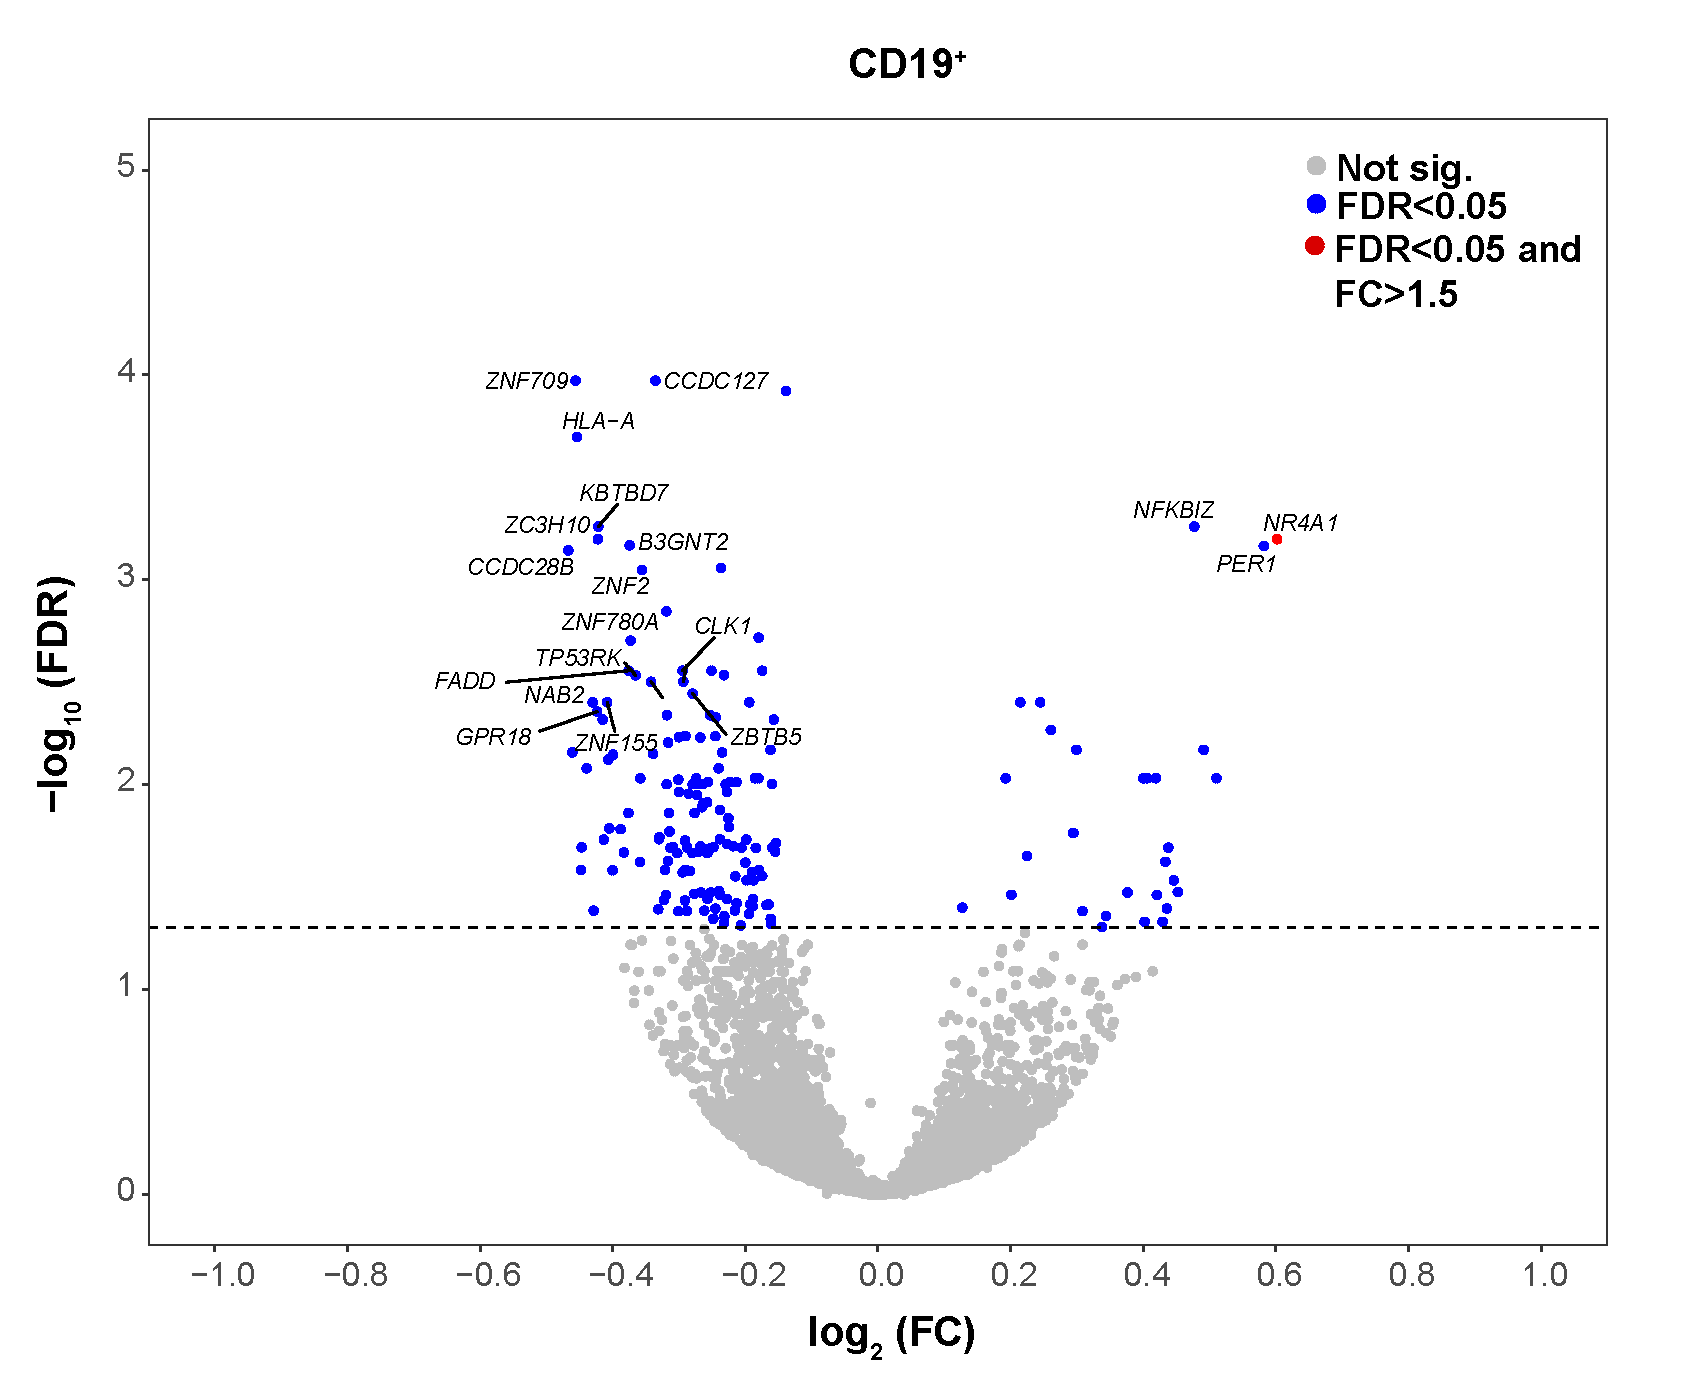
\includegraphics[width=\textwidth]{./Results2/pdfs/RNA_PS_CTL_CD19_volcano_plot}
\caption{\textbf{}}
\end{subfigure}
\caption[Magnitude and significance of the gene expression changes between psoriasis patients and healthy controls in four immune cell types.]{\textbf{Magnitude and significance of the gene expression changes between psoriasis patients and healthy controls in four immune cell types.} Volcano plots for the results of the DGE analysis in a) CD14$^+$ monocytes, b) CD4$^+$, c) CD8$^+$ and d) CD19$^+$ cells. For each gene, the log$_2$(FC) represents the change in expression for that gene in the psoriasis group with reference to the healthy controls. Significant DEGs (FDR$<$0.05) in blue for absolute FC $<$1.5 and red for absolute FC $>$1.5. The volcano plots include mRNAs and lncRNAs}
\label{figure:RNAseq_PS_CTL_volcano_plots}
\end{figure} 


Some of the DEGs across the four cell types overlapped some of the DEGs from the two most comprehensive studies comparing expressin of PBMCs isolated from psoriasis patients an healthy controls \parencite{Leo2009,Coda2012}. The greatest overlap (7 genes) was found between the DEGs in CD14$^+$ monocytes and those identified by Coda \textit{et al.}, 2012. However, 5 out of 7 presented opposite direction. One of those genes dysregulated in the same direction was ubiquitin conjugating enzyme E2 D1 (\textit{UBE2D1}), which mediates, for example, ubiquitination of the TNF receptor-associated factor 6 (TRAF6) protein \parencite{Gru2008}. The greatest overlap with the Lee and colleagues DEGs was found for CD8$^+$ cells (3 genes) in the same direction. For example, CDC like kinase 1 (\textit{CLK1}) involved in protein splicing was downregulated in this CD8$^+$ data set and in the Lee PBMCs in patients when compared to controls and its deficiency has been shown to lead to neuro-inflammation in mice \parencite{Gu2017}. Similarly, only one overlap was found with the psoriasis DEGs in a study comparing PBMCs transcriptional profiles of three inflammatory diseases (IBD, RA and psoriasis)\parencite{Mesko2010}. This was for the nicotinamide pPhosphoribosyltransferase (\textit{NAMPT}) gene involved in metabolism and stress response, which was up-regulated in our CD14$^+$ monocytes as well as in PBMCs from psoriasis, IBD and RA patients, suggesting its role as a marker of inflammation rather than marker for psoriasis.

In order to incorporate the psoriasis genetic information from GWAS studies, an overlap between the significant DEGs (FDR$<$0.05) across the four cell types and a list with the putative genes associated with psoriasis GWAS hits from the NHGRI-EBI catalog (https://www.ebi.ac.uk/gwas) curated to include other genes from more recent studies was performed (Table \ref{tab:RNAseq_PS_CTL_GWAS_overlap}). CD8$^+$ was the cell type with the largest number of DEGs (7 hits) overlapping with putative GWAS genes, followed by CD14$^+$ monocytes and CD4$^+$ (3 hits each). Some of those genes were found in more than one cell type, including \textit{NFKBIA}, \textit{TNFAIP3} and \textit{NFKBIZ}, amongst others.  

\begin{table}[htbp]
%\setlength{\tabcolsep}{20pt} only to stretch the columns if you want
%\renewcommand{\arraystretch}{1.5}
\centering
\begin{tabular}{@{} c c c c}
\toprule
\textbf{Cell type}   & \textbf{Number of GWAS}   & \textbf{Up-regulated}   & \textbf{Down-regulated}  \\
										 & \textbf{overlaps}         & \textbf{genes}          &\textbf{genes} \\
\midrule
\midrule
CD14$^+$             & 3  & \textit{NFKBIA}                                   & \textit{IL23A}, \textit{FASLG}\\                 
CD4$^+$              & 3  & \textit{TNFAIP3}, \textit{NFKBIZ}                 & \textit{FASLG} \\
CD8$^+$              & 7  & \textit{TNFAIP3}, \textit{NFKBIA}, \textit{ETS1}, & \textit{B3GNT2}, \textit{FASLG} \\ 
                     &    & \textit{SOCS1},\textit{NFKBIZ}                    &  \\ 
CD19$^+$             & 2  & \textit{NFKBIZ}                                   & \textit{B3GNT2}\\
\bottomrule 
\end{tabular}
\medskip %gap
\caption[Overlap between putative psoriasis GWAS genes and the reported significantly DEGs in CD14$^+$ monocytes, CD4$^+$, CD8$^+$ and CD19$^+$ cells.]{\textbf{Overlap between putative psoriasis GWAS genes and the reported significantly DEGs in CD14$^+$ monocytes, CD4$^+$, CD8$^+$ and CD19$^+$ cells.} DEGs list based on FDR$<$0.05.}
\label{tab:RNAseq_PS_CTL_GWAS_overlap}
\end{table}
\bigskip %bigger spac


\subsubsection{The role of lncRNAs in psoriasis circulating immune cells}
In addition to protein coding genes, some of the DEGs identified were classified as lncRNAs. Total CD8$^+$ and CD14$^+$ monocytes were the two cell types presenting the largest number of dysregulated lncRNAs between psoriasis patients and controls (Table \ref{tab:RNAseq_PS_CTL_differential_analysis_results}. In contrast, CD19$^+$ was the cell type showing the lower number of lncRNAs differentially expressed. The vast majority of the dysregulated lncRNAs between patients and controls at FDR$<$0.05 were functionally uncharacterised, difficulty the interpretation of these results. 

Amongst the known ones in CD14$^+$ monocytes, the negative regulator of antiviral response \textit{DYNLL1-AS1} (or \textit{NAV}) which has been shown to affect the histones modifications of some critical IFN-stimulated genes (ISGs), such as \textit{IFITM3} and \textit{MxA} leading to down-regulation of their expression \parencite{Ouyang2014}. In this data, \textit{DYNLL1-AS1} was down-regulated indicating lack of one of the negative regulators of the IFN response, regardless the reverse IFN-$\gamma$ signature observed in the pathway enrichment analysis. Another interesting dysregulated lncRNA in CD14$^+$ monocytes was the HOXA transcript antisense RNA myeloid-specific 1\textit{HOTAIRM1}.In a study using PsA PBMCs \textit{HOTAIRM1} was found to be down-regulated and connected to the expression of the RNA helicase and ATPase \textit{UPF1} \ref{Dolcino2018}. \textit{UPF1} is involved in the the nonsense‐mediated decay and in partnership with the monocyte chemotactic protein-1-induced protein-1 (\textit{MCPIP1}) gene driven degradation of inflammation-related mRNAs to ensure maintenance of the homeostasis \parencite{Mino2015}. In this present study, \textit{HOTAIRM1} appeared to be up-regulated in the CD14$+$ monocytes from psoriasis patients (Figure \ref{figure:RNAseq_PS_CTL_CD14_expression_HOTAIRM_UPF1} a) and this was consistent with significant down-regulation of \textit{UPF1} in the same cell type (Figure \ref{figure:RNAseq_PS_CTL_CD14_expression_HOTAIRM_UPF1} b), suggesting impairment of this homeostatic mechanisms in the psoriasis patients. 



\begin{figure}[htbp]
\centering
\begin{subfigure}{0.5\textwidth}
\centering
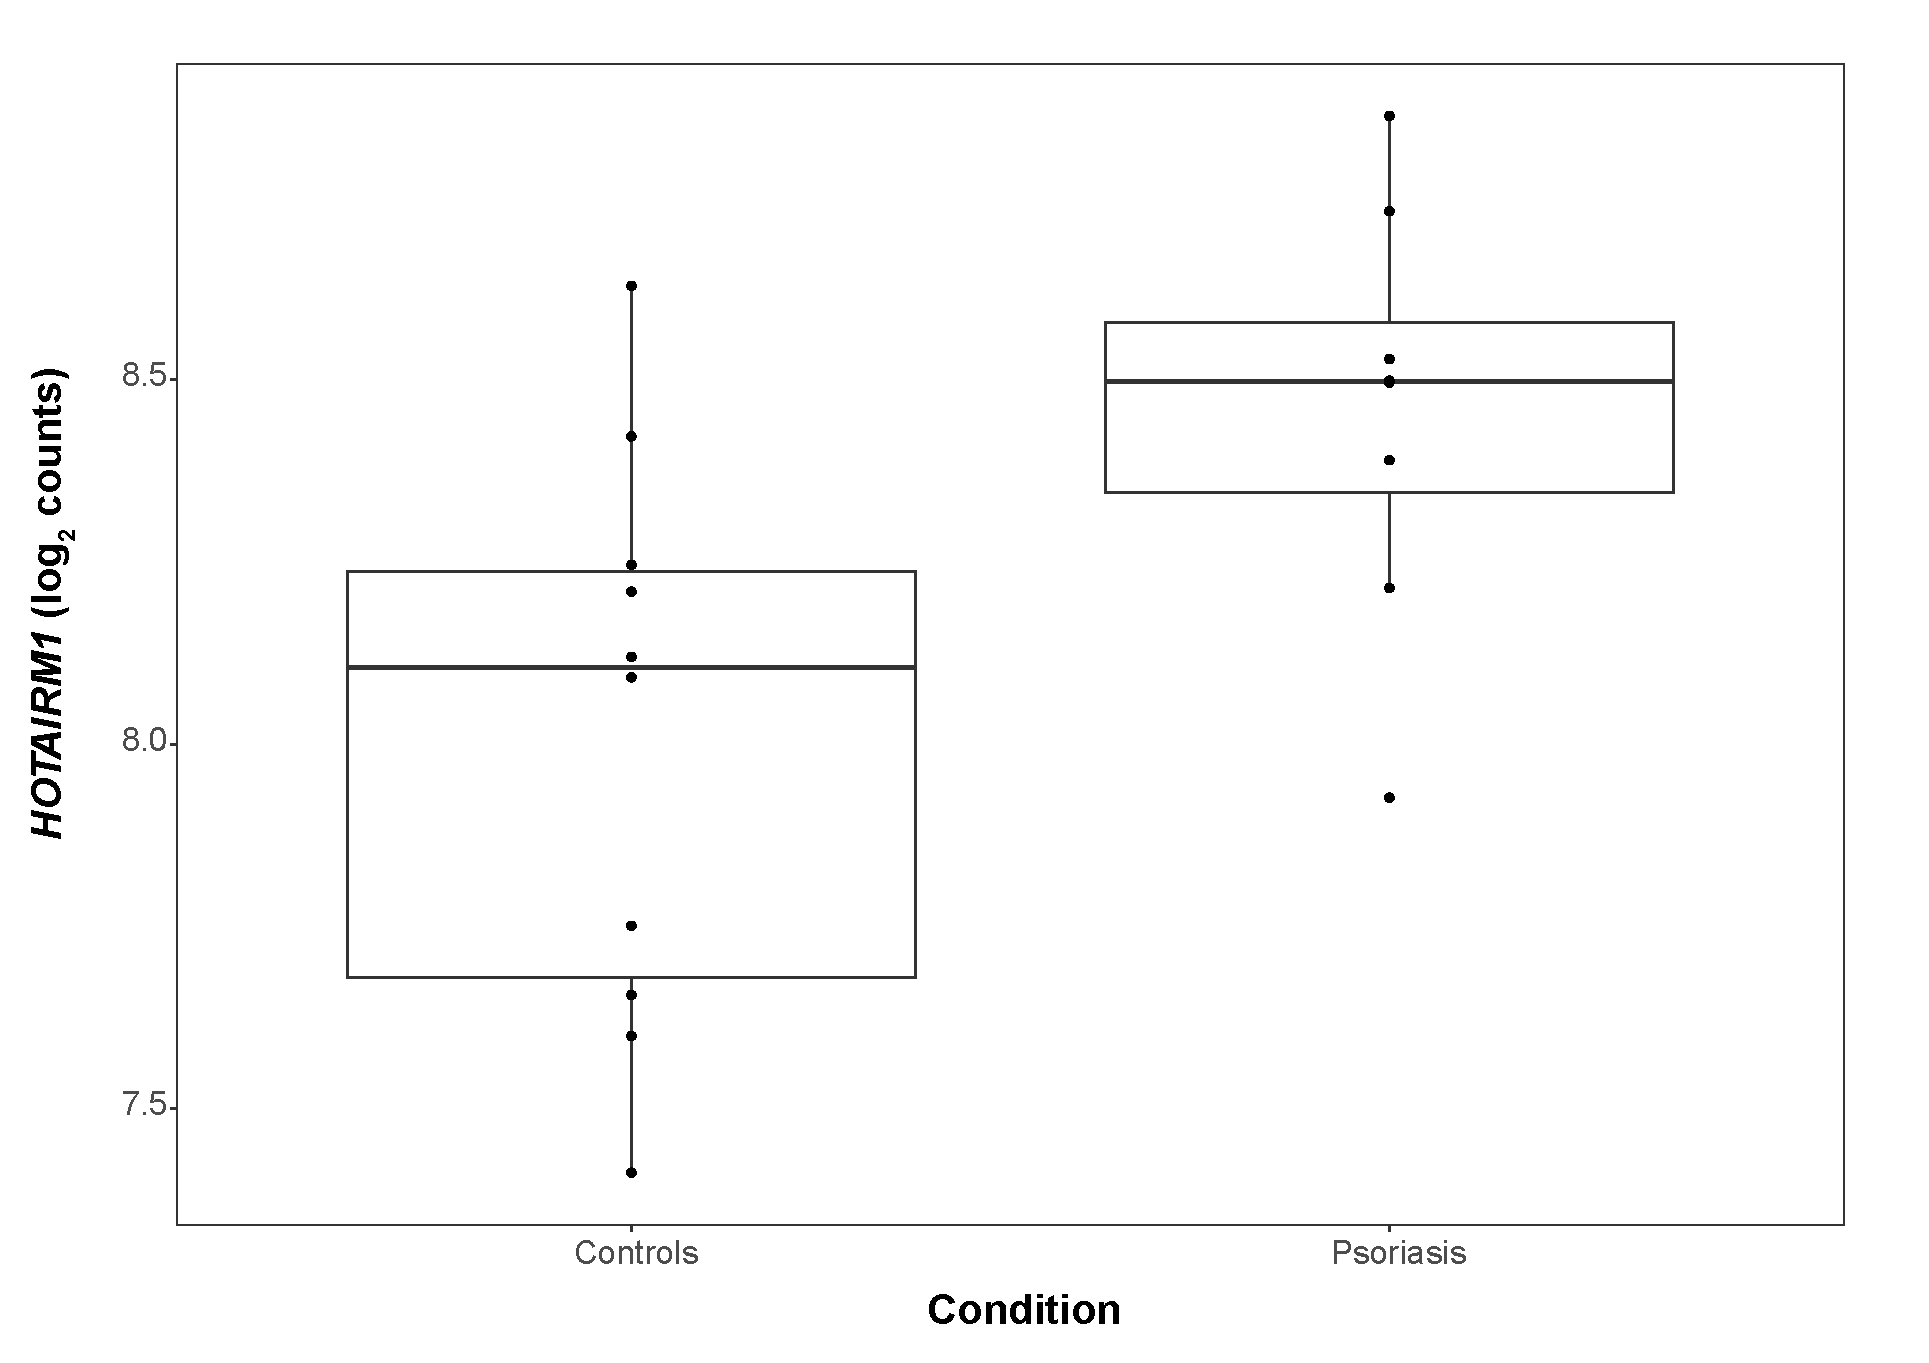
\includegraphics[width=\textwidth]{./Results2/pdfs/RNAseq_PS_CTL_lncRNA_HOTAIRM1_CD14}
\caption{\textbf{}}
% The percentage sign indicated that the other subfig goes side by side
\end{subfigure}
\begin{subfigure}{0.5\textwidth}
\centering
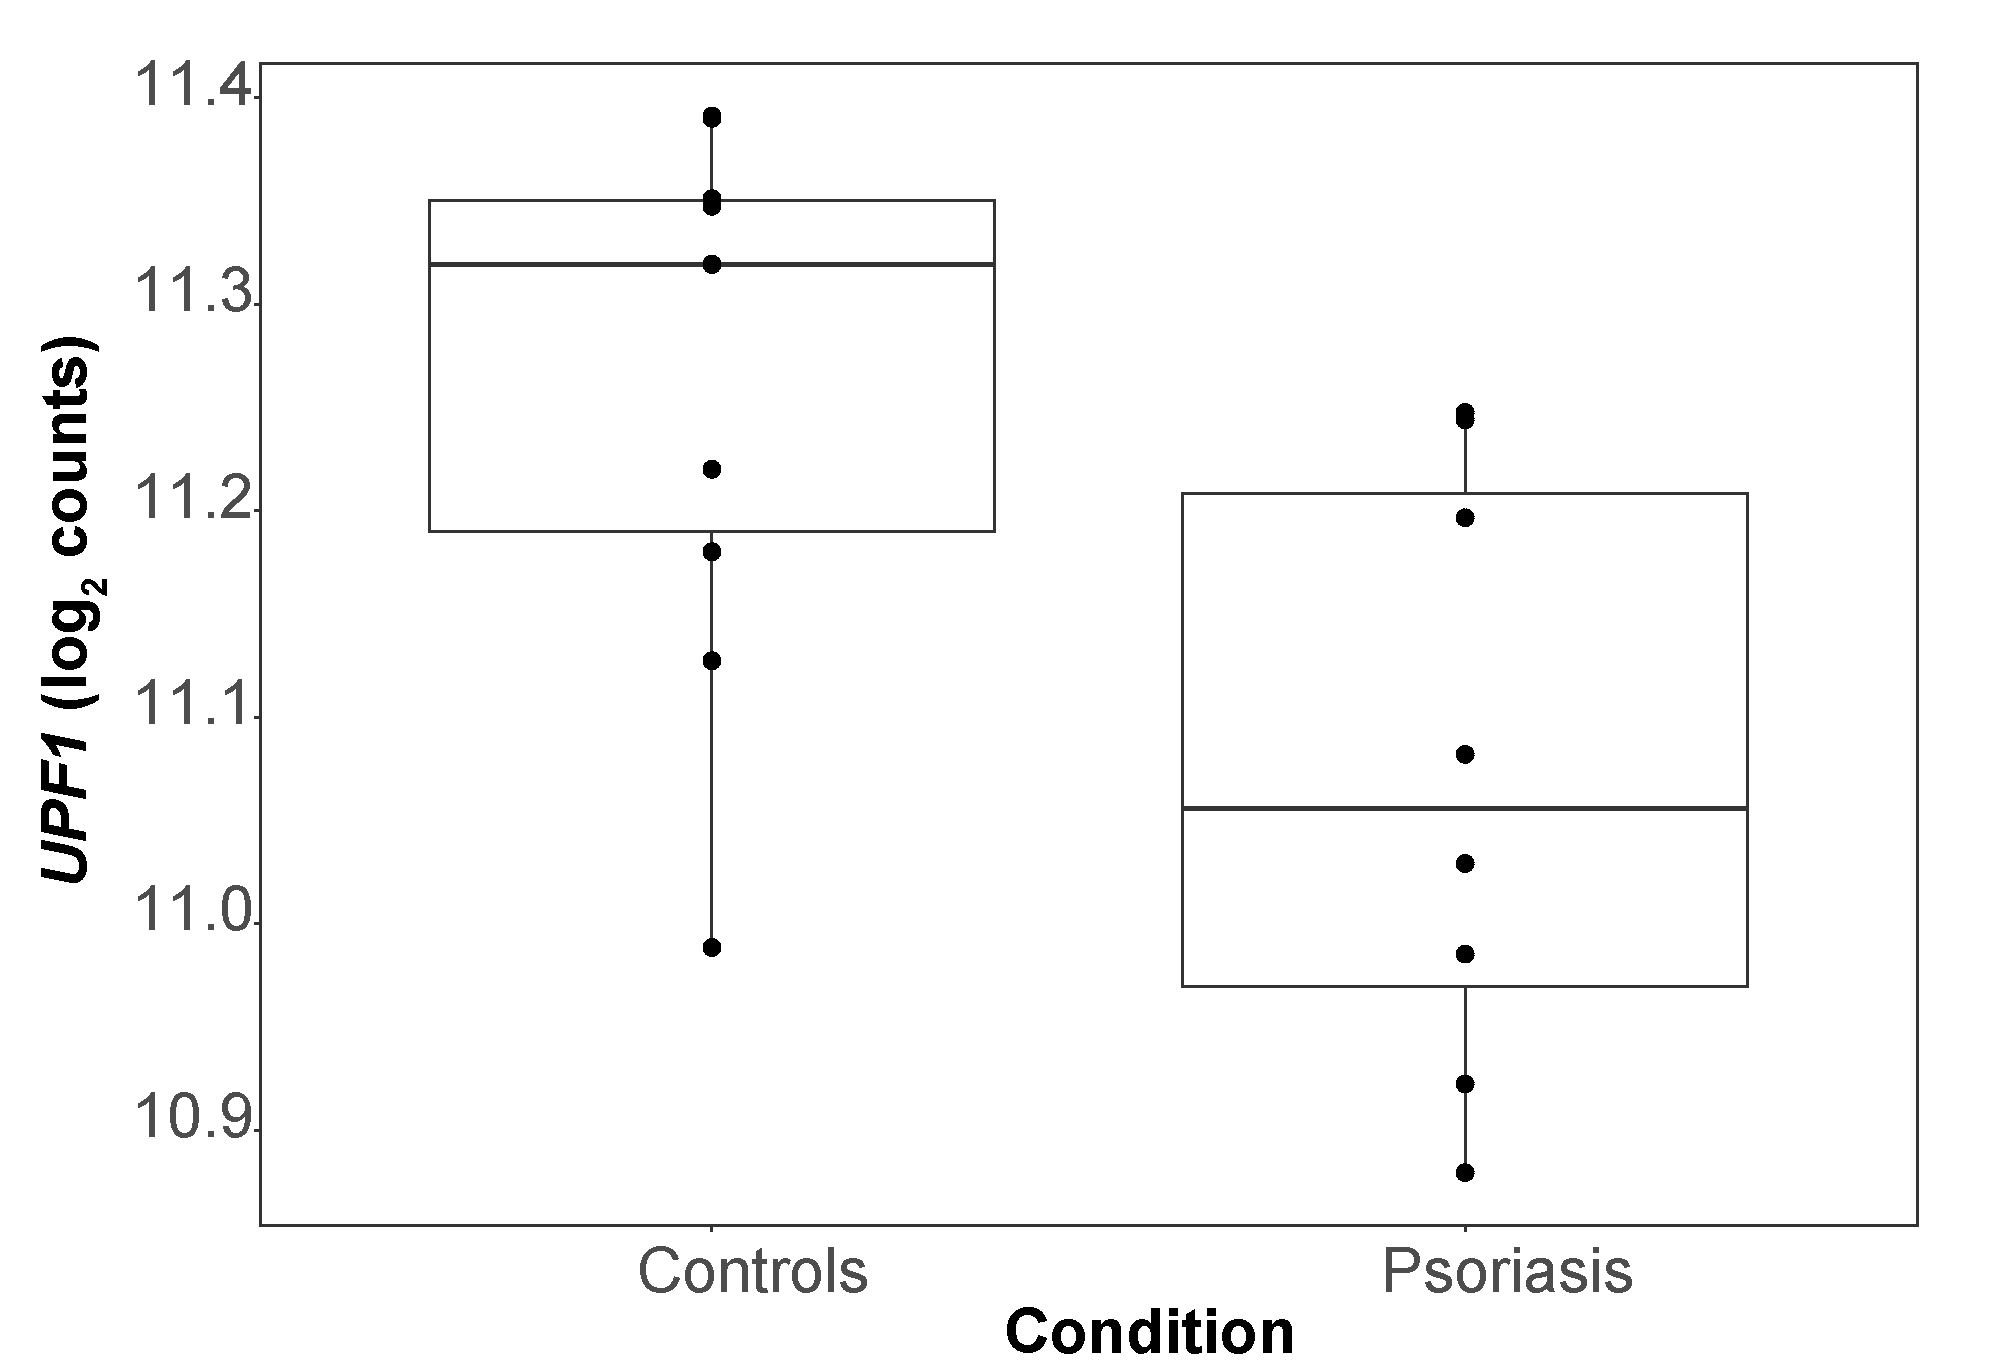
\includegraphics[width=\textwidth]{./Results2/pdfs/RNAseq_PS_CTL_lncRNA_UPF1_CD14}
\caption{\textbf{}}
\end{subfigure}
\caption[RNA-seq expression levels of the lncRNA \textit{HOTAIRM1} and its putative target UPF1 in psoriasis and healthy controls CD14$^+$ monocytes.]{\textbf{RNA-seq expression levels of the lncRNA \textit{HOTAIRM1} and its putative target UPF1 in psoriasis and healthy controls CD14$^+$ monocytes.} Expression is illustrated as the log$_2$ of the normalised read counts mapping to a) the lncRNA \textit{HOTAIRM1} and b)\textit{UPF1}, which as been identified as one of the putative genes regulated by this lncRNA in the study conducted by Dolcino \textit{et al.}, 2018.}
\label{figure:RNAseq_PS_CTL_CD14_expression_HOTAIRM_UPF1}
\end{figure} 


The last relevant lncRNA differentially expressed in monocytes was \textit{NEAT1}, which was up-regulated in the patients group when compared to the controls. \textit{NEAT1} has been reported to to also be up-regulated in SLE CD14$^+$ monocytes and knocking it down has revealed impairment of the TLR-4 signalling and down-regulation of inflammatory genes including IL-6 and CXCL10, amongst others \parencite{Zhang2016}.

For total CD8$^+$ cells, the most relevant non-coding RNA was the miR \textit{MIR146A}, which was captured in the standard RNA library preparation . Interestingly, \textit{MIR146A} expression was down-regulated in psoriasis patients when compared to controls. This is in line with findings in serum from SLE and early RA patients \parencite{Wang2012,Filkov\'{a}}. In contrast, trancriptomic studies using PBMCs from plaque psoriasis and also similar studies in RA (including PBMCs, SFMCs and CD4$^+$ isolated from both tissues, amongst others) have reported increased levels of miR-146a in patients when compared to controls \parencite{Ele-Refaei2015,Churov2015}. Molecular studies have suggested the role on miR-146a as a negative regulator of the TLR-4 pathway \parencite{Taganov2006}. This study demonstrated regulation of \textit{MIR146A} expression by NF-$\kappa$B upon inflammation as well as \textit{in vitro} targeting of the 3'UTR from \textit{TRAF6} and IL-1 receptor-associated kinase 1 (\textit{IRAK1}) genes. These are adaptor molecules that lead to activation of kinases from the TLR-4 pathway that eventually lead to translocation of NF-$\kappa$B and AP-1 into the nucleus and transcriptional up-regulation of inflammatory genes. 

Other lncRNAs were found to be dyregulated in more than one cell type. For example, \textit{KCNQ1OT1} was downregulated in both, CD4$^+$ and CD8$^+$ cells. Dysregulated expression of this lncRNA has been reported in the Beckwith-Wiedemann syndrome consisting of a loss-of-imprinting pediatric overgrowth disorder with some skin features such as creases or pits in the skin near the ears \parencite{Pandei2008}. \textit{KCNQ1OT1} has been reported to interact with DNA methyltransferases and also to facilitate the interaction of these enzymes with the chromatin, leading to misregulation of imprinted loci.


\subsubsection{Pathway enrichment analysis for the DEGs}

In order to better understands the biological role of the significantly modulated genes, pathway enrichment analysis was performed for each cell type. The ATAC-seq results and the moderated FCs in the DGE analysis illustrated in the volcano plots suggest that the differences between patients and controls in these circulating immune cells are moderate. However, moderate differences may have an important impact in their phenotype for infiltration and activation in the skin. Therefore, to avoid losing biological meaningful effects and have a better understanding of the affected pathways, genes with FDR$<$0.05 and no FC cut off were included in this analysis. Functionally relevant significantly enriched pathways (FDR$<$0.01) were revealed for CD14$^+$ monocytes and CD8$^+$ (Table \ref{tab:tab:RNAseq_PS_CTL_pathway_enrichment} and \ref{tab:RNAseq_PS_CTL_additional_pathways}). In CD19$^+$ cells, only one pathway named as generic transcription appeared to be significantly enriched for DEGs in this cell type. In contrast, in CD4$^+$ cell no pathway was enriched for modulated genes, consistently with the fact that this cell type presented the most moderate signature of disease modulated genes. 

\begin{table}[htbp]
%\setlength{\tabcolsep}{20pt} only to stretch the columns if you want
%\renewcommand{\arraystretch}{1.5}
\centering
\begin{tabular}{@{} c c}
\toprule
\textbf{Cell type} & \textbf{Pathways} \\
\midrule
\midrule
                      & MAPK signalling \\
                      & IL-12 mediated signaling events \\
				              & Th-1 and Th-2 cell differentiation \\
CD14$^+$ monocytes    & Th-17 cell differentiation \\
				              & TCR signalling \\
				              & Platelet-derived growth factor (PDGF-$\beta$) signalling\\
				              & Forkhead box O (FoxO) signalling \\
\midrule				
CD8$^+$  & Osteoclast differentiation \\
         & MAPK signalling \\
				 & TNF signalling \\
         & IL-12 mediated signalling events \\
				 & NF-$\kappa$B signalling \\
				 & Chemokine signalling \\
\bottomrule
\end{tabular}
\medskip %gap
\caption[Most relevant pathways enriched for DEGs between psoriasis patients and healthy controls in CD14$^+$ monocytes and CD8$^+$ cells.]{\textbf{Most relevant pathways enriched for DEGs between psoriasis patients and healthy controls in CD14$^+$ monocytes and CD8$^+$ cells.} The enrichment analysis was conducted using significantly DEGs FDR$<$0.05 and no FC threshold. Enriched pathways had FDR$<$0.01 and a minimum of ten gene members overlapping with DEGs for that particular cell type.}
\label{tab:RNAseq_PS_CTL_pathway_enrichment}
\end{table}

Amongst the relevant pathways, MAPK signalling enrichment was shared between CD14$^+$ monocytes and CD8$^+$ cells. Some of the DEGs contributing to the enrichment of this pathway in both cell types included MAPK gene members such as \textit{MAP3K4} and \textit{MAPK14}, both down-regulated in psoriasis when compared to controls. Interestingly, the MAP3K4 is a member of the MAPKKK family which expression is down-regulated in LPS-stimulated PBMCs from CD patients, leading to reduced expression of the cytokine \textit{IL-1A} and a relative immune deficiency in TLR-mediated cytokine production. Contributing to the enrichment \parencite{Kraan2012}. Moreover, DGE of members of the dual-specificity phosphatases (DUSP) family involved in the immune response fine-tuning \parencite{Qian2009} in the enrichment of the MAPK pathway in CD14$^+$ monocytes and CD8$^+$ cells. \textit{DUSP10} was down-regulated in the psoriasis CD14$^+$ monocytes and could be modulating reactive oxygen species production according to a knock-out mice phenotype presenting enhanced inflammation \parencite{Qian2009}. Conversely, \textit{DUSP4} presented up-regulation in patients when compared to healthy controls and it could represent a pro-inflammatory feature as this gene has been demonstrated to have a role in driving inflammation in a sepsis mice model \parencite{Cornell2010}.  

Other interesting pathways enriched for both cell types DEGs IL-12 mediated signalling (Table \ref{tab:RNAseq_PS_CTL_pathway_enrichment}). IL-12 signalling leads to T cells proliferation and IFN-$\gamma$ production through activation of TFs from the STAT family, importantly STAT4and is also a well known drug target for psoriasis treatment. Interestingly, CD14$^+$ monocytes from psoriasis presented down-regulation of \textit{STAT4} and \textit{STAT5A} in patients compared to controls. Likewise, \textit{IFNG} expression in psoriasis patients was lower than in healthy controls in CD8$^+$ cells. This phenomenon has been previously observed in macrophages derived from AS patients as well as in an SpA rat model \parencite{Smith2008,Fert2014}. Additionally, \textit{IL2RA} was up-regulated in CD8$^+$ from psoriasis patients when compared to controls which may enhance formation of the IL2-R$\alpha$ and the signalling by this cytokine involved in effector and regulatory T cell differentiation \parencite{Malek2010}.


The platelet-derived growth factor (PDGF-$\beta$) signalling pathway was only enriched in CD14$^+$ monocytes (Table \ref{tab:RNAseq_PS_CTL_pathway_enrichment}). Within this pathway the \textit{SLA} gene appeared to be down-regulated in psoriasis patients compared to controls. A \textit{SLA} knock-out mice model have shown impaired IL-12 and TNF-$\alpha$ and failure of T cell stimulation by GM-CSG treated bone marrow-derived DCs \parencite{Liontos2011}.
%https://www.ncbi.nlm.nih.gov/pmc/articles/PMC3884931/
% role of SLA in monocytes http://www.jimmunol.org/content/186/4/1923.long

A number of very relevant inflammatory pathways in psoriasis were identified to be enriched only in CD8$^+$ cells. These included TNF, NF-$\kappa$B and chemokine signalling (Table \ref{tab:RNAseq_PS_CTL_pathway_enrichment}). Due to the close relationship between these three pathways, some DEGs contributed to the enrichment of more than one of them. For example, the NF-$\kappa$B inhibitor A (\textit{NFKBIA}) gene, which was up-regulated in CD8$^+$ cells from psoriasis compared to healthy controls, was present in all three pathways (Figure \ref{figure:RNAseq_PS_CTL_CD8_TNF_and_chemokine_pathway_modified} a). Another example was the TNF-$\alpha$ induced protein 3 (\textit{TNFAIP3}), also up-regulated, and a member of the TNF and NF-$\kappa$B pathways (fig). Interestingly, \textit{NFKBIA} and \textit{TNFAIP3} were also up-regulated in CD14$^+$ monocytes and CD4$^+$ cells. \textit{NFKBIA} gene code for the NF-$\kappa$B inhibitor alpha (I$\kappa$B$\alpha$) which binds to the NF-$\kappa$B subunits preventing them from translocation to the nucleus by masking a nuclear localization signal (NLS). Similarly, \textit{TNFAIP3} gene code for the zinc finger protein and ubiqitin-editing enzyme A20, that inhibits both NF-$\kappa$B signalling and TNF-mediated apoptosis. Unexpectedly, these two genes with an anti-inflammatory role appeared to be up-regulated in psoriasis patients when compared to controls in two of the studied cell types. 


\begin{figure}[htbp]
\centering
\begin{subfigure}{0.5\textwidth}
\centering
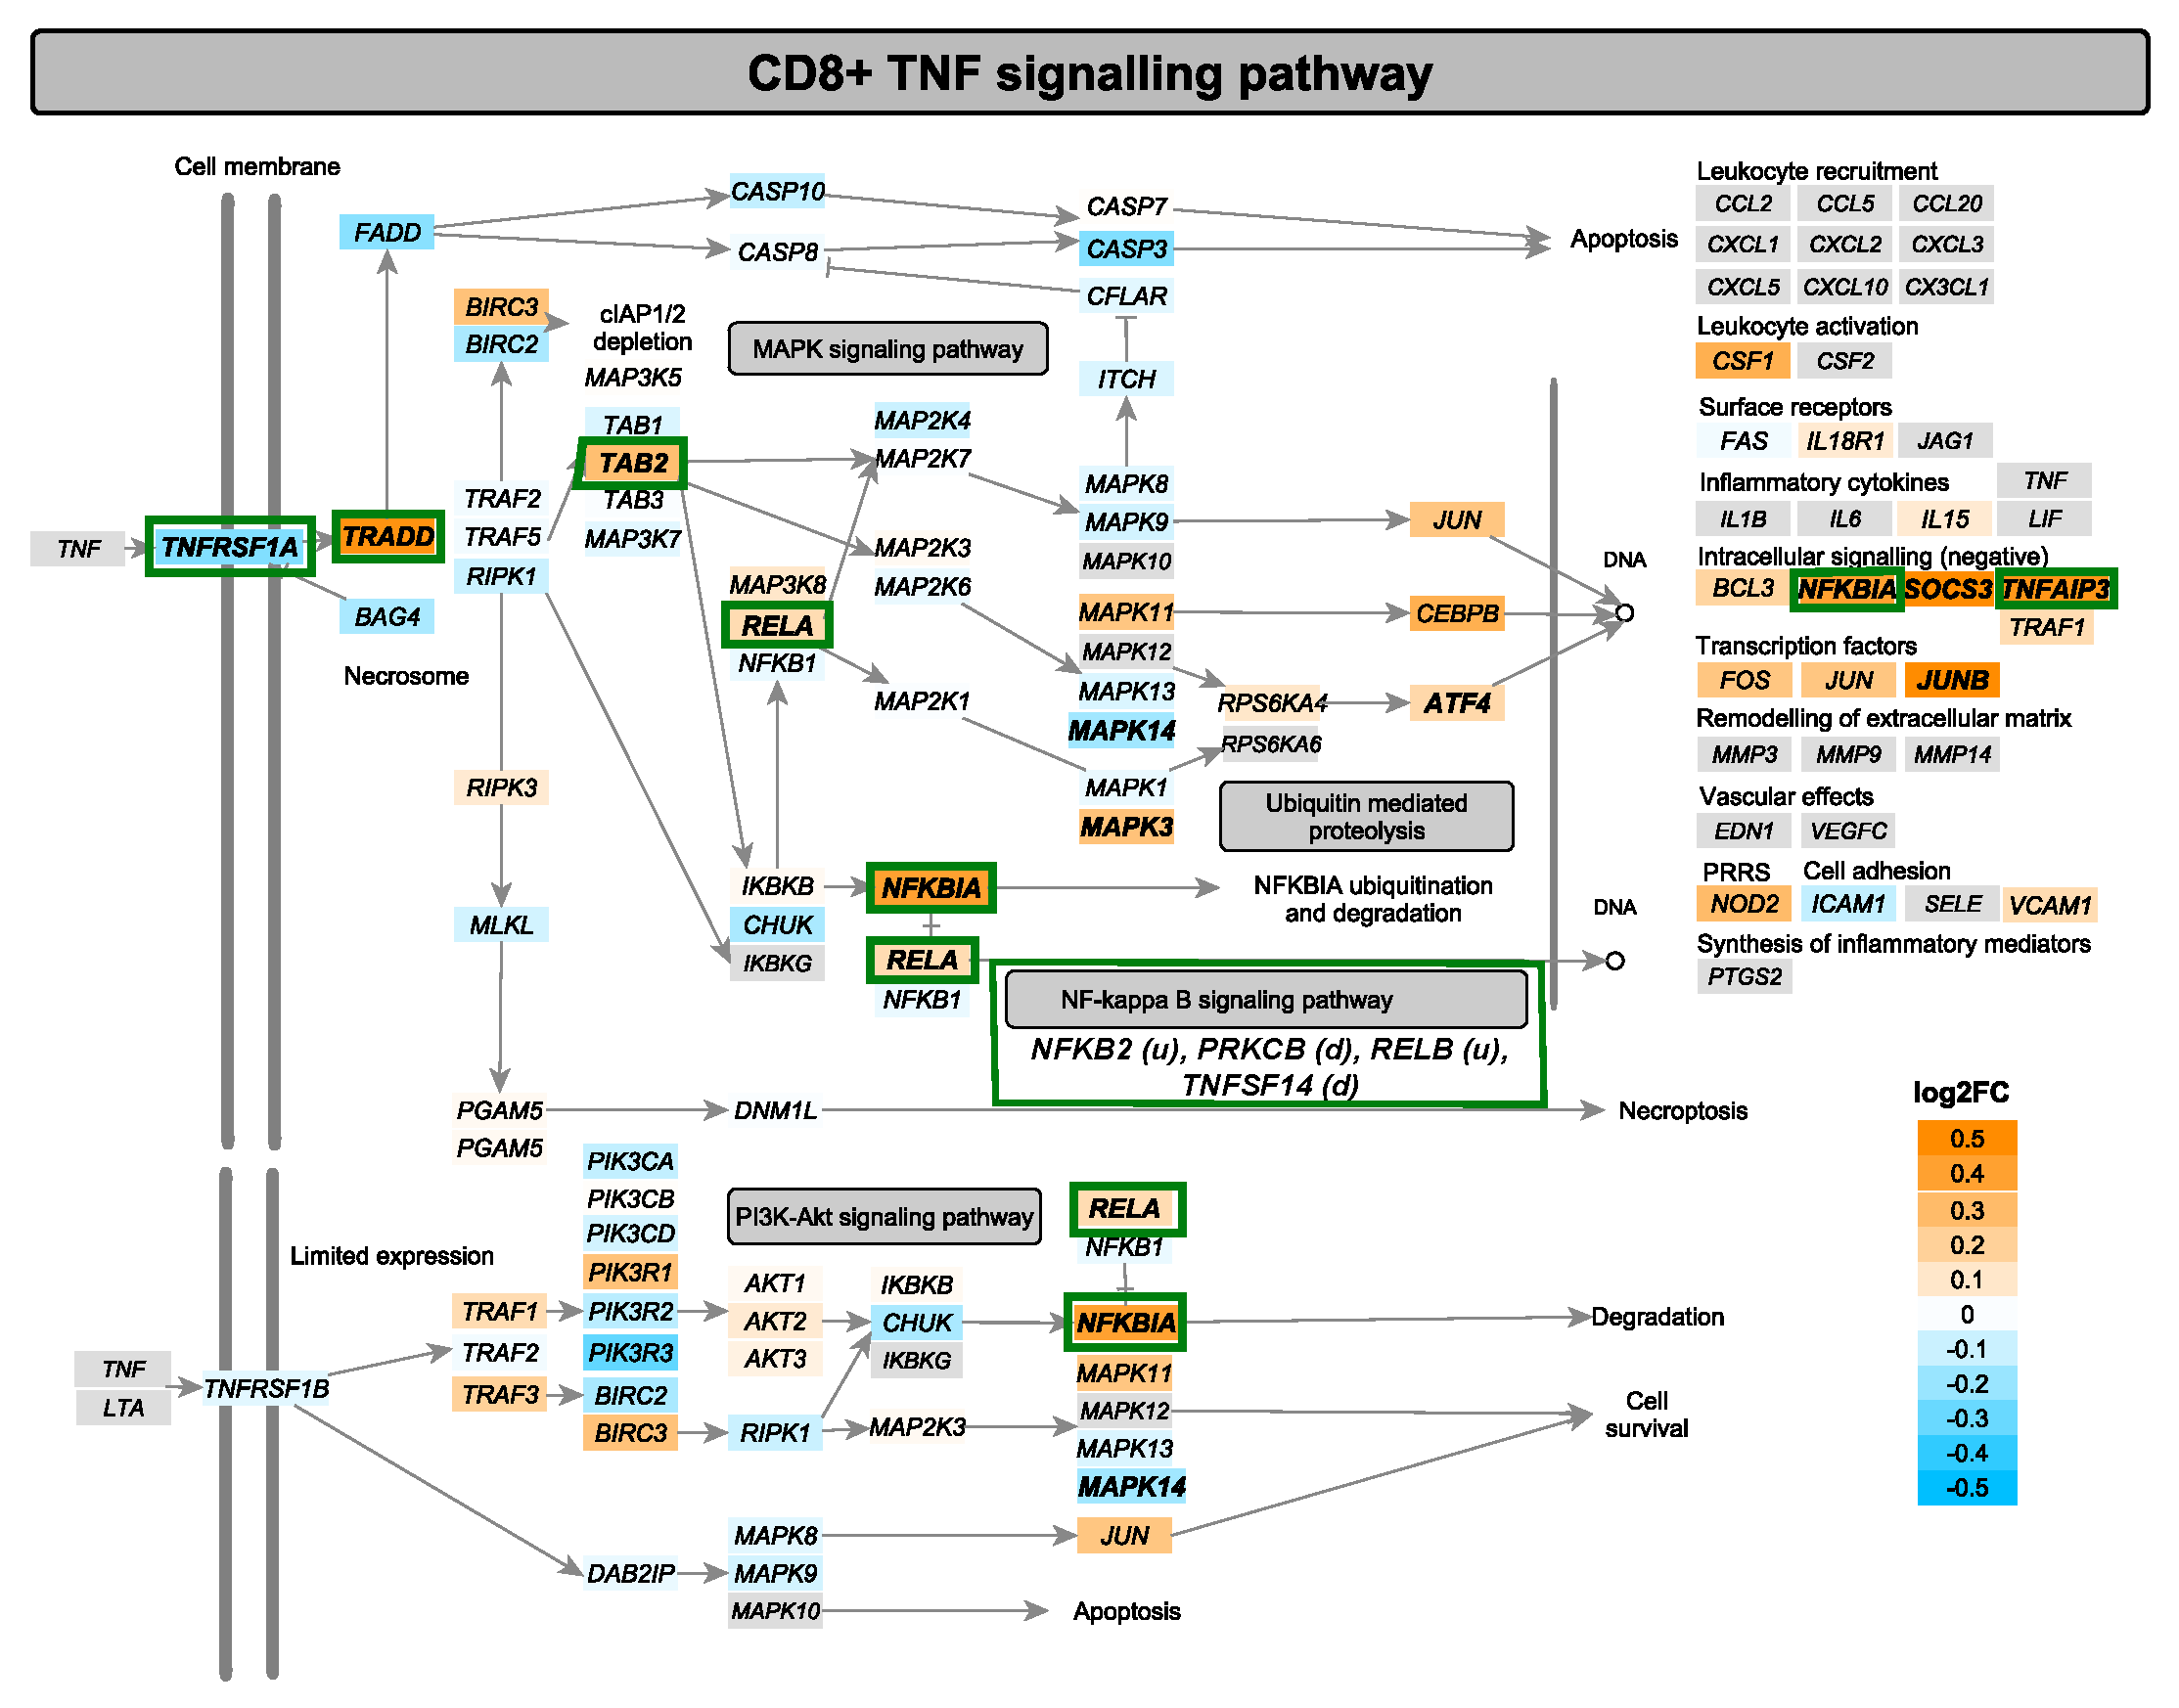
\includegraphics[width=\textwidth]{./Results2/pdfs/PS_CTL_CD8_all_TNF_pathway}
\caption{\textbf{}}
% The percentage sign indicated that the other subfig goes side by side
\end{subfigure}
\begin{subfigure}{0.5\textwidth}
\centering
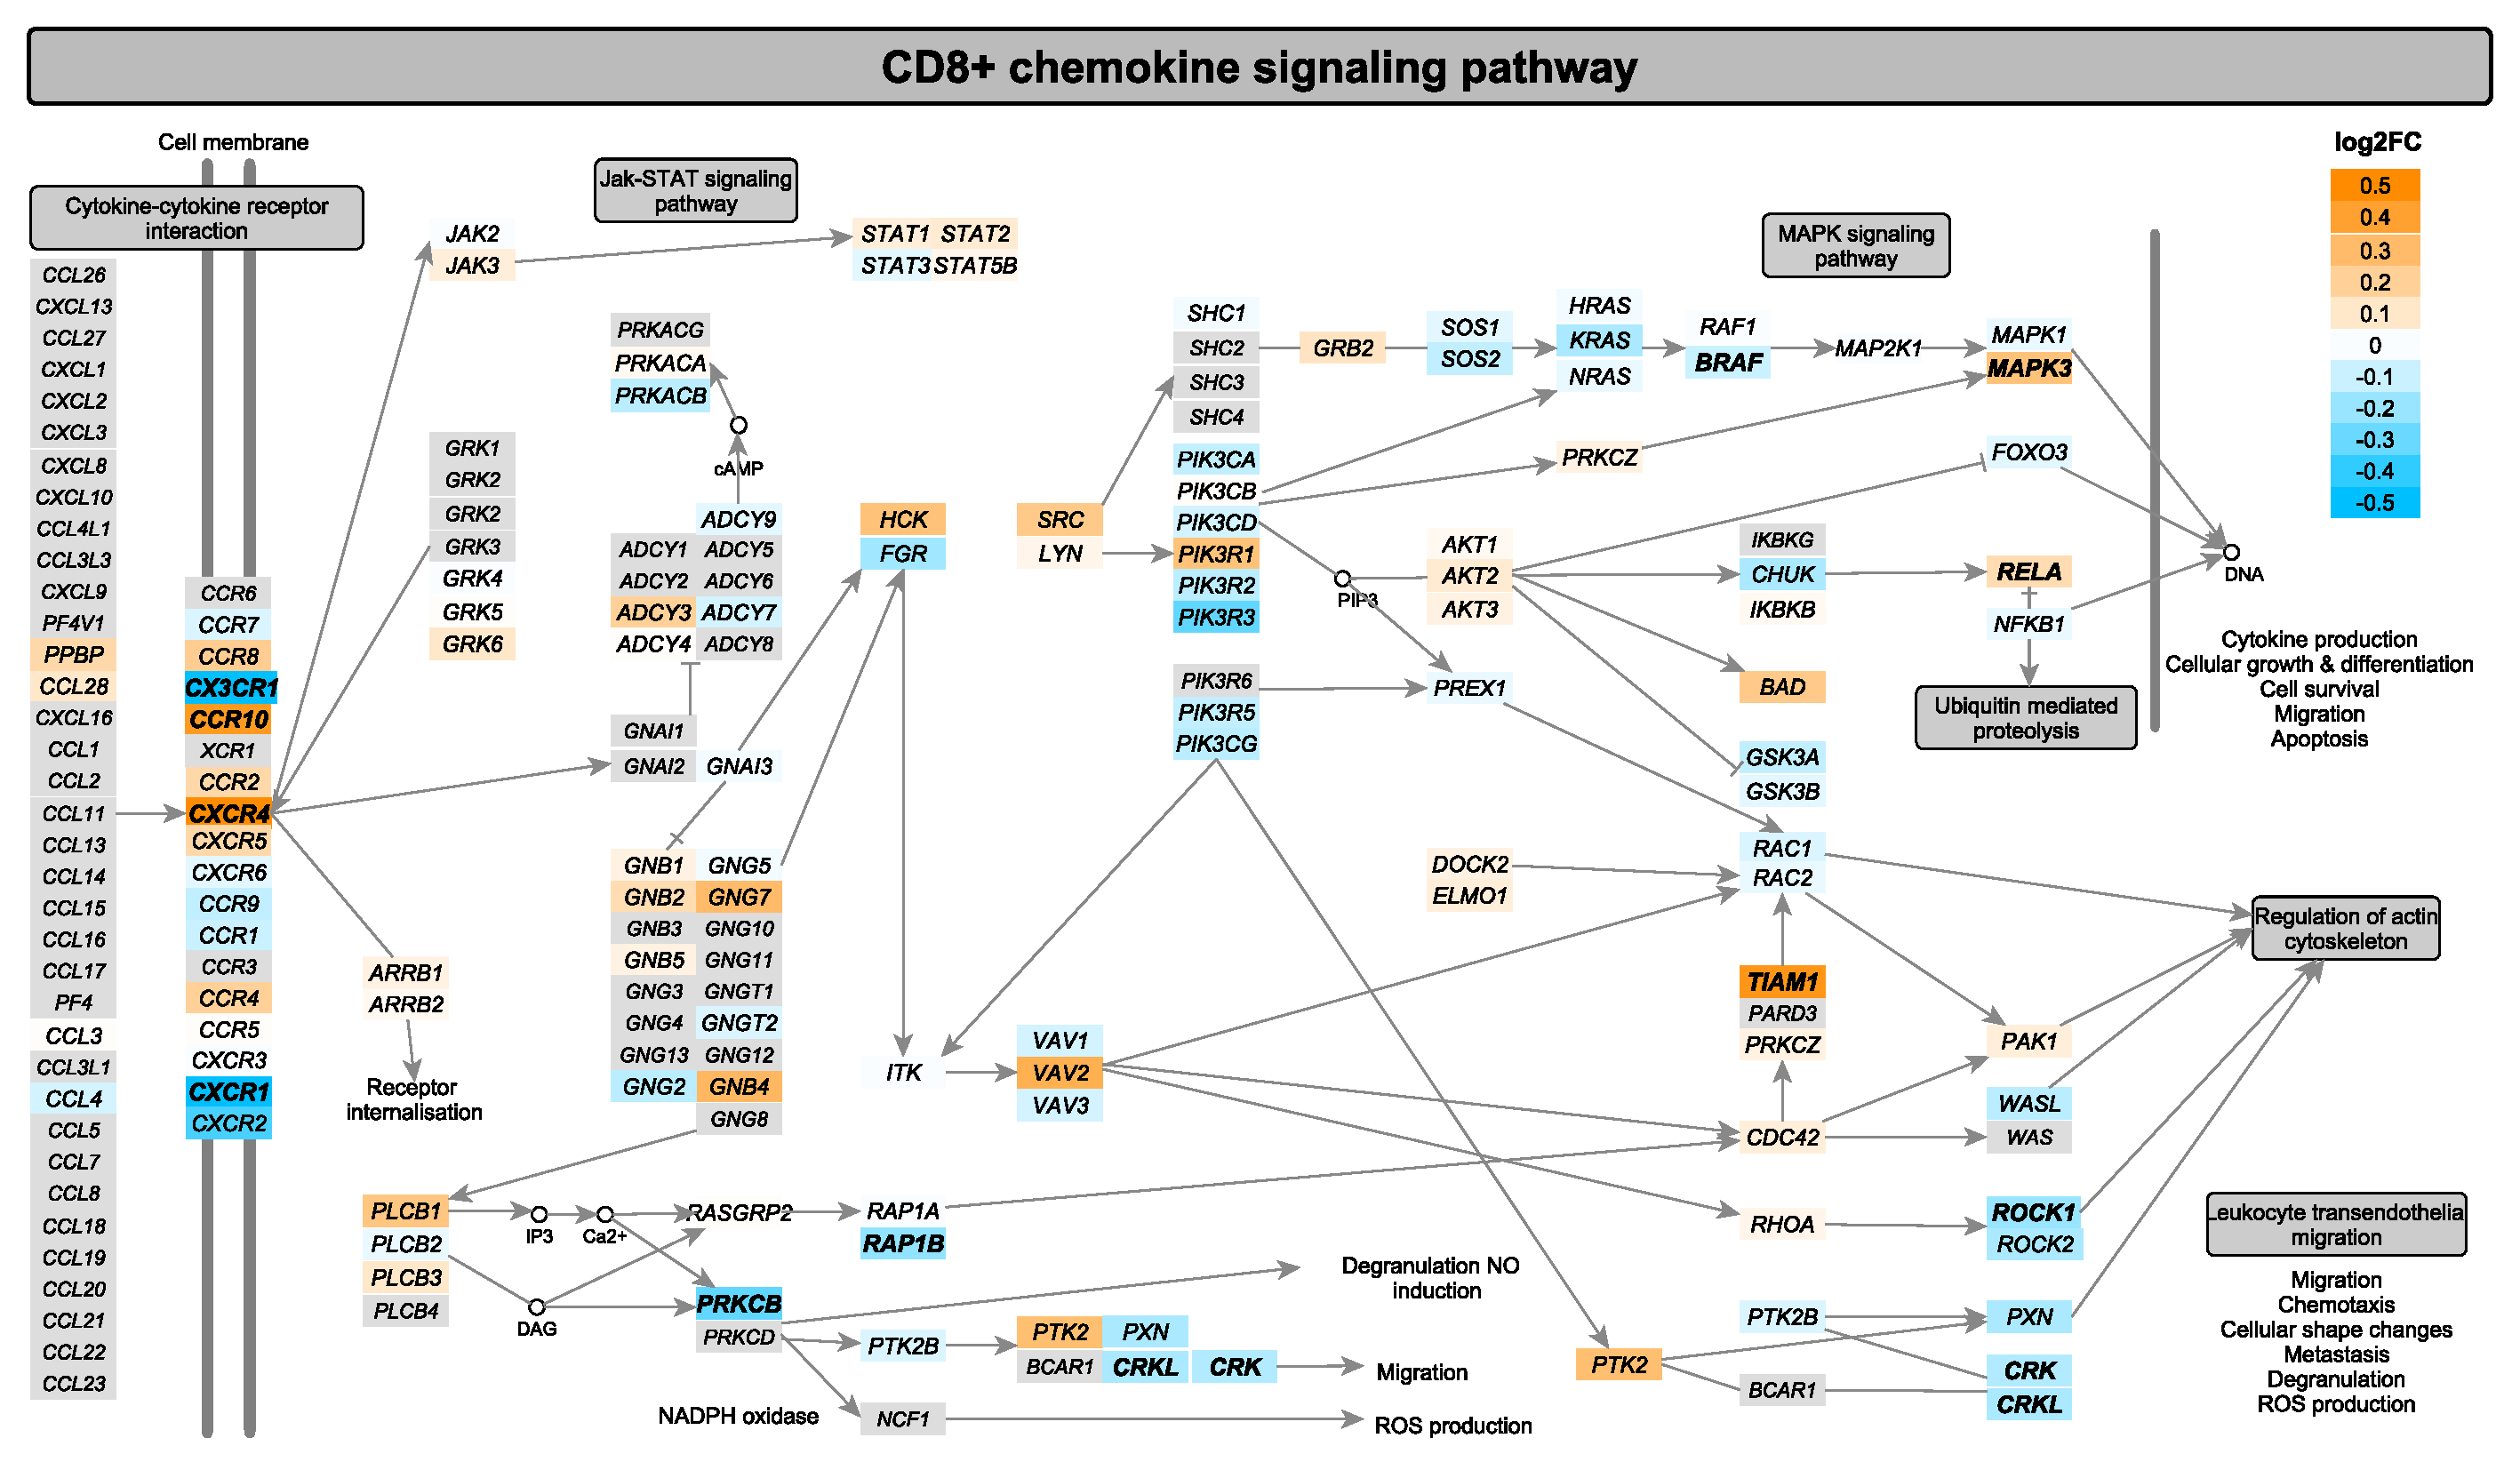
\includegraphics[width=\textwidth]{./Results2/pdfs/PS_CTL_CD8_all_chemokine_pathway}
\caption{\textbf{}}
\end{subfigure}
\caption[Mapping of the DEGs identified in CD8$^+$ cells between psoriasis patients and healthy controls onto the TNF-$\alpha$ and the chemokine signalling pathways.]{\textbf{Mapping of the DEGs identified in CD8$^+$ cells between psoriasis patients and healthy controls onto the TNF-$\alpha$ and the chemokine signalling pathways.} The a) TNF-$\alpha$ and b) chemokine pathways were sourced from KEGG, manually curated in a way that all member genes are maximised visually and then automatically color-coded by the log$_2$FC expression between psoriasis patients and healthy controls CD8$^+$ cells isolated from PB. Significant DEGs (FDR$<$0.05) are highlighted in bold. In a), members of the TNF-$\alpha$ pathway shared with the NF-$\kappa$B are highlighted with a green box. Additional members of the NF-$\kappa$B pathway differentially regulated in CD8$^+$ cells have also been indicated in brackets. Enrichment for a) and b) was identified by using only the CD8$^+$ DEGs (FDR$<$0.05).}
\label{figure:NAseq_PS_CTL_CD8_TNF_and_chemokine_pathway_modified}
\end{figure}





Other genes with a prominent pro-inflammatory role also appeared to be down-regulated in the NF-$\kappa$B or TNF signalling pathways, such as the activating transcription factor 2 (\textit{ATF2}) and 4 (textit{ATF4}) members of the TNF signalling cascade and the protein kinase C beta\textit{PRKCB} from the NF-$\kappa$B and chemokine signalling pathways. Notably, \textit{ATF4} was found to be up-regulated in CD noninflammed ileal biopsies causing activation of autophagy genes, whilst its expression was down-regulated in biopsies with active CD, pointing towards dysregulation of this pathway in disease onset \parencite{Bretin2016}. In contras, up-regulation of pro-inflammatory genes members of these two pathways were also found. For example JunB proto-oncogene (\textit{JUNB}) coding for one of the subunits of the TF AP-1 and three of the NF-$\kappa$B subunits including \textit{RELA}, \textit{RELB} and \textit{NFKB2}. Particularly, AP-1 undergoes activation following growth factors, cytokines, chemokines, hormones and multiple environmental stresses and acts as a negative regulator of cell proliferation and IL-6 production \parencite{Schonthaler2011} Although in psoriasis lesional skin AP-1 protein levels have been found to be down-regulated, JunB was found to be increased both, at the protein and mRNA levels, consistently with this observation in CD8$^+$ circulating cells \parencite{Johansen2004}.

Regarding dyregulation of chemokines, a mix of up-regulation and down-regulation of members of this pathway was found in CD8$^+$ cells from psoriasis patients when compared to healthy controls (Figure \ref{figure:RNAseq_PS_CTL_CD8_TNF_and_chemokine_pathway_modified} b) and no changes were found in CD4$^+$ cells. One of the most relevant dysregulated cytokine genes was \textit{CCR10}, the receptor for the chemotactic skin-associated chemokine CCL27. In this data CD8$^+$ cells from psoriasis patients presented up-regulated expression of the \textit{CCR10} receptor. Some studies have demonstrated an increased of CCR10$^+$ infiltrated T lymphocytes in psoriasis \parencite{Homey2002}. In circulation, expression of CCR10 is restricted to the a subset of circulating mCD4$^+$ and mCD8$^+$ T cells expressing the cutaneous lymphocyte-associated antigen (CLA), which are preferentially recruited to cutaneous sites of inflammation where KCs express CCL27 \parencite{Hudak2002}. A study in psoriasis circulating cells revealed a correlation between the frequency of CTLA$^+$ CD8$^+$ cells and disease severity measured by PASI score \parencite{Sigmundsd\'{o}ttir2001}. Other up-regulated chemokine receptors in CD$^+$ circulating psoriatic cells included \textit{CXCR4} gene (receptor for CXCL12) for which controversial finding have been reported about its role in skin inflammation and psoriasis \parencite{Zgraggen2014,Takekoshi2013}.

TNF:
% ATF4 https://www.tandfonline.com/doi/full/10.1080/15548627.2016.1156823
%JUNB up in psoriasis https://www.jidonline.org/article/S0022-202X(15)32827-X/fulltext;https://www.ncbi.nlm.nih.gov/pubmed/15377346
%PKCB https://www.ncbi.nlm.nih.gov/pmc/articles/PMC5594653/


\subsection{RNA-seq in epidermis from psoriasis patients}
\subsubsection{Quality control of the RNA-seq data}
For the three paired samples, both the uninvolved and the lesional samples presented a mapping rate greater than 80\% for all the samples, being the rate moderately greater in the lesional compaired to the uninvolved samples in all the three patients (Figure \ref{RNAseq_PS_uninvolved_lesional_psoriasis_skin_mapping_and_PCA} a). The number of reads after filtering non-uniquely mapped and duplicated reads that were mapped to Ensembl genes ranged between 29.5 and 33.2 million in PS1011 uninvolved and PS1011 lesional, respectively (Figure \ref{figure:RNAseq_PS_uninvolved_lesional_psoriasis_skin_mapping_and_PCA} b). Similarly to the mapping rate, the final million of reads mapping to genes after filtering was also greater in the lesional samples compared to the controls, not differing in more than 4 million reads.


\begin{figure}[htbp]
\centering
\begin{subfigure}{0.5\textwidth}
\centering
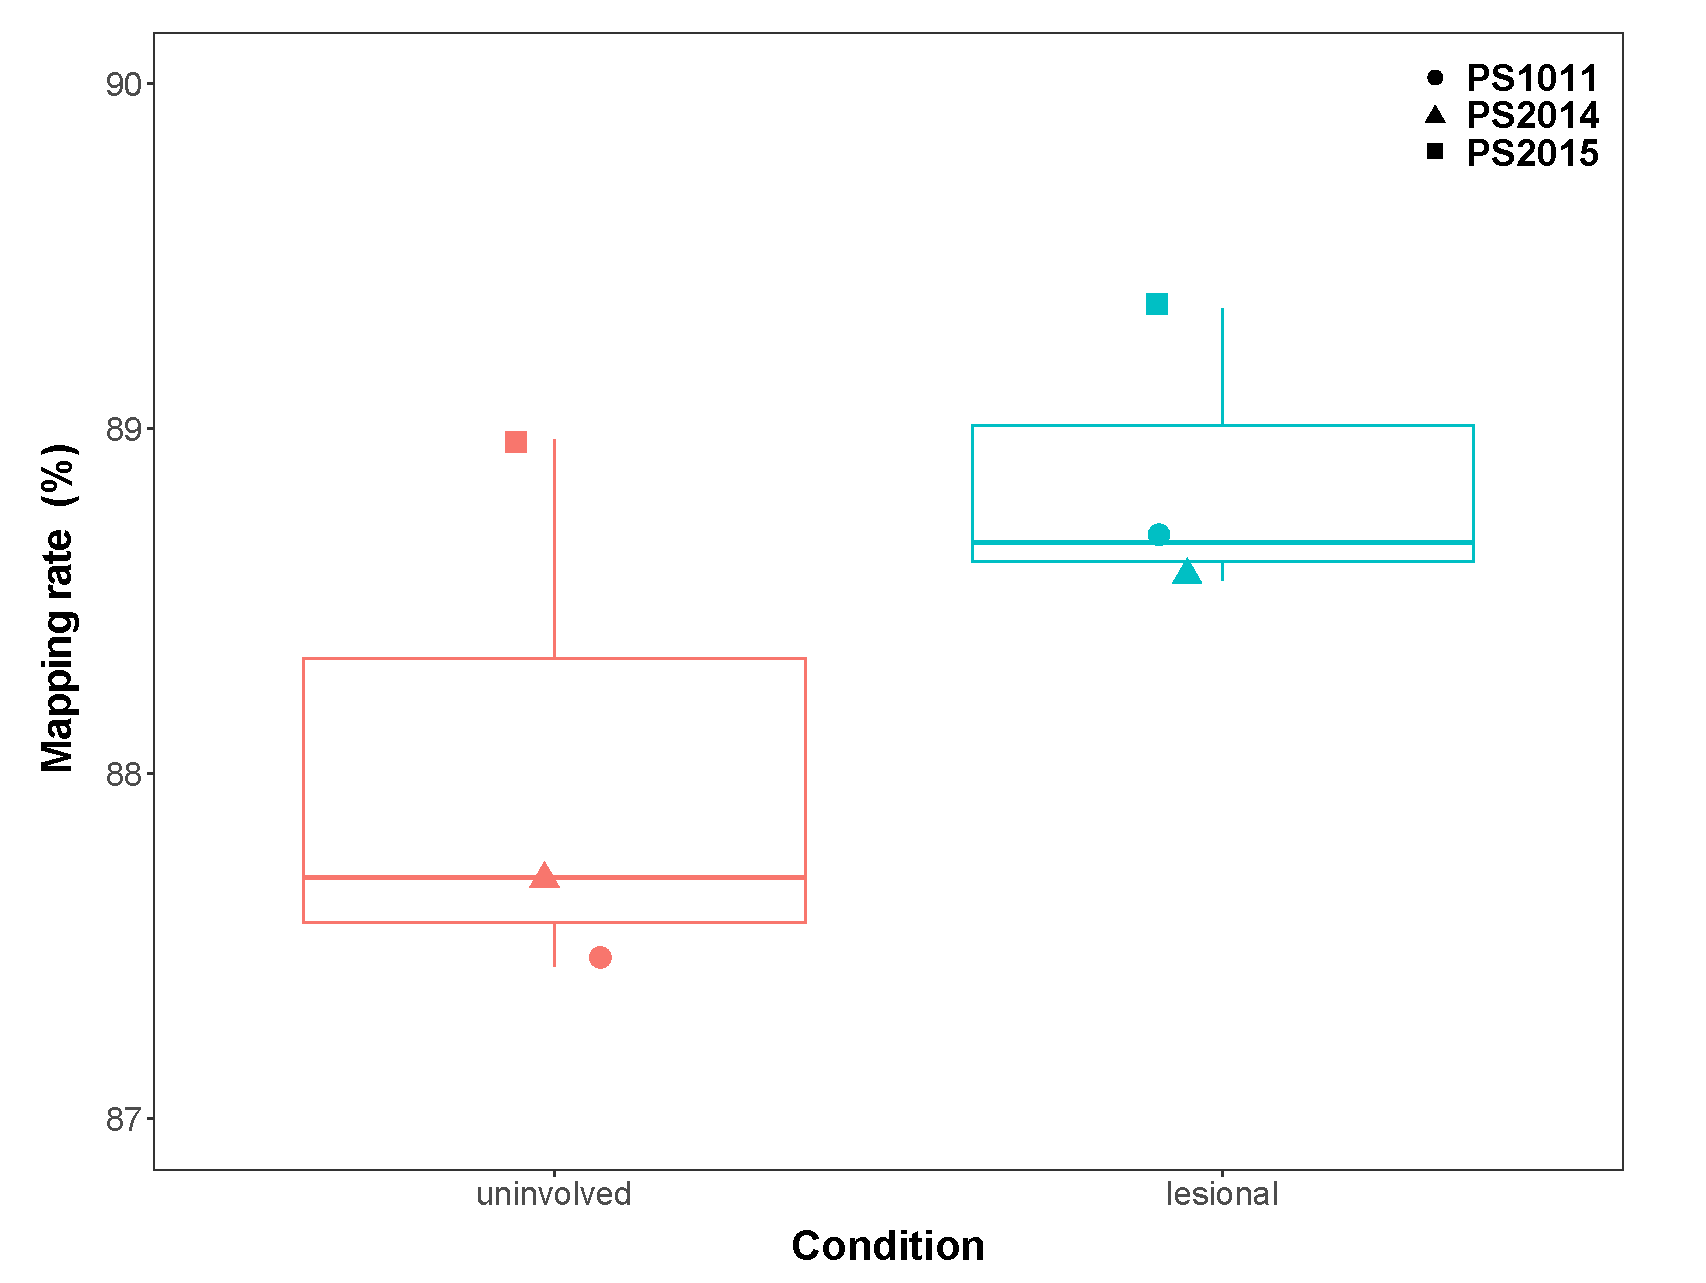
\includegraphics[width=\textwidth]{./Results2/pdfs/PS_lesional_uninvolved_RNAseq_uniquely_mapped_reads_percent_cell_type_and_batch_boxplots}
\caption{\textbf{}}
% The percentage sign indicated that the other subfig goes side by side
\end{subfigure}%
\begin{subfigure}{0.5\textwidth}
\centering
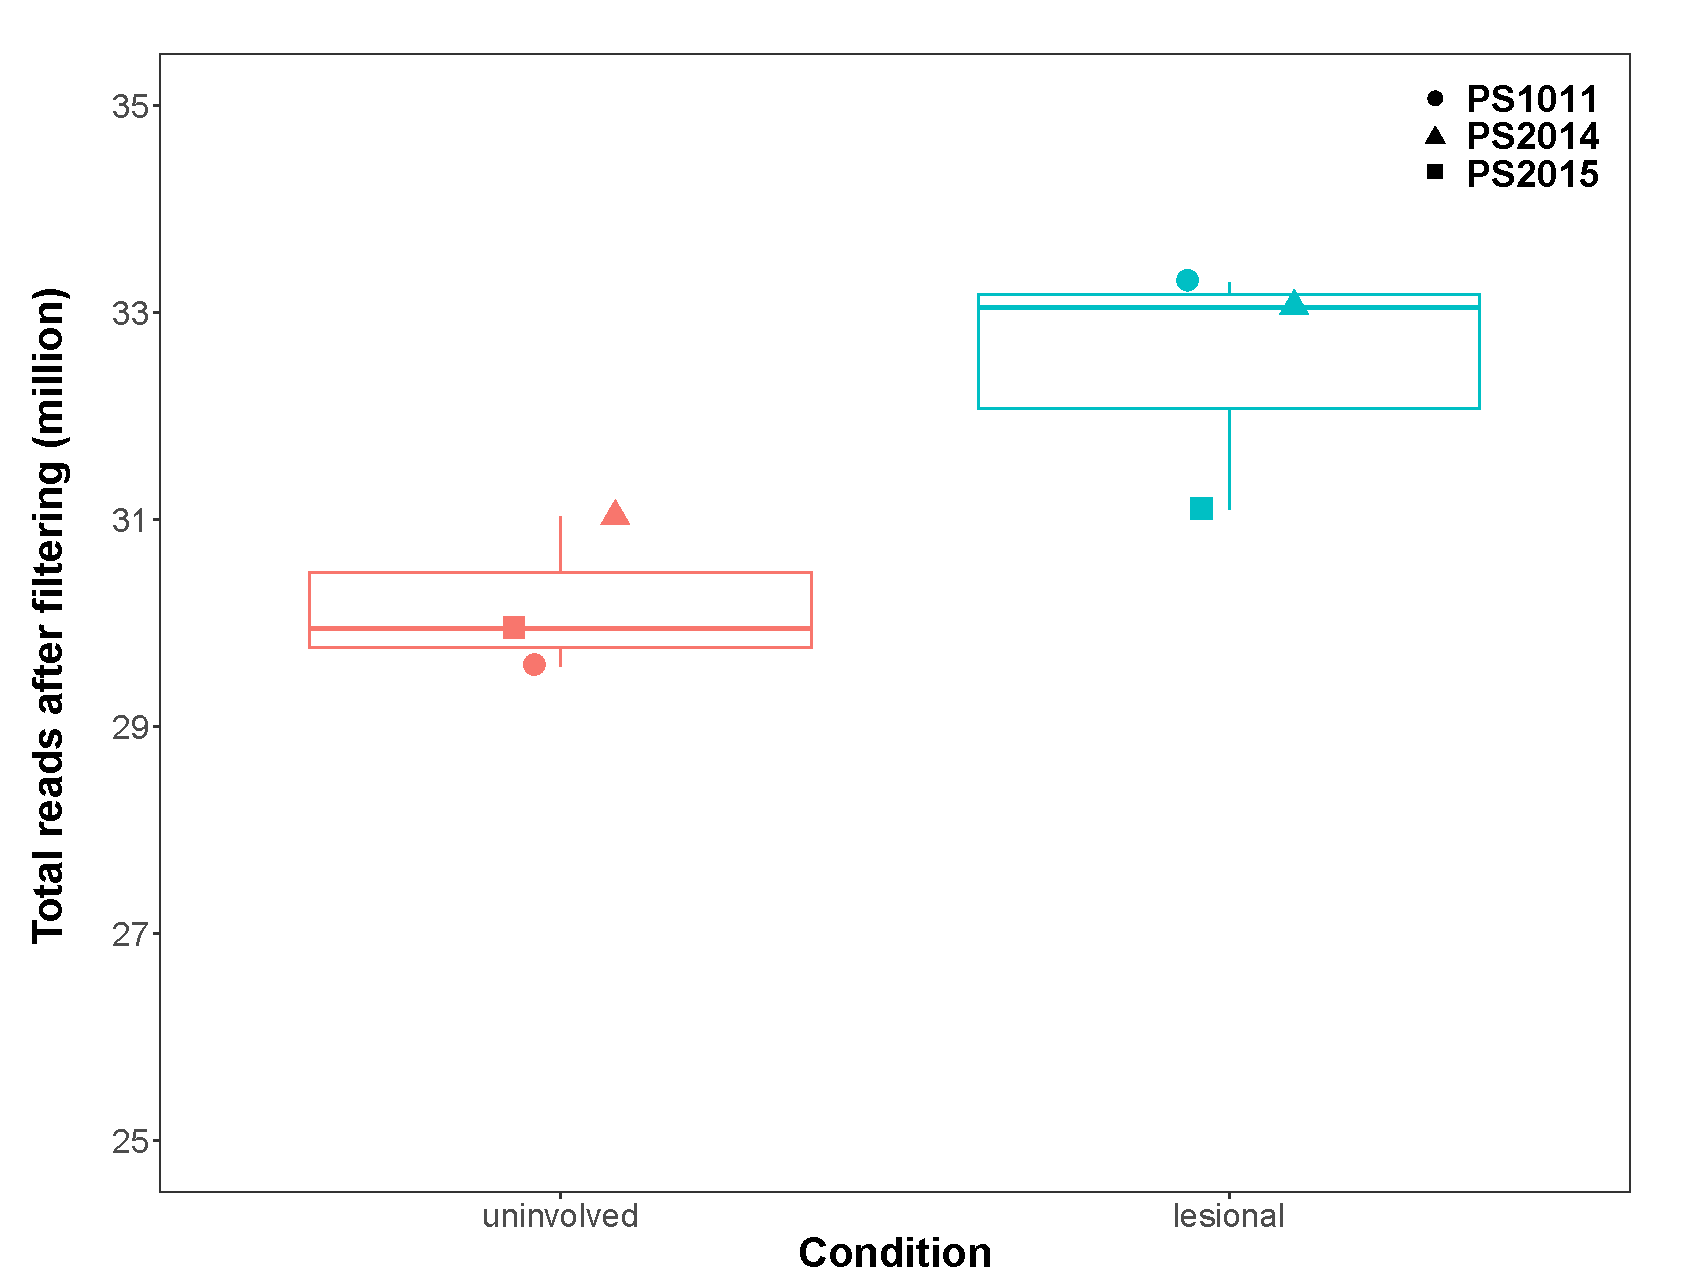
\includegraphics[width=\textwidth]{./Results2/pdfs/PS_lesional_uninvolved_RNAseq_total_reads_per_cell_type_and_batch}
\caption{\textbf{}}
\end{subfigure} \\
\begin{subfigure}{0.4\textwidth}
\centering
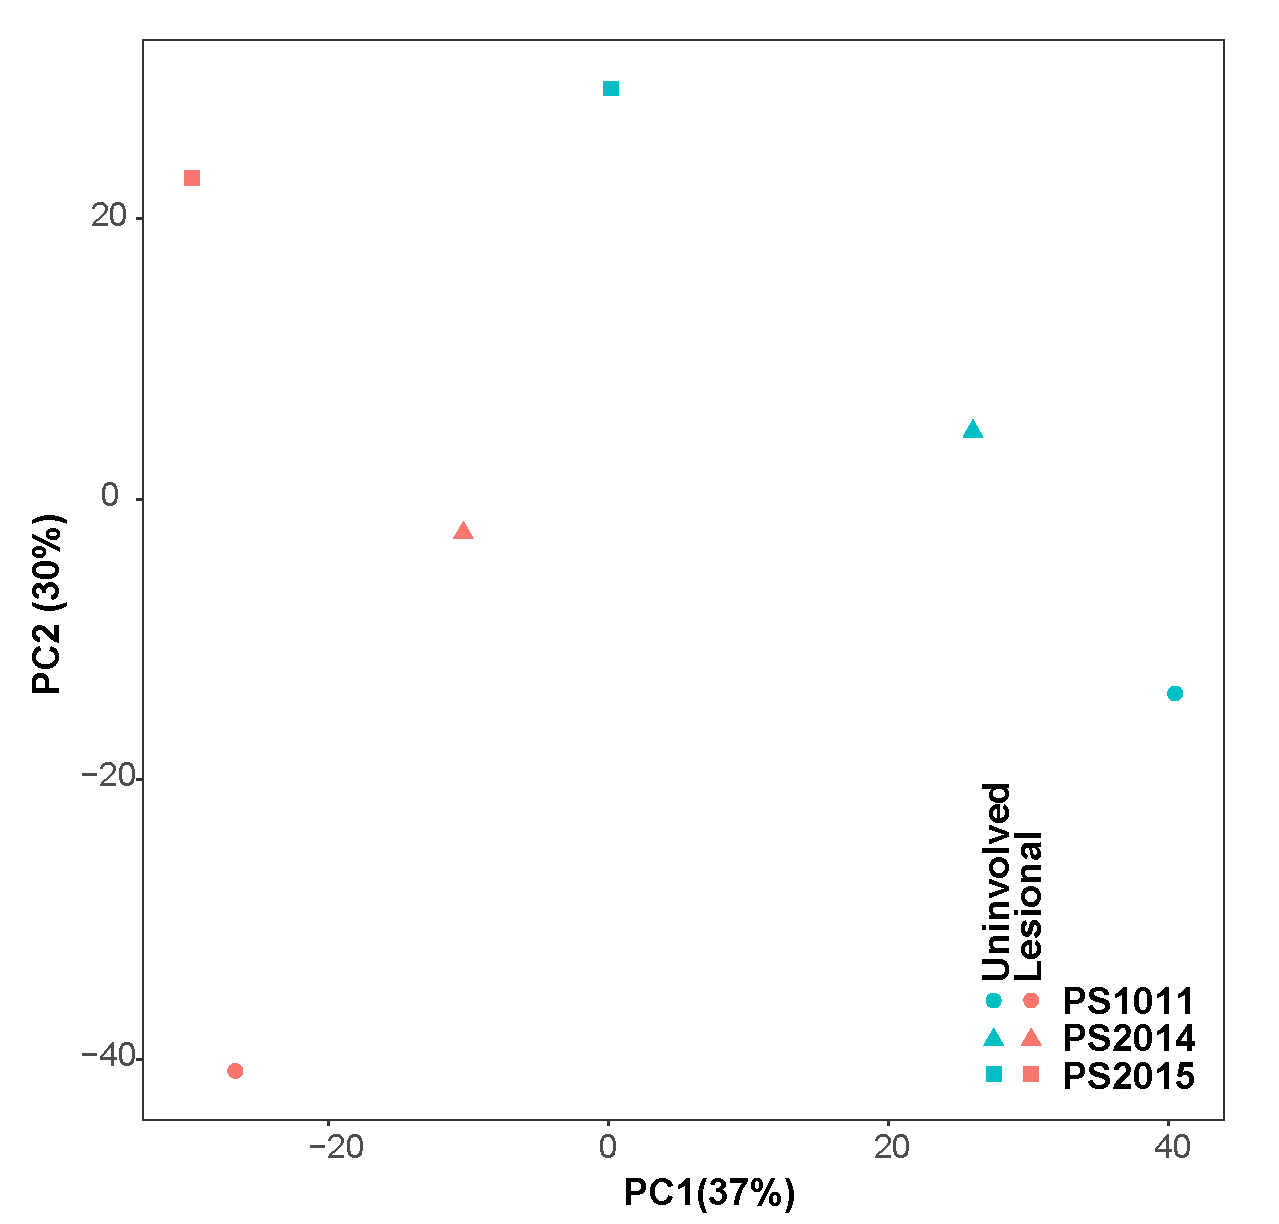
\includegraphics[width=\textwidth]{./Results2/pdfs/PS_lesional_uninvolved_varied_PCA1and2_plot}
\caption{\textbf{}} % to add text to the figure name
\end{subfigure}%
\caption[Mapping quality control and PCA analysis for the RNA-seq data in the uninvolved and lesional epidermis from psoriasis patients.]{\textbf{Mapping quality control and PCA analysis for the RNA-seq data in the uninvolved and lesional epidermis from psoriasis patients.} a) Mapping rate calculated as the proportion of sequencing reads mapping uniquely to a particular region of the genome. b) The total number of reads mapping to an Ensembl feature (including protein coding genes and lncRNAs) after removing the non-uniquely mapped and duplicated reads. c) First and second component of the PCA analysis performed on the normalised number of reads mapping to the Ensmbl list of mRNAs and lncRNAs.}
\label{figure:RNAseq_PS_uninvolved_lesional_psoriasis_skin_mapping_and_PCA}
\end{figure} 

PCA analysis using the normalised number of reads mapping to the genes after filtering (see Chapter \ref{ch:Mat}) revealed separation the lesional samples from the uninvolved by the first PC, which explained 37\% of the variance (Figure \ref{figure:RNAseq_PS_CTL_uninvolved_lesional_psoriasis_skin_mapping_and_PCA} c). The second PC explained 30\% of the variance and correlated with the patients ID. Overall, PCA analysis revealed substantial variation between the lesional and uninvolved samples and also showed biological variability between individuals, for which the paired design in the DGE analysis was accounting for.  


\subsubsection{Summary of the DGE results}

DGE analysis  revealed a total of 1,227 (FDR$<$0.05) and 702 (FDR$<$0.01) genes dysregulated between the uninvolved and lesional epidermis skin biopsies, including mRNAs and lncRNAs (Table \ref{RNAseq_PS_lesional_uninvolved_DGE_results}). Amongst the 1,227 DEGs, a similar proportion of genes up- (559 genes) and down-regulated (629) in lesional skin when compared to uninvolved were identified (vulcano plot). Moreover, the FCs in gene expression were notably larger when compared to the changes in expression from analysis in circulating immune cells.  

\begin{table}[htbp]
%\setlength{\tabcolsep}{20pt} only to stretch the columns if you want
%\renewcommand{\arraystretch}{1.5}
\centering
\begin{tabular}{@{} c c c c}
\toprule
\textbf{FDR threshold}   & \textbf{mRNA}   & \textbf{lncRNA}  & \textbf{Overlap with}\\
                         &                 &                  & \textbf{GWAS genes}\\
\midrule
\midrule
0.05                     & 1181            & 46               &  up(\textit{IFIH1}, \textit{NOS2}, \textit{STAT3},\\ 
                         &                 &                  &  \textit{LCE3D}), down(\textit{TNFAIP3}) \\
0.01                     &  677            & 25               &  \textit{NOS2}, \textit{STAT3},\textit{TNFAIP3},\textit{LCE3D} \\
\bottomrule 
\end{tabular}
\medskip %gap
\caption[Summary results of the DGE analysis between uninvolved and lesional psoriatic epidermal biopsies.]{\textbf{Summary results of the DGE analysis between uninvolved and lesional psoriatic epidermal biopsies.} Number of differentially expressed mRNAs and lncRNAs are reported for two threshold of significance (FDR$<$0.05 and FDR$<$0.01). The DEGs overlapping putative psoriasis GWAS genes and the directionality in the change of expression are also specified.}
\label{tab:RNAseq_PS_lesional_uninvolved_DGE_results}
\end{table}
\bigskip %bigger spac


Amongst the DEGs between the uninvolved and lesional skin in our study, four genes (FDR$<$0.05) overlapped with putative GWAS genes (Table \ref{RNAseq_PS_lesional_uninvolved_DGE_results}). \textit{IFIH1}, \textit{NOS2}, \textit{LCE3D} and \textit{STAT3} were also found to be up-regulated in lesional compared to uninvolved skin biopsies from psoriasis patients in \parencite{Tsoi2015}. In contrast, \textit{TFNAIP3} was found to be up-regulated in \parencite{Jabbari2011}, opposite to our finding.


\subsubsection{Overall comparison with other skin transcriptomic studies}

As previously mentioned, the approach to perform the study of DGE in skin is different from most of the previously published studies using whole punch biopsies to compare lesional and uninvolved skin from psoriasis patients. During the course of this project a study published by Tervaniemi and colleagues also aimed to characterise the transcriptional profiles of the epidermis from psoriasis patients lesional and uninvolved skin in a more elegant way than the previous studies using whole skin thickness biopsies.  As previously detailed, Tevaniemi \textit{et al.}, 2016 had a bigger sample size (six psoriasis patients) compared to this study (three psoriasis patients) and also included nine controls epidermis biopsies. In order to explore the similarities between the two studies, a comparison for the DEGs identified in both studies was conducted. Tervaniemi reported a total of 2,589 DEGs passing their filtering criteria (FC$<$0.75 or FC$>$1.5 and FDR$<$0.05). In contrast to our findings, the number of genes up-regulated in lesional epidermis compared to uninvolved (2,330) was larger than the number of down-regulated targets (261). Regarding overlap, a total of 359 out of the 1,227 DEGs (29.25\%) identified in our study were shared with Tervaniemi results, of which 239 and 75 were up- and down-regulated, respectively. The direction of change in 45 out of the 359 shared genes appeared to be opposite across the two datasets. An example is the \textit{SERPINB2} gene, a serine protease inhibitor of the serpin superfamily which presented down-regulation in our data and cultured lesional KCs from Swindell \textit{et al.}, 2017 in contrast to the up-regulation in Tervaniemy results. Interestingly, an study demonstrated a defective stratum corneum in \textit{SERPINB2} deficient mice as well as greater susceptibility to developing inflammatory lesions upon chemically induced atopic dermatitis compared to wild type controls \parencite{Schroder2016}.   


In addition to Tervaniemi study, our results were further contrasted to one of the most recent comprehensive RNA-seq study comparing lesional and uninvolved full thickness skin biopsies from psoriasis patients \parencite{Tsoi2015}. Out of the 3,723 DEGs reported by Tsoi and colleagues, 507 genes were shared between the two studies (41\% of the genes from this project), of which 272 were up-regulated and 228 appeared to be down-regulated. Interestingly, despite the larger sample size, the DEGs between lesional and uninvolved skin from the Tsoi and colleagues study did not capture all the dyregulated genes from our study. This could suggest that our approach using more KCs enriched sample may be more sensitive to detect changes of gene expression that are masked when using whole punch biopsies. Amongst the 507 genes, only 7 (\textit{ALOX15B},  \textit{ARG2}, \textit{LCE6A},\textit{MGST1}, \textit{PNLIPRP3}, \textit{TLDC1} and \textit{UBL3}) presented opposite direction of change in the two studies. Amongst the genes showing opposite directions was \textit{LCE6A}, one of the \textit{LCE} gene family involved in the synthesis of the later cornified envelope layer, was down-regulated in lesional skin in our study, in contrast to the up-regulation found in the Tsoi analysis. Similarly, in the previous comparison, other genes from the LCE family, including \textit{LCE1B}, \textit{LCE1F} and \textit{LCE2A} appeared also down-regulated in our data and up-in the Tervaniemi study. In contrast to discrepancies in other \textit{LCE} genes, all three datasets presented up-regulation of the GWAS risk associated gene \textit{LCE3B}. Notably, qPCR quantification of \textit{LCE} genes from groups 1, 2, 5 and 6 demonstrated increased expression in psoriasis lesional skin \parencite{Bergboer2011}. 


Overall, the comparison of our results with these two studies suggested greater similarities with the full skin thickness biopsies from Tsoi \textit{et al.}, 2015 in terms DEGs overlapping due to different technical reasons, as further detailed in the Discussion. 


\subsubsection{Dysregulated lncRNAs in the psoriatic lesional skin}

In addition to protein coding genes, a total of 46 lncRNAs were also significantly (FDR$<$0.05) differentially expressed between uninvolved and lesional skin from the three psoriasis patients. Similarly to the results presented for the circulating immune cells, the vast majority of  modulated lncRNAs were functionally uncharacterised difficulting the interpretation of this results. 24 out of the 46 dysregulated lncRNAs were also reported as differentially expressed by Tsoi and colleagues. An interesting  example is \textit{H19} which was significantly down-regulated in the lesional skin when compared to uninvolved. H19 has been described to directly bind miR-130b-3p which down-regulates Desmoglein 1 (\textit{DSG1}), a gene promoting KCs differentiation \parencite{Li2017}. This finding was consistent with Tsoi \textit{et al.}, 2015 and also with results from Li \textit{et al.}, 2014 and \textit{et al.}, 2016 where they compared lesional versus normal skin. 

Interestingly, four miRNAs (\textit{MIR146A}, \textit{MIR22HG}, \textit{MIR31HG} and \textit{MIR205HG}) were also captured with the standard library preparation for mRNAs and lncRNAs implemented in our project. The relevance of miR-146A has been already commented in the DGE analysis from circulating immune cells. In lesional skin \textit{MIR146A} was up-regulated when compared to uninvolved skin, consistently with other studies \parencite{Lerman2014, Tsoi2015}, and also shown increase its expression when comparing lesional skin versus healthy biopsies \parencite{Li2014}. Moreover, a polymorphisms in miR-146a has been associated with psoriasis in a small cohort study and a \textit{MIR146A} knock-out mice with chemical induced psoriasis led to earlier disease onset and amplified epidermal activation \parencite{Srivastava2017}. Another relevant finding was the up-regulation of \textit{MIR31HG} in lesional skin, which has also been reported by \parencite{Tsoi2015}. Notably, a functional study using the KCs immortal cell line HaCaT demonstrated that silencing miR-31hg induces cell cycle arrest and inhibits cell proliferation consistently with two characteristic functions dysregulated in psoriatic KCs \parencite{Gao2018}.

%\begin{table}[htbp]
%%\setlength{\tabcolsep}{20pt} only to stretch the columns if you want
%%\renewcommand{\arraystretch}{1.5}
%\centering
%\begin{tabular}{@{} c c c}
%\toprule
%\textbf{Transcript class}   & \textbf{Gupta \textit{et al.},}   & \textbf{Li \textit{et al.}}  \\
                            %& \textbf{2016}                     &      \textit{2014}            \\
%\midrule
%\midrule
%mRNA                        & xxx                               & xxxx                \\
%lncRNAs (functionally       & 2 (\textit{H19} (d),              & 7 (\textit{H19} (d), \textit{NEFL} (d), \textit{SCARNA2} (d),\\
%characterised)              & \textit{LINC00302} (u))           & \textit{SCARNA9} (d), \textit{SCARNA10} (d),\textit{UHRF1} (u),\\
                            %&                                   &  \textit{KCNQ1OT1} (d)) \\
%\bottomrule 
%\end{tabular}
%\medskip %gap
%\caption[Summary results of the DGE analysis between uninvolved and lesional psoriatic epidermal biopsies.]{\textbf{}u=up-regulated; d=down-regulated. Directionality for the differentially expressed lncRNA included in this table was concordant with other studies having reported them previously for all of them but \textit{LINC00302} which appeared down-regulated in this data.}
%\label{tab:RNAseq_PS_lesional_uninvolved_overlap_with_other_studies}
%\end{table}
%\bigskip %bigger spac



\subsubsection{Pathways enriched for the DEGs}

In order to better understand the functional role of the DEGs (FDR$<$0.05) between lesional and uninvolved epidermis from psoriasis patients skin biopsies, pathways enrichment analysis was performed. A considerable number of pathways were significantly enriched (FDR$<$0.005) for DEGs found in our analysis (Table \ref{RNAseq_PS_lesional_uninvolved_pathway_enrichment} and \ref{tab:RNAseq_PS_lesional_uninvolved_additional_pathways}). 


\begin{table}[htbp]
%\setlength{\tabcolsep}{20pt} only to stretch the columns if you want
%\renewcommand{\arraystretch}{1.5}
\centering
\begin{tabular}{@{}c}
\toprule
\textbf{Lesional versus uninvolved epidermis enriched pathways} \\
\midrule
\midrule
IFN-$\alpha$/$\beta$/signalling \\
Peroxisome proliferator-activated receptors (PPAR) signalling \\
NOD-like receptor signaling pathway \\
IL-17 signalling \\
IL2-mediated signalling \\
G protein coupled receptor (GPCR) ligand binding \\
Hypoxia-inducible factor 1 (HIF-1) signalling \\
Cytokine signalling in immune system \\
Cell cycle \\
Apoptosis \\
Arginine and proline metabolism \\
\bottomrule
\end{tabular}
\medskip %gap
\caption[Most relevant pathways enriched for DEGs between lesional and uninvolved epidermis isolated from psoriasis patients skin biopsies.]{\textbf{Most relevant pathways enriched for DEGs between lesional and uninvolved epidermis isolated from psoriasis patients skin biopsies.} Significant pathways for FDR$<$0.005. The analysis was performed using significantly DEGs FDR$<$0.05 and no FC threshold. Enriched pathways had a minimum of ten members overlapping with DEGs.}
\label{tab:RNAseq_PS_lesional_uninvolved_pathway_enrichment}
\end{table}


A number of pathways were related to alterations in cell cycle and metabolic processes, including hypoxia-inducible factor 1 (HIF-1) signalling, arginine and proline metabolism,glycolysis/gluconeogenesis and metabolism of amino acids and derivatives, amongst others. Dysregulation of similar functions have previously also been reported in other studies comparing lesional and uninvolved skin and genome-wide pathway analysis\parencite{Coda2012, Aterido2016, Tervaniemi2016}. HIF-I signalling has been found to be up-regulated in psoriasis skin likely through hypoxia caused by increased cell proliferation rates and epidermal thickening. Our data revealed up-regulation of \textit{HIF1A}, \textit{VEGFA}, \textit{ENO1} and \textit{NOS2}, amongst others (Figure \ref{figure:PS_lesional_vs_uninvolved_HIF_pathway}). Up-regulated expression of the hypoxia-inducible TFs HIF-1$\alpha$ and HIF-2$\alpha$ has been found in lesional skin and co-related with the increase in \textit{VEGF} transcript levels, a target gene regulated by HIFs that mediates the pathological angiogenesis driving psoriasis \parencite{Rosenberg2007}. 

\begin{figure}[htbp]
\centering
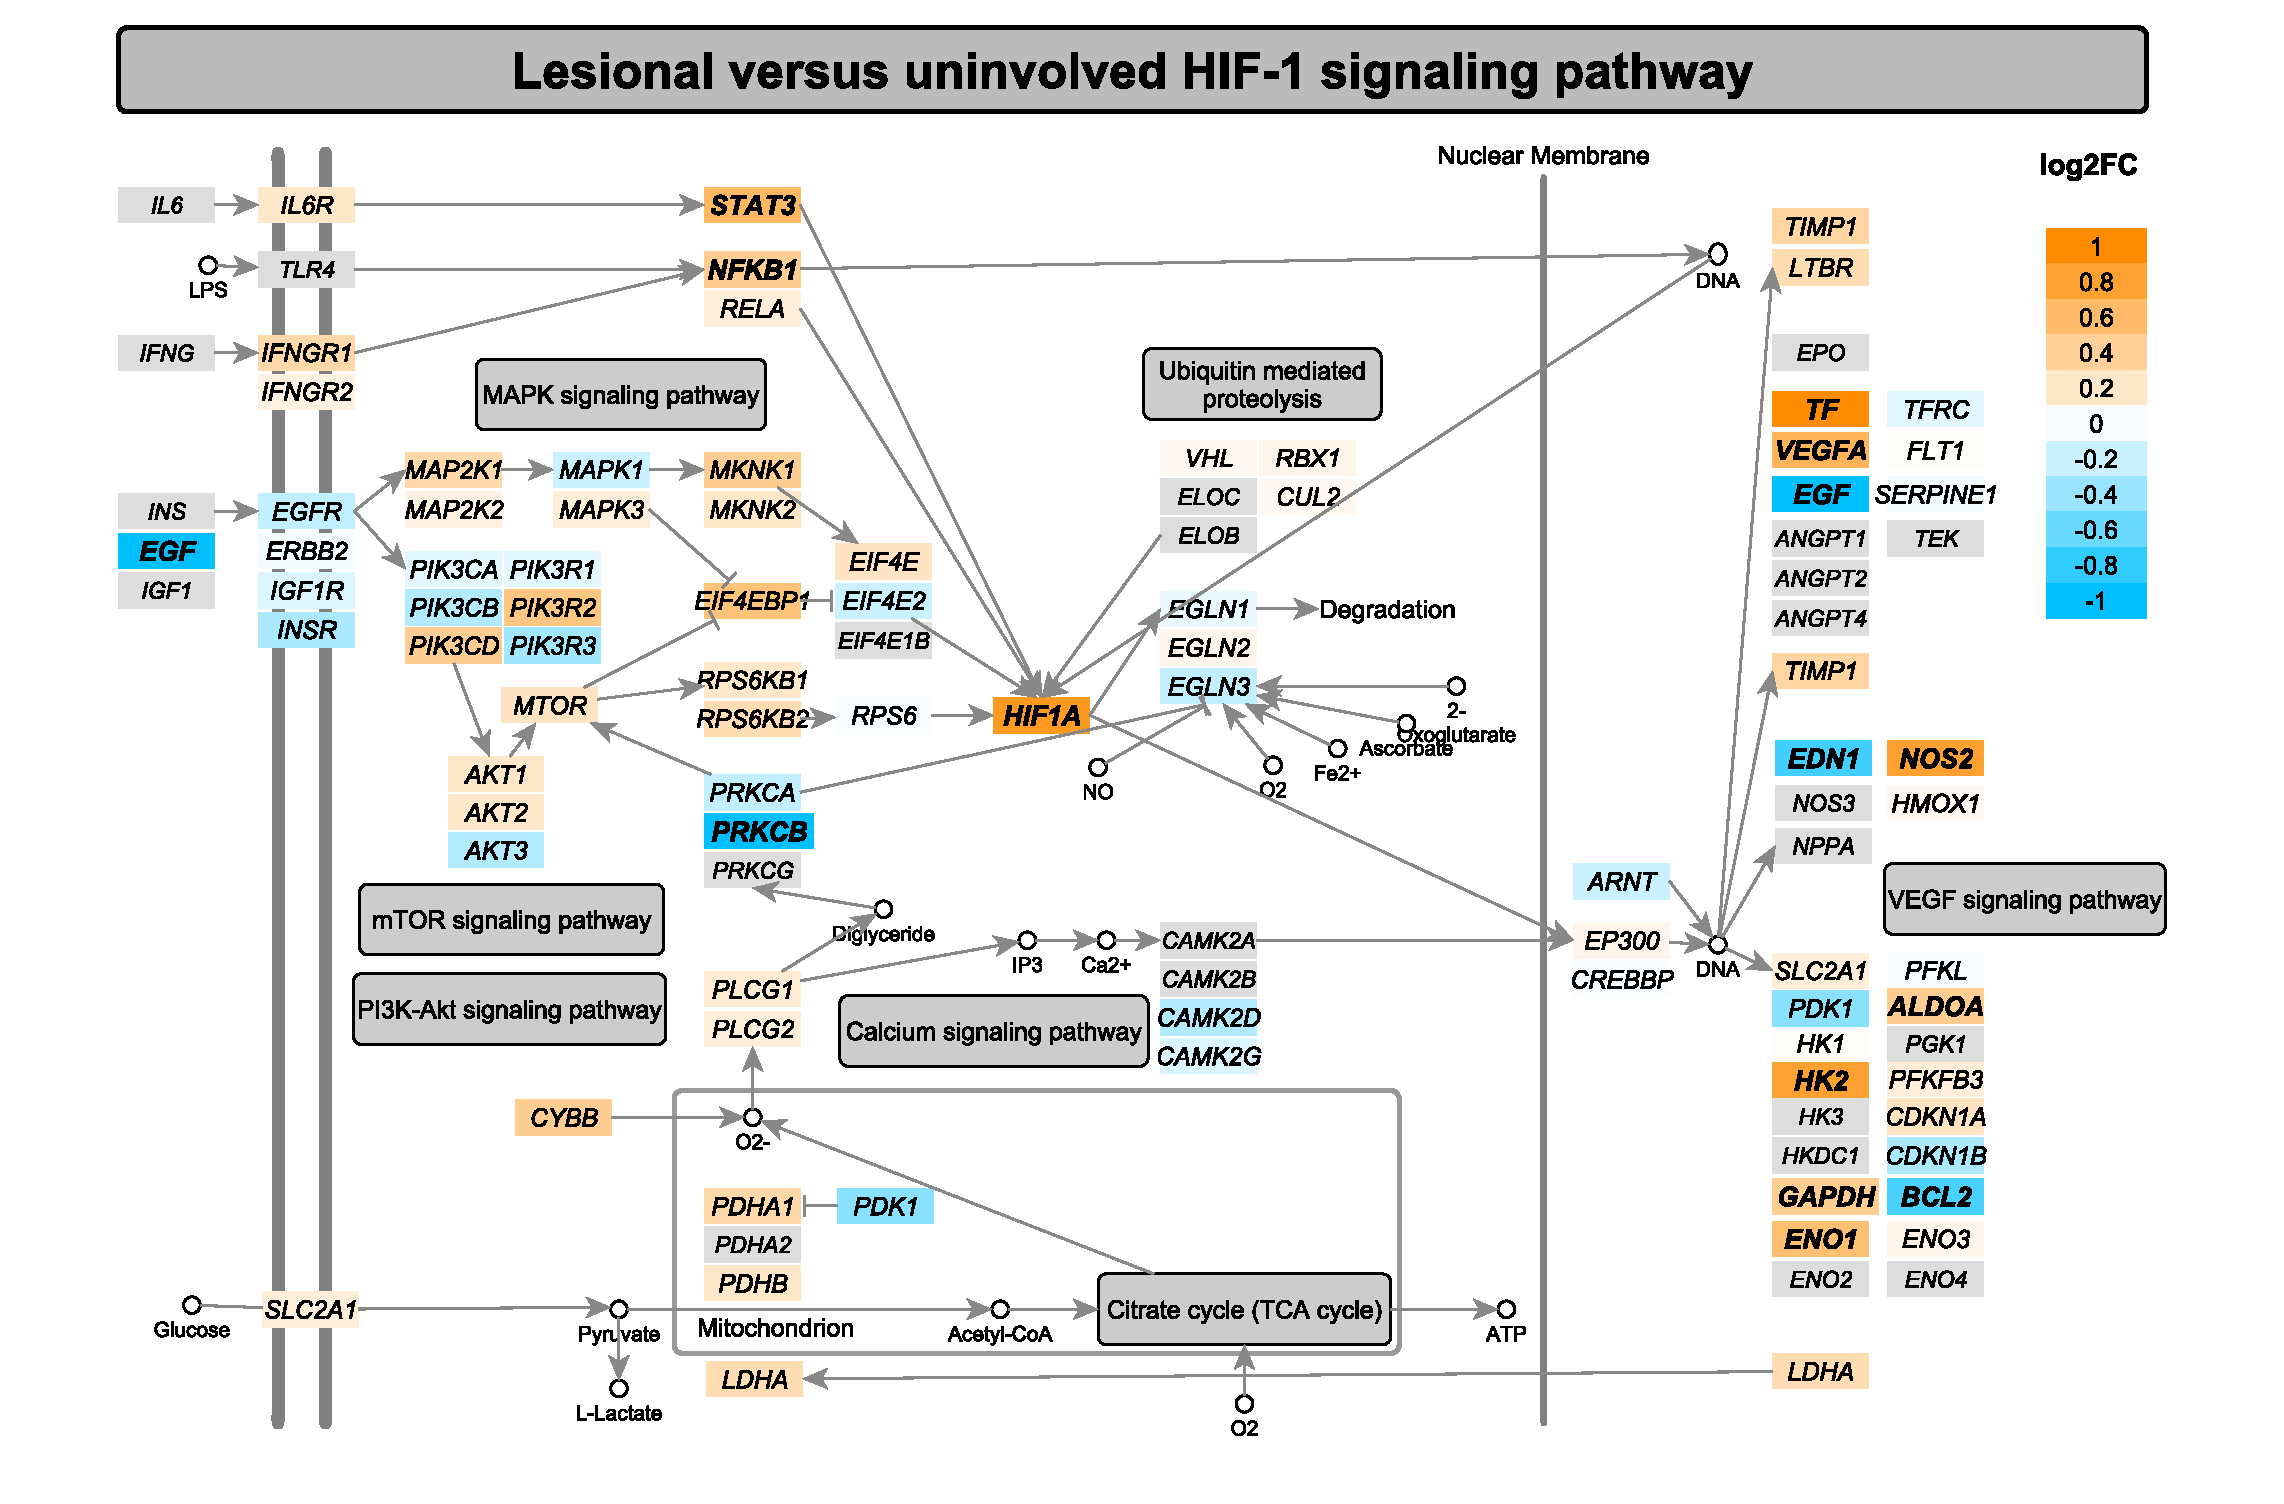
\includegraphics[width=0.9\textwidth]{./Results2/pdfs/PS_lesional_uninvolved_all_HIF_1_pathway}
\caption[Mapping of the DEGs between lesional and uninvolved epidermis from psoriasis patients onto the HIF-I signalling pathway.]{\textbf{Mapping of the DEGs between lesional and uninvolved epidermis from psoriasis patients onto the HIF-I signalling pathway.} This pathway was sourced from KEGG, manually curated in a way that all member genes are maximised visually and then automatically color-coded by the log$_2$FC expression between the lesional and uninvolved epidermis. Significant DEGs (FDR$<$0.05) are highlighted in bold. This pathway was identified by pathway enrichment analysis using only DEGs (FDR$<$0.05).}
\label{figure:PS_lesional_vs_uninvolved_HIF_pathway}
\end{figure}

Immune relevant pathways including IFN, IL-17 and NOD-like receptor signalling were also identified in this analysis. The NOD-like receptor pathway responsible for detecting various pathogens and generating innate immune responses through NF-$\kappa$B and MAPK activation, appeared enriched for 23 significantly DEGs (Figure \ref{figure:PS_lesional_vs_uninvolved_HIF_pathway} genes in bold). This pathway has also been identified as one of the most significantly enriched ones for DEGs in the epidermal study of Tervaniemi and colleagues. Some of the most up-regulated genes contributing to the enrichment included \textit{NOD2}, \textit{CARD6} or \textit{IFI16}, amongst others, and they were also up-regulated in Tervaniemi's data. Interestingly, pathway enrichment analysis using the DEGs from Tsoi and colleagues failed to show significant enrichment for NOD-I signalling. Nevertheless, NOD-I signalling remained significantly enriched (10 DEGs mapping to this pathway) when using for the analysis only the DEGs from our study not overlapping the Tsoi and colleagues ones. These results reinforced the failure of whole skin biopsies transcriptomics to identify additional NOD-I signalling genes differentially regulated between lesional and uninvolved skin and the value of studying epidermal biopsies to unveil exacerbated dysregulation of functional pathways in KCs.


\begin{landscape}
\begin{figure}[H]
\centering
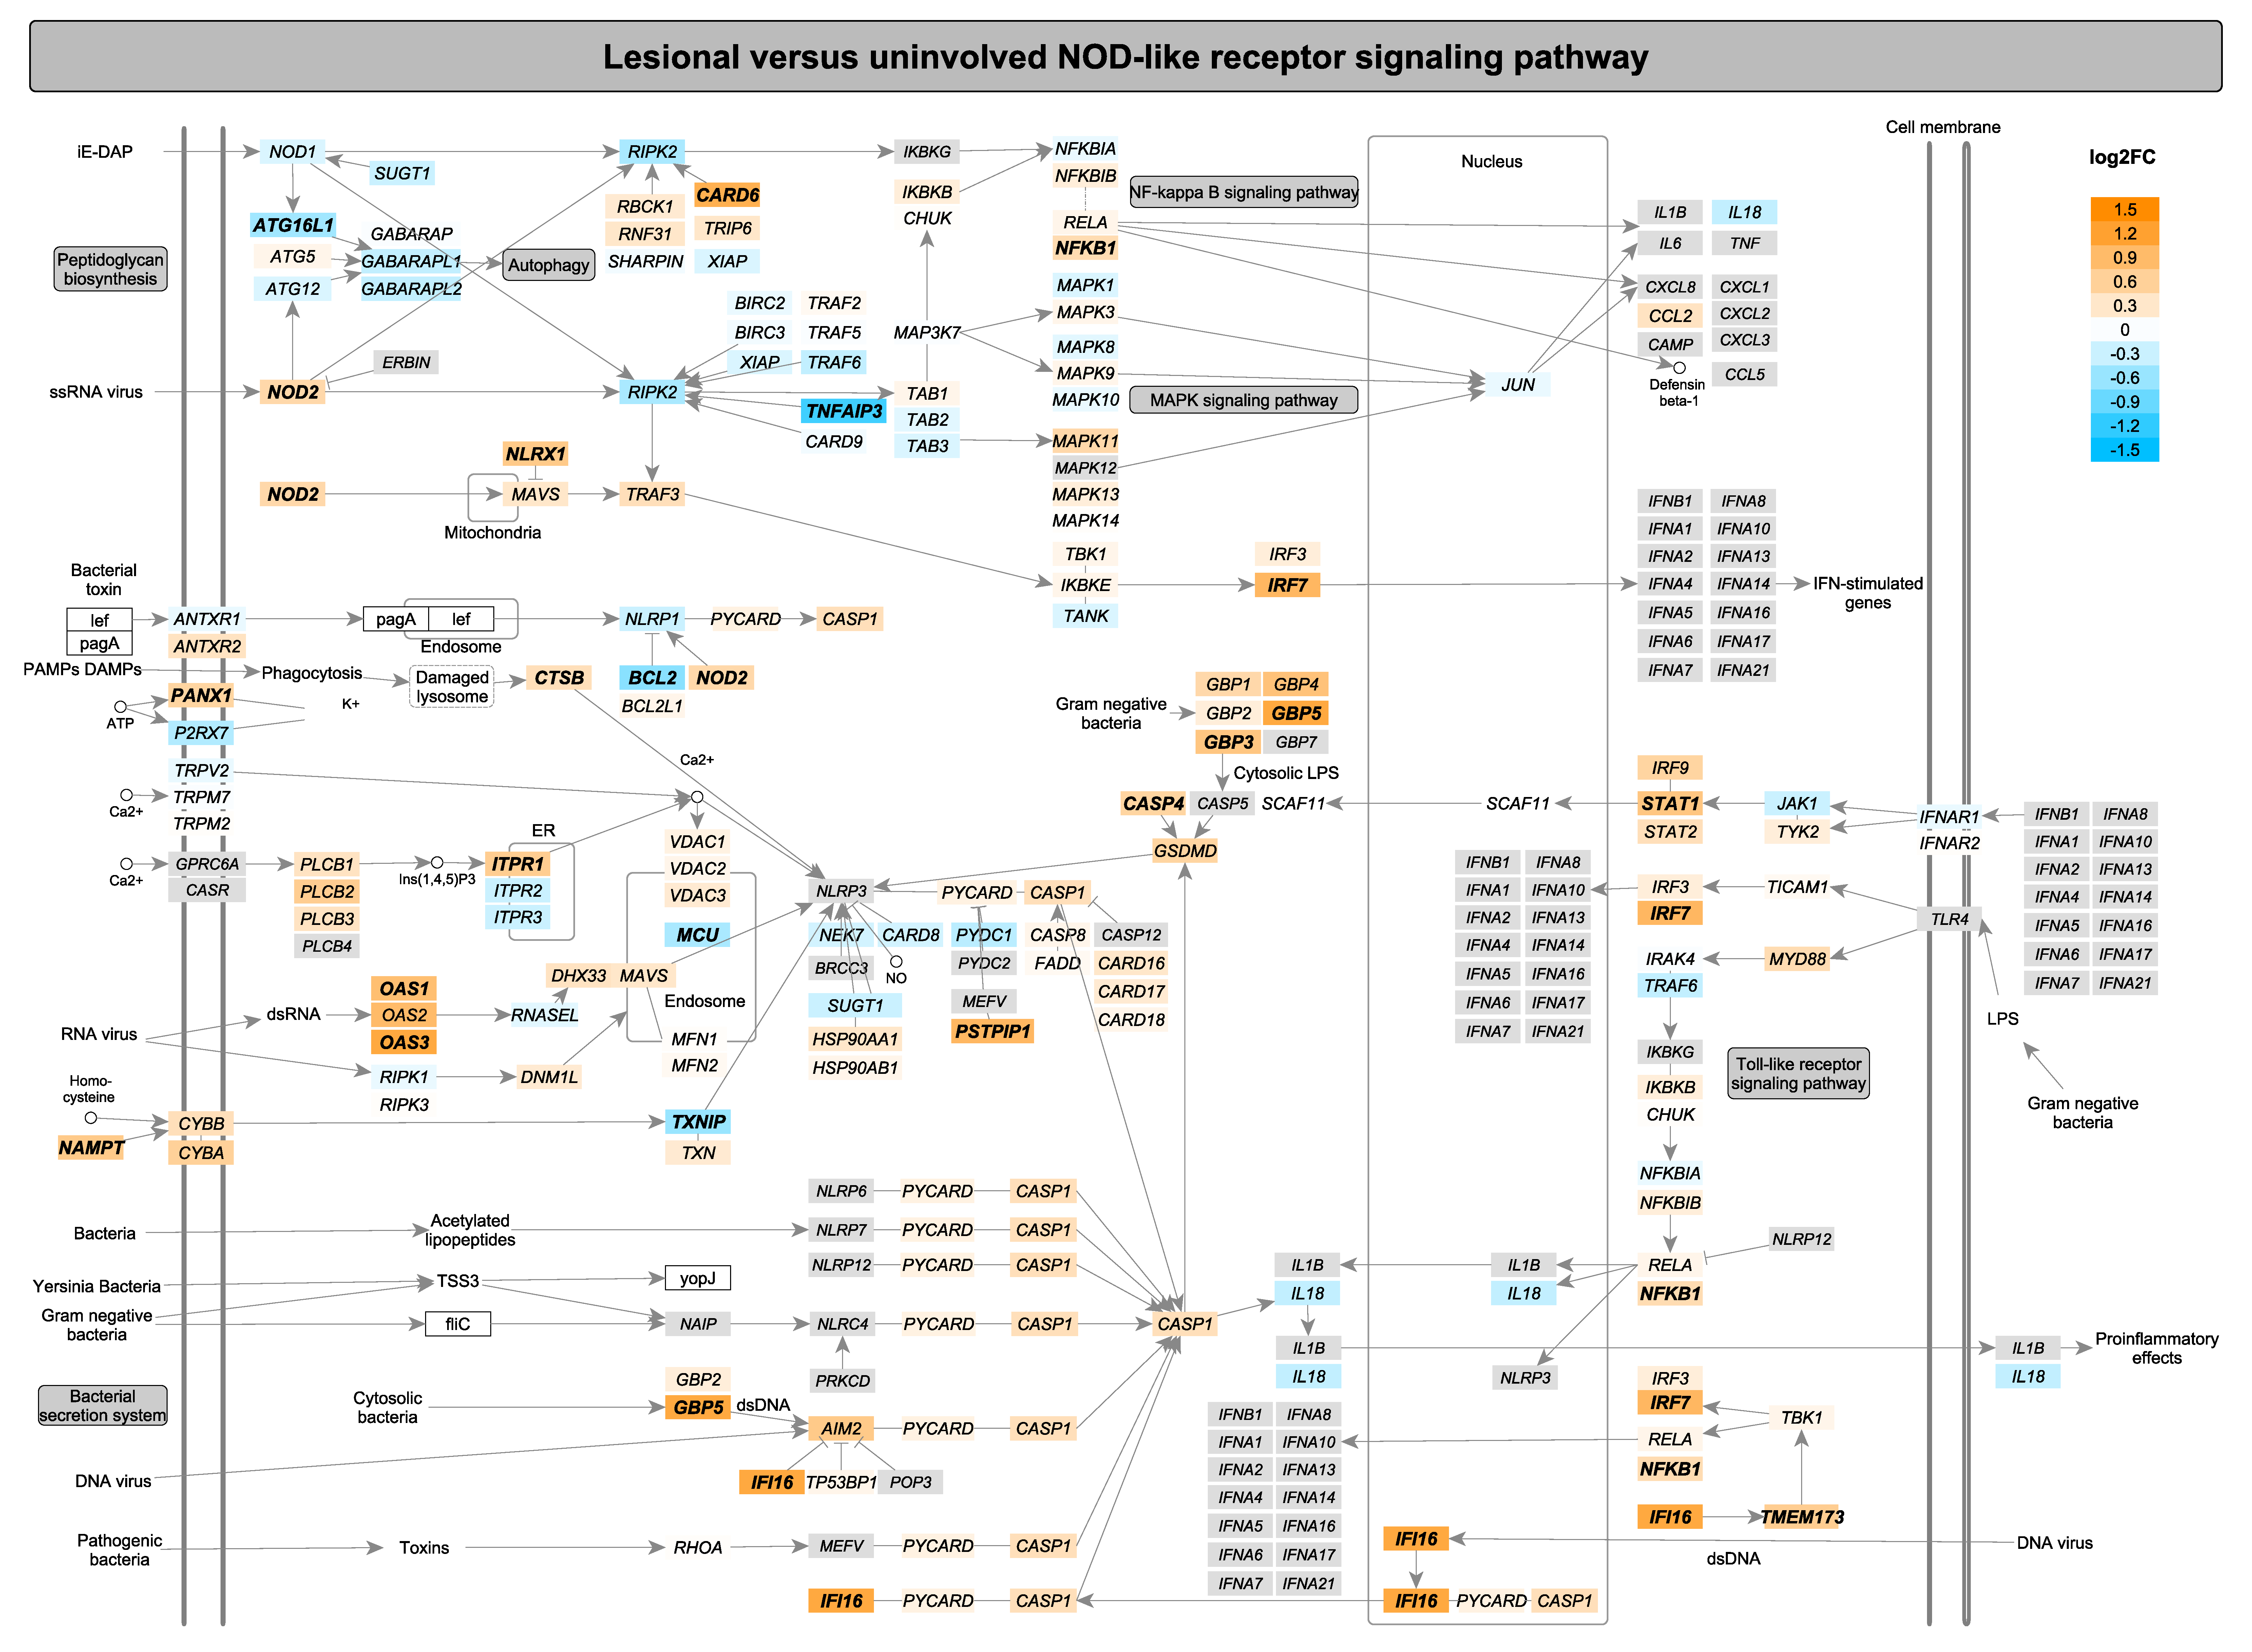
\includegraphics[width=\textwidth]{./Results2/pdfs/PS_lesional_uninvolved_all_NOD_like_pathway}
\caption[Mapping of the DEGs between lesional and uninvolved epidermis from psoriasis patients onto the NOD-like signalling pathway.]{\textbf{Mapping of the DEGs between lesional and uninvolved epidermis from psoriasis patients onto the NOD-like signalling pathway.} This pathway was sourced from KEGG, manually curated in a way that all member genes are maximised visually and then automatically color-coded by the log$_2$FC expression between the lesional and uninvolved epidermis. Significant DEGs (FDR$<$0.05) are highlighted in bold. This pathway was identified by pathway enrichment analysis using only DEGs (FDR$<$0.05).}
\label{figure:PS_lesional_vs_uninvolved_HIF_pathway}
\end{figure}
\end{landscape}


In addition to the NOD-I pathway, IL-17 signalling was another enriched pathway well known to be relevant in the development of psoriasis and the production of IL-17 by the Th-17 contributes to perpetuation of the innate host defense in the skin. Enrichment of the IL-17 signalling pathway in our data is driven by up-regulation of the S100 proteins family (\textit{S100A7}, \textit{S100A8} and \textit{S100A9}) and the chemokine \textit{CCL20}, which binds the CCR6 receptor and is involved in DCs and T cells chemotaxis. Moreover, enrichment of DEGs between lesional and uninvolved skin for the peroxisome proliferator-activated receptor (PPAR) signalling highlighted the link between metabolic dysregulation (particularly lipids) and innate immunity contributing to the psoriasis pathophysiology and increased risk of co-morbidities, such as metabolic syndrome and CVD. PPARs are ligand-dependent TF that have been shown to induce the inhibition of pro-inflammatory genes including IL-1 and TNF-$\alpha$ \parencite{Ji2001}. In skin, PPARs have been demonstrated to contribute to homeostasis by inducing differentiation and preventing proliferation \parencite{Rivier1998}. Moreover, inhibition of genes regulated by PPAR-$\gamma$ has been described in studies comparing lesional versus healthy skin biopsies \parencite{Li2014}.
%CCL20 https://www.ncbi.nlm.nih.gov/pubmed/19295614
%CCR6-CCL20 Dendritic Cells Rapidly Recruited into Epithelial Tissues via CCR6/CCL20 Are Responsible for CD8+ T Cell Crosspriming In Vivo

%Also sharing ECM, cell junctions and pathwsys in cancer, in our case microRNAs.

 

\subsection{Comparison of the systemic and tissue-specific gene expression signatures in psoriasis}
In order to commonalities and differences in psoriasis gene expression at the affected tissue (skin) and the systemic level (circulating immune cells), overlap between the different list of DEGs was performed. Only modest overlap was found between dysregulated genes in lesional skin compared to uninvolved and the DEGs identified in circulating immune cells, showing the greatest overlap CD14$^+$ monocytes and CD8$^+$ cells. Interestingly, a notable proportion of the overlapping DEGs presented opposite direction of change in circulating immune cells and in the skin from psoriasis patients. A relevant case is the \textit{TNFAIP3} gene, which was up-regulated in psoriasis CD4$+$ and CD8$^+$ cells compared to controls and down-regulated in lesional epidermis when compared to uninvolved.  In Tsoi \textit{et al.}, 2015 this gene did not change expression between nor between lesional and uninvolved or lesional and healthy skin and Li \textit{et al.}, reported its up-regulation in lesional skin. Another relevant trsnacript in the pathophysiology of psoriasis that presented opposite changes in CD$^+$ cells and in the skin analysis was the previously mentioned \textit{MIR146A}. This miRNA was also up-regulated in lesional skin when compared to healthy controls and seems to be a clear feature of psoriasis pathogenesis in the involved tissue.
 

\begin{table}[htbp]
%\setlength{\tabcolsep}{20pt} only to stretch the columns if you want
%\renewcommand{\arraystretch}{1.5}
\centering
\begin{tabular}{@{} c c c c}
\toprule
\textbf{DEGs overlapping}   & \textbf{Total overlap}   & \textbf{Same direction}  & \textbf{Opposite direction}\\
\textbf{with skin}          &                          &                          &                            \\
\midrule 
\midrule
CD14$^+$ monocytes          & 37                       & 19                       &  18                         \\ 
CD4$^+$                     & 10                       & 6                        &  4                           \\
CD8$^+$                     & 37                       & 24                       &  13                           \\
CD19$^+$                    & 16                       & 5                        &  11                          \\
\bottomrule 
\end{tabular}
\medskip %gap
\caption[Overlap of the dysregulated genes in the four circulating cell types (psoriasis patients versus controls) and the DEGs in psoriasis patients skin biopsies (lesional versus uninvolved).]{\textbf{Overlap of the dysregulated genes in the four circulating cell types (psoriasis patients versus controls) and the DEGs in psoriasis patients skin biopsies (lesional versus uninvolved). DEGs FDR$<$0.05 for each of the comparisons} }
\label{tab:RNAseq_overlap_circulating_versus_skin}
\end{table}
\bigskip %bigger spac


The limited overlap between circulating and skin DEGs was also reflected in the different enriched pathways identified for each analysis. The pathways enriched for CD14$^+$ and CD8$^+$ DEGs were mostly related to immune-related pathways, including TCR , IL-12 , TNF and NF-$\kappa$B signalling. Moreover, when compared to healthy controls, some of the genes in these circulating immune cells suggested certain immuno-supression features that could be characteristic of these cells before or/and after having been exposed to the skin inflammatory \textit{milieu}. The DEGs in lesional epidermis compared to uninvolved were enriched for pathways involved in metabolism, oxidative stress and cell cycle in addition to immune-related pathways. Moreover, the dysregulation of genes members of the immune-related pathways appeared to present an overall pro-inflammatory signature, reinforcing the differences between circulating immune cells and skin in the study of psoriasis pathophysiology.


\subsection{Integration of chromatin accessibility and expression data in circulating immune cells}
The characterisation of the chromatin accessibility landscape and the transcriptome in circulating immune cells from psoriasis patients, have revealed a greater effect of disease in gene expression than in chromatin accessibility. In order to assess to some extent the relationship between the two, overlap between DEGs and the genes proximal to a DARs ($\leq$5Kb) was performed. Limited overlap was only found CD8$^+$ cells, where 6  out of the 53 DARs were annotated by proximity to an RNA-seq DEGs in the same cell type (\textit{ARL4A},\textit{ASCL2}, \textit{ENTPD1}, \textit{TIAM1}, \textit{TRAT1} and \textit{ZNF276}). 

An interesting example is the T Cell lymphoma invasion and metastasis 1 (\textit{TIAM1}), which activates IL-17 expression and T cells transendothelial migration during inflammation \parencite{Kurdi2016, G\'{e}rard2009}. This gene showed an increased expression (log$_2$FC 0.44) in psoriasis patients CD8$^+$ cells (Figure \ref{figure:ATAC_RNAseq_CD8_TIAM1_combined} left). Likewise, psoriasis CD8$^+$ cells presented greater chromatin accessibility compared to healthy controls (log$_2$FC 0.41) in a region located at an intron of the \textit{TIAM1} gene and annotated as an active enhancer according to RoadMAp chromatin segmentation map for this cell type (Figure \ref{figure:ATAC_RNAseq_CD8_TIAM1_combined} right). Common SNPs within this peak did not appear to be an eQTL regulating expression of any gene in CD8$^+$ cells \parencite{Kasela2017} and chromatin conformation data did not reveal interaction of this particular region with the \textit{TIAM1} promoter \parencite{add}, difficulting the establishment of a mechanistic connection between chromatin accessibility and gene expression for this particular example in unstimulated conditions.



\begin{figure}[htbp]
\centering
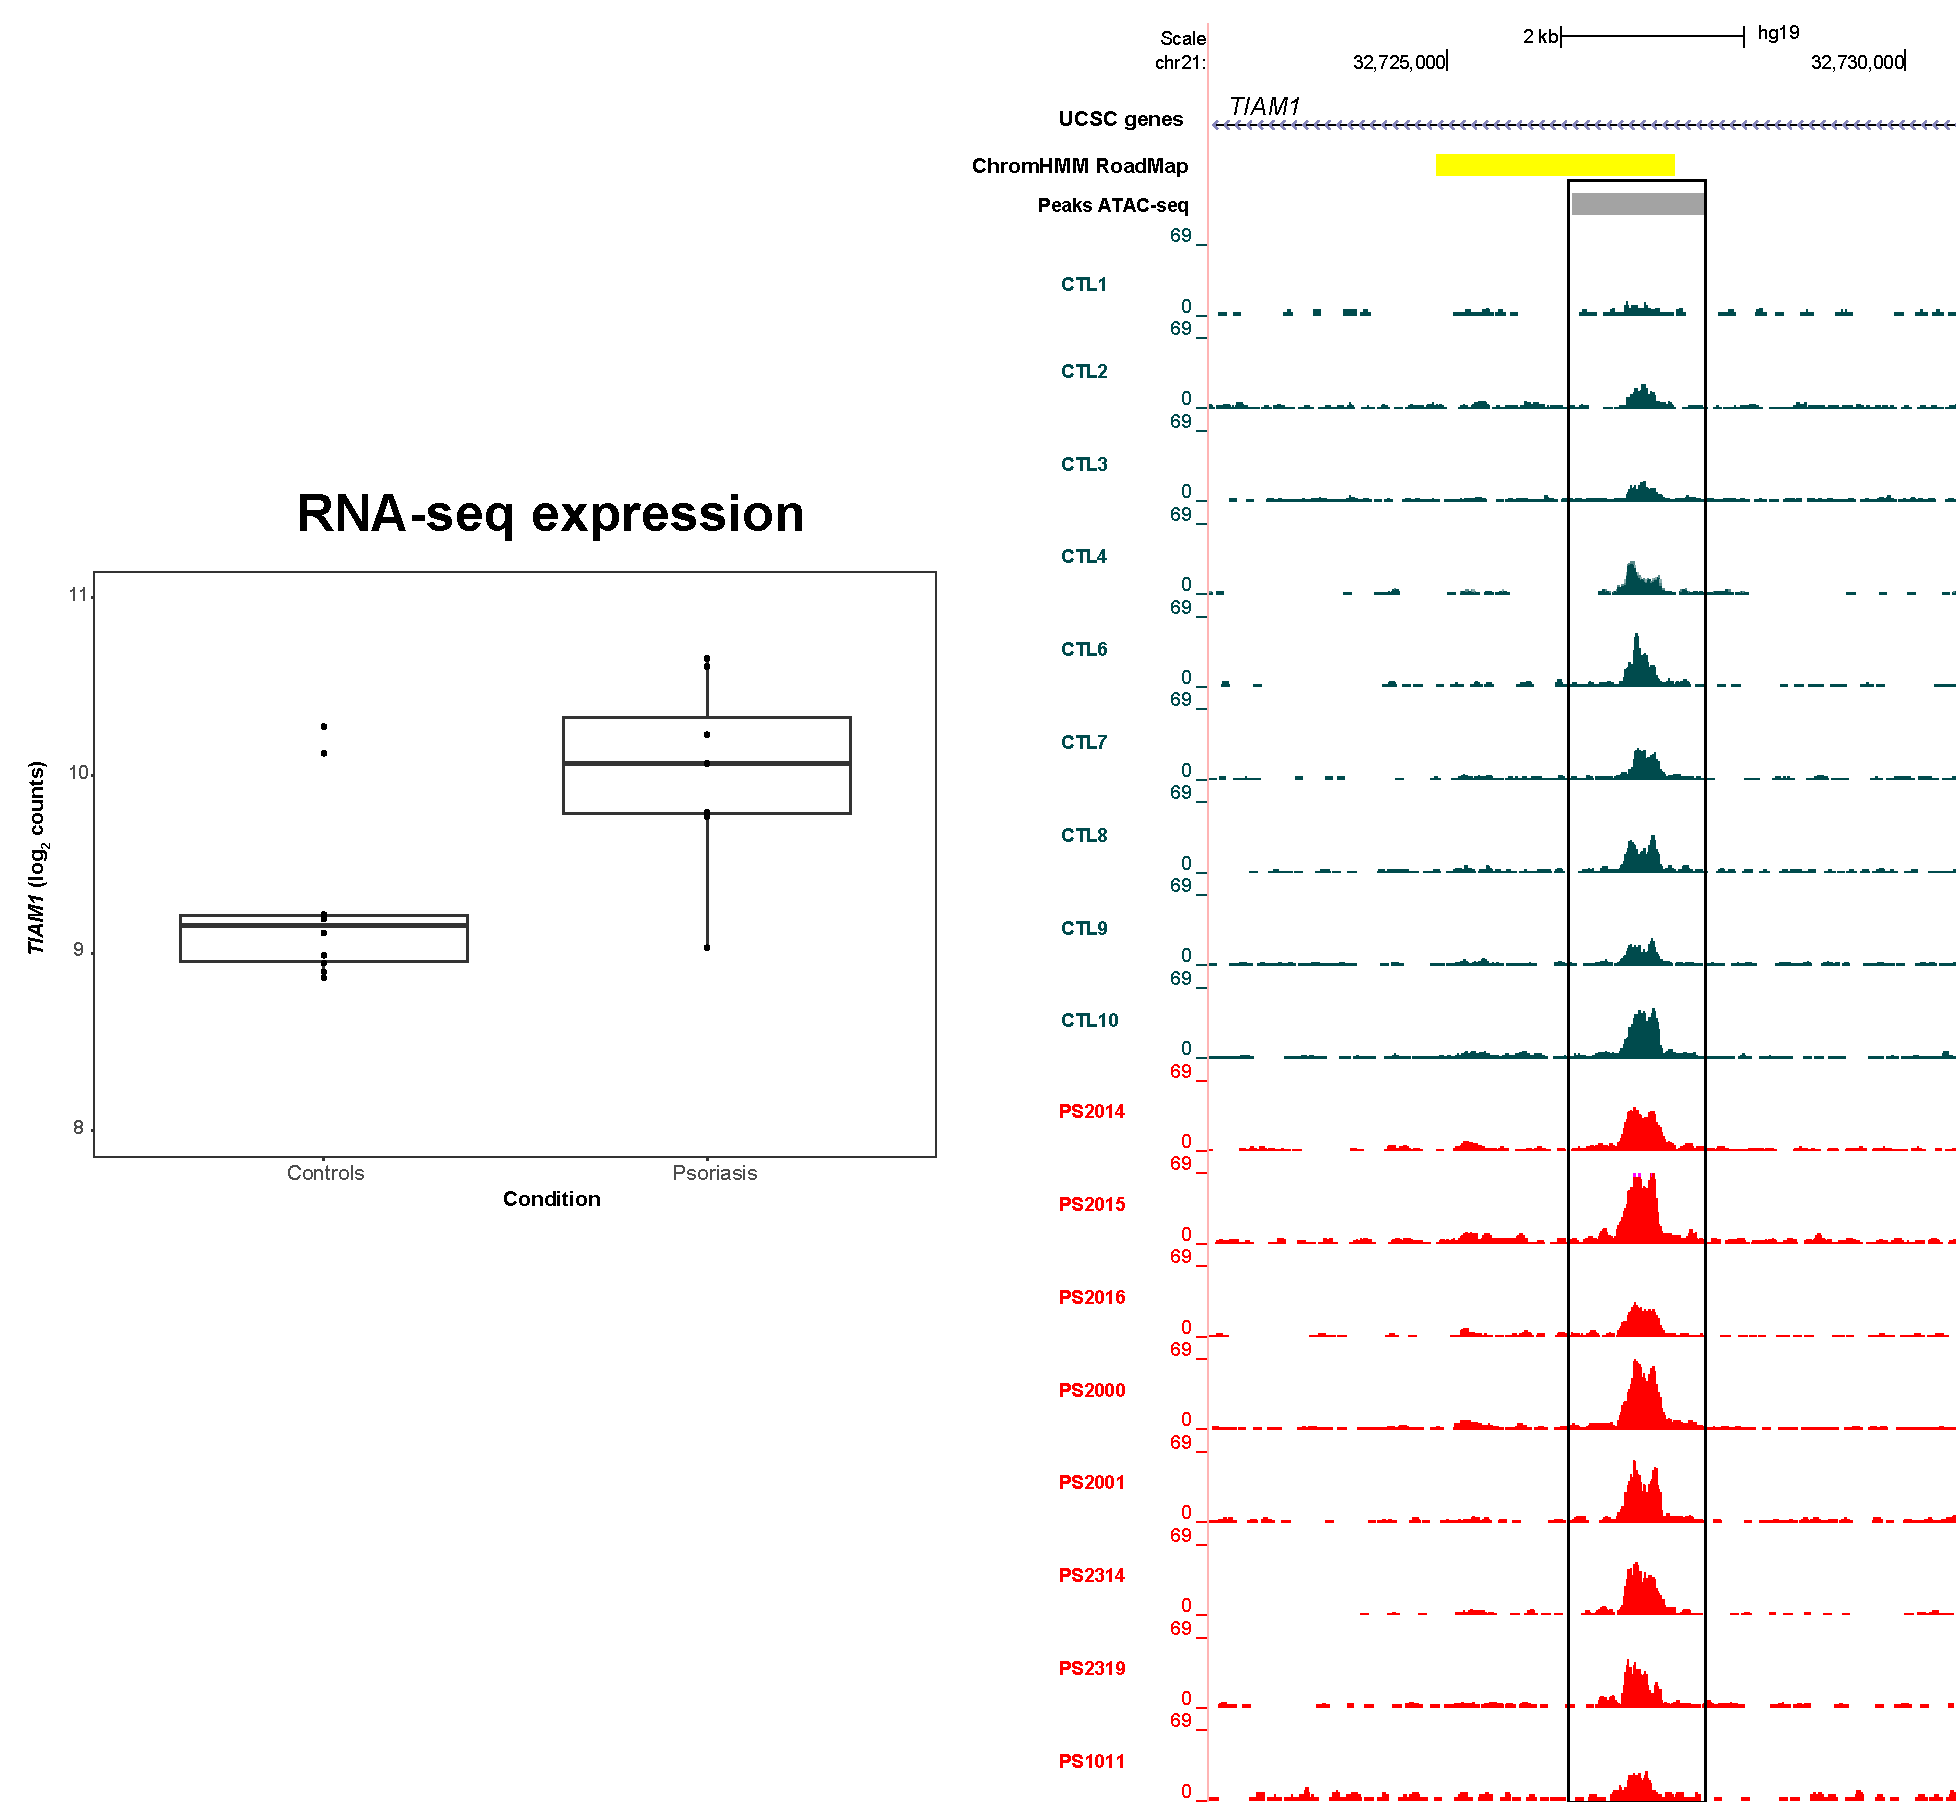
\includegraphics[width=0.8\textwidth]{./Results2/pdfs/ATAC_CD8_peak_TIAM1_RNA_combined}
\caption[Epigenetic landscape at the chr3:121,675,048-121,677,505 enhancer in circulating CD14$^+$ monocytes from psoriasis patients and healthy controls.]{\textbf{Epigenetic accessibility landscape at the chr3:121,675,048-121,677,505 enhancer in circulating CD14$^+$ monocytes from psoriasis patients and healthy controls.} Describe the track }
\label{figure:ATAC_RNAseq_CD8_TIAM1_combined}
\end{figure}



Another two relevant genes in the immune response for which ATAC-seq and RNA-seq presented overlap were the ectonucleoside triphosphate diphosphohydrolase 1 (\textit{ENTPD1}), which hydrolyses the pro-inflammatory mediator ATP attenuating the inflammation and acting as a modulator of the immune response, and the TCR-associated transmembrane adaptor 1 (\textit{TRAT1}) gene, a positive regulator of the TCR signalling \parencite{Antonioli2013, Valk2006}. Both genes presented up-regulated expression and an increased chromatin accessibility in psoriasis patients CD8$^+$ cells compared to healthy controls.

% mention about TIAM1 being a good target in Pi
%short check for the ENTPD1 and TRAT1 DARs to be likely to affect 
The changes in gene expression between psoriasis and healthy controls in the four circulating immune cell types included in this study have revealed a    

\subsection{Fine-mapping}



\subsection{Integration of GWAS fine-mapping results and functional data: locus 2p15}
\subsubsection{Maximising genetic commonalities across chronic inflammatory diseases}
The chr2p15 psoriasis risk locus (lead SNP rs10865331, OR=1.12) represents one of the GWAS associations located in a gene desert that was identified by the Immunochip study from Tsoi \textit{et al.},2012. This locus is shared with the chronic inflammatory diseases AS and CD. Interestingly, Reveille's AS GWAS study reported the same lead SNP as the psoriasis Immunochip \parencite{Reveille2010}. The later AS Immnochip study identified rs6759298 (OR=1.29) as the tag SNP for this region, which is in high LD (r$^2$=0.84) with rs10865331 \parencite{Cortes2012}. A recent GWAS meta-analysis combining five chronic inflammatory disease data, also identified association for the chr2p15 locus, confirming the same association and direction to be shared by the three phenotypes \parencite{Ellinghaus2016}. Therefore the AS and psoriasis associations are considered to be the same signal and likely to share the functional mechanism increasing the risk of a dysregulated inflammatory response.

As previously presented, fine-mapping using summary statistics from the psoriasis GAPC Immunochip cohort failed to successfully fine-map this locus (log$_10$BF<3). In contrast, genotype-based fine-mapping analysis performed in collaboration with Dr Anna Sanniti in the UK Immunochip AS data successfully identified an independent signal at chr2p15 (log$_10$BF 18.43) tagged by the SNP rs4672505. The refinement of this association signal in AS yielded a 95\% credible set containing only three SNPs. Out of the three identified SNPs, rs4672505 accounted for 40\% of the association in chr2p15 locus whereas the additional two SNPs (rs6759298 and rs6759003) explained together 60\% of this association. Interestingly, the SNP rs4672505 was also the lead SNP for the chr2p15 signal identified in the multi-disease meta-analysis from Ellinghaus and colleagues, previously mentioned \parencite{Ellinghaus2016}.

\subsubsection{Integration of ATAC and publicly available epigenetic data}
Rs4672505 was overlapping an accessible ATAC region included in the ML\_CD8 and not present in CD14$^+$ monocytes, tCD4$^+$ and CD19$^+$ cells (Figure UCSC track). The tCD8$^+$ accessible region harbouring rs4672505 was not a DARs between patients and controls and it appeared to have variability across individuals regardless disease status (Figure UCSC track with the CD8 only). 


\begin{figure}[htbp]
\centering
\begin{subfigure}{0.5\textwidth}
\centering
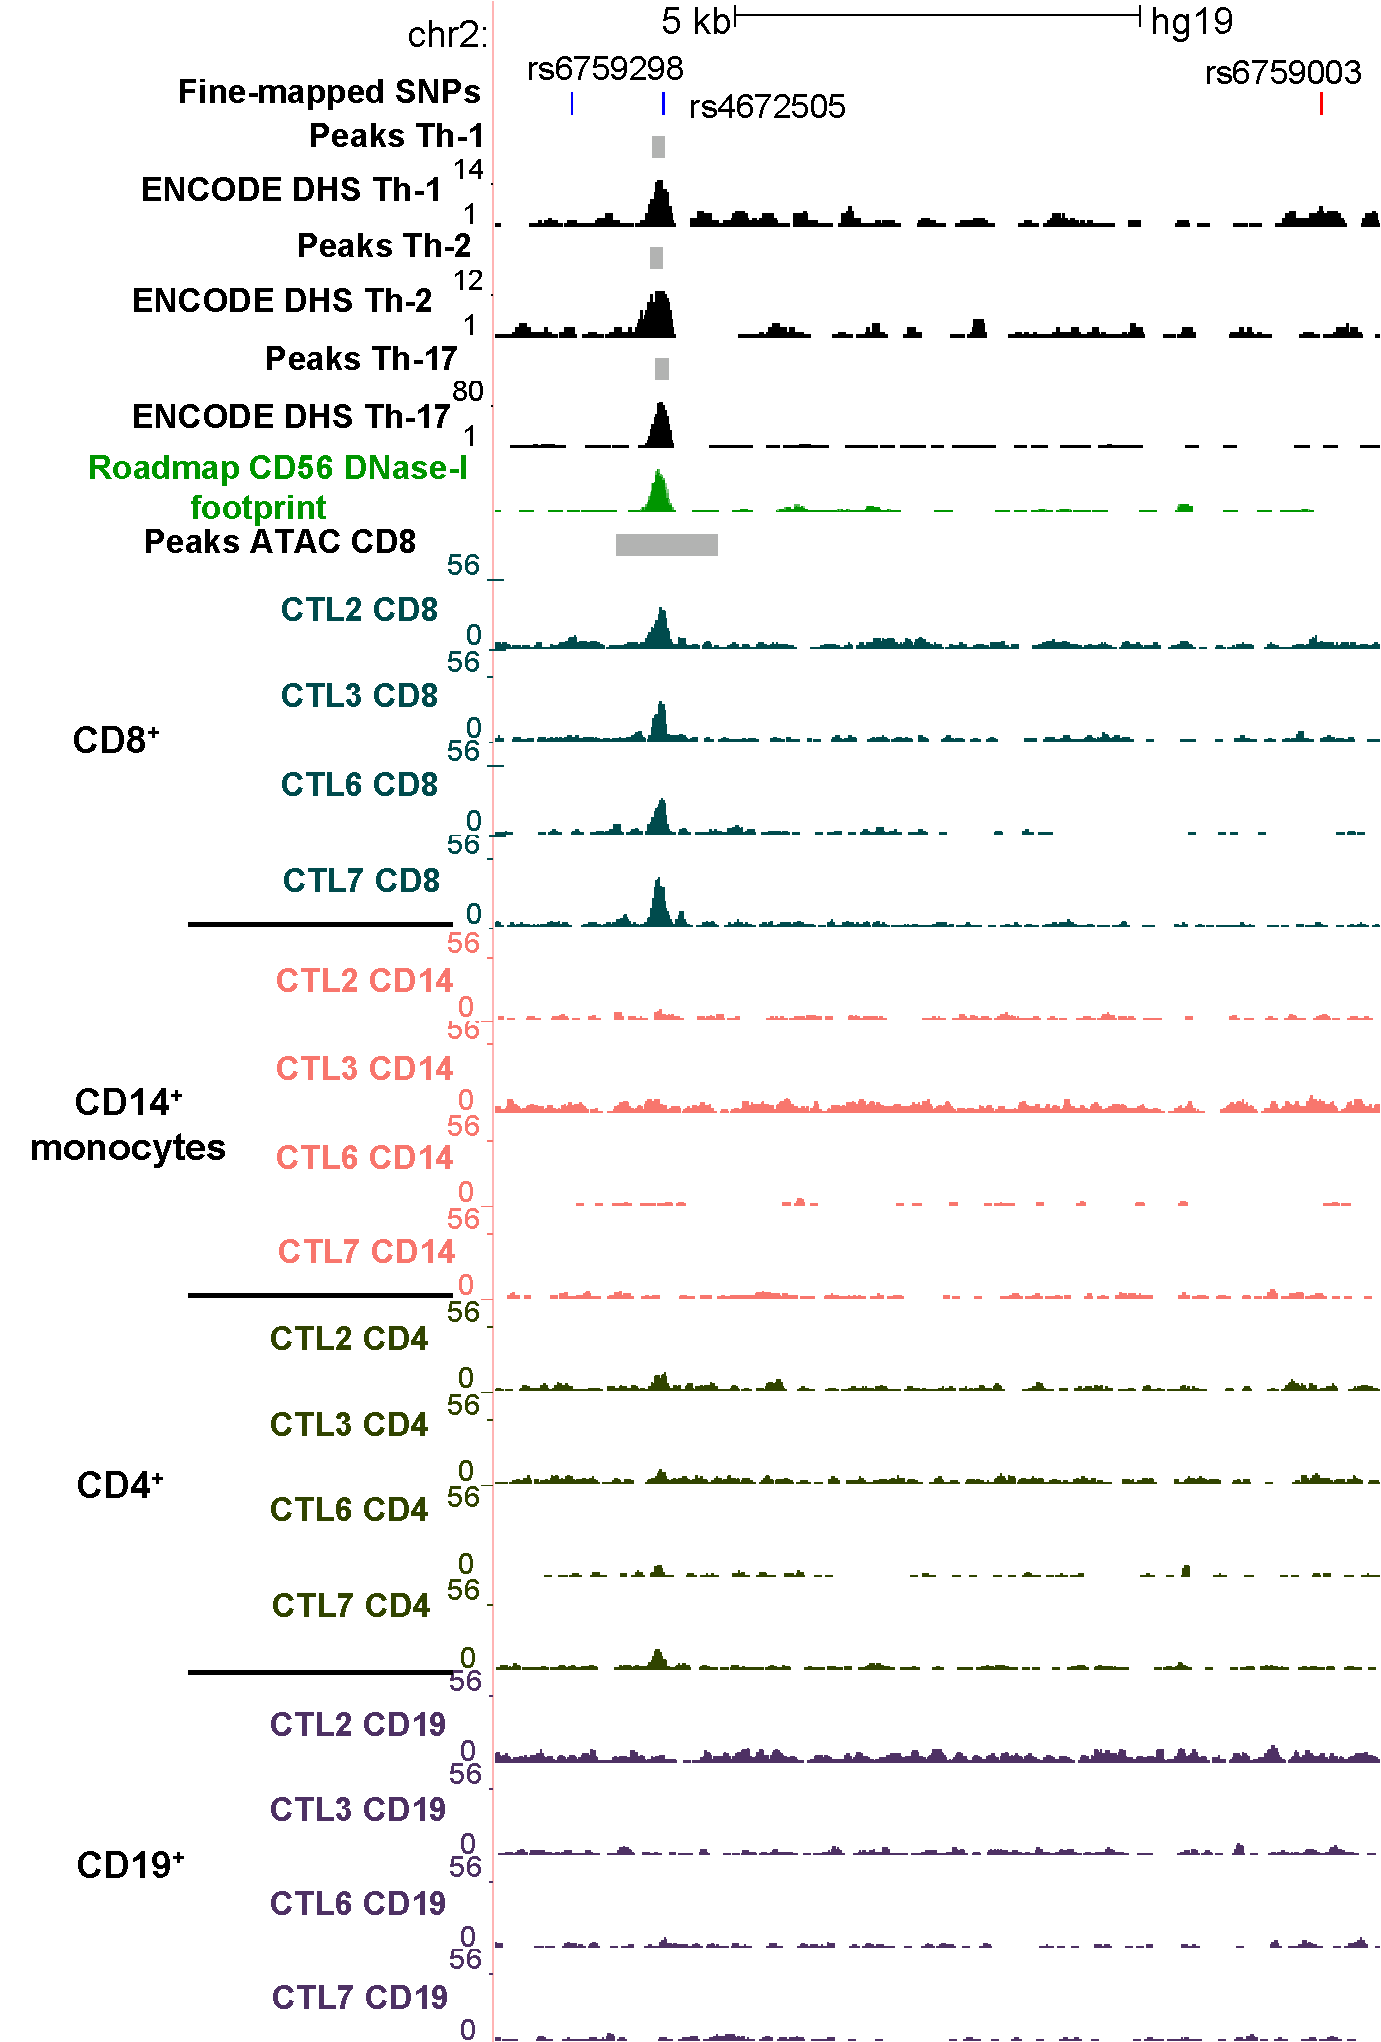
\includegraphics[width=\textwidth]{./Results2/pdfs/chr2p15_rs4672505_FM_all_cell_types_track_all_marks}
\caption{\textbf{}}
% The percentage sign indicated that the other subfig goes side by side
\end{subfigure}%
\begin{subfigure}{0.5\textwidth}
\centering
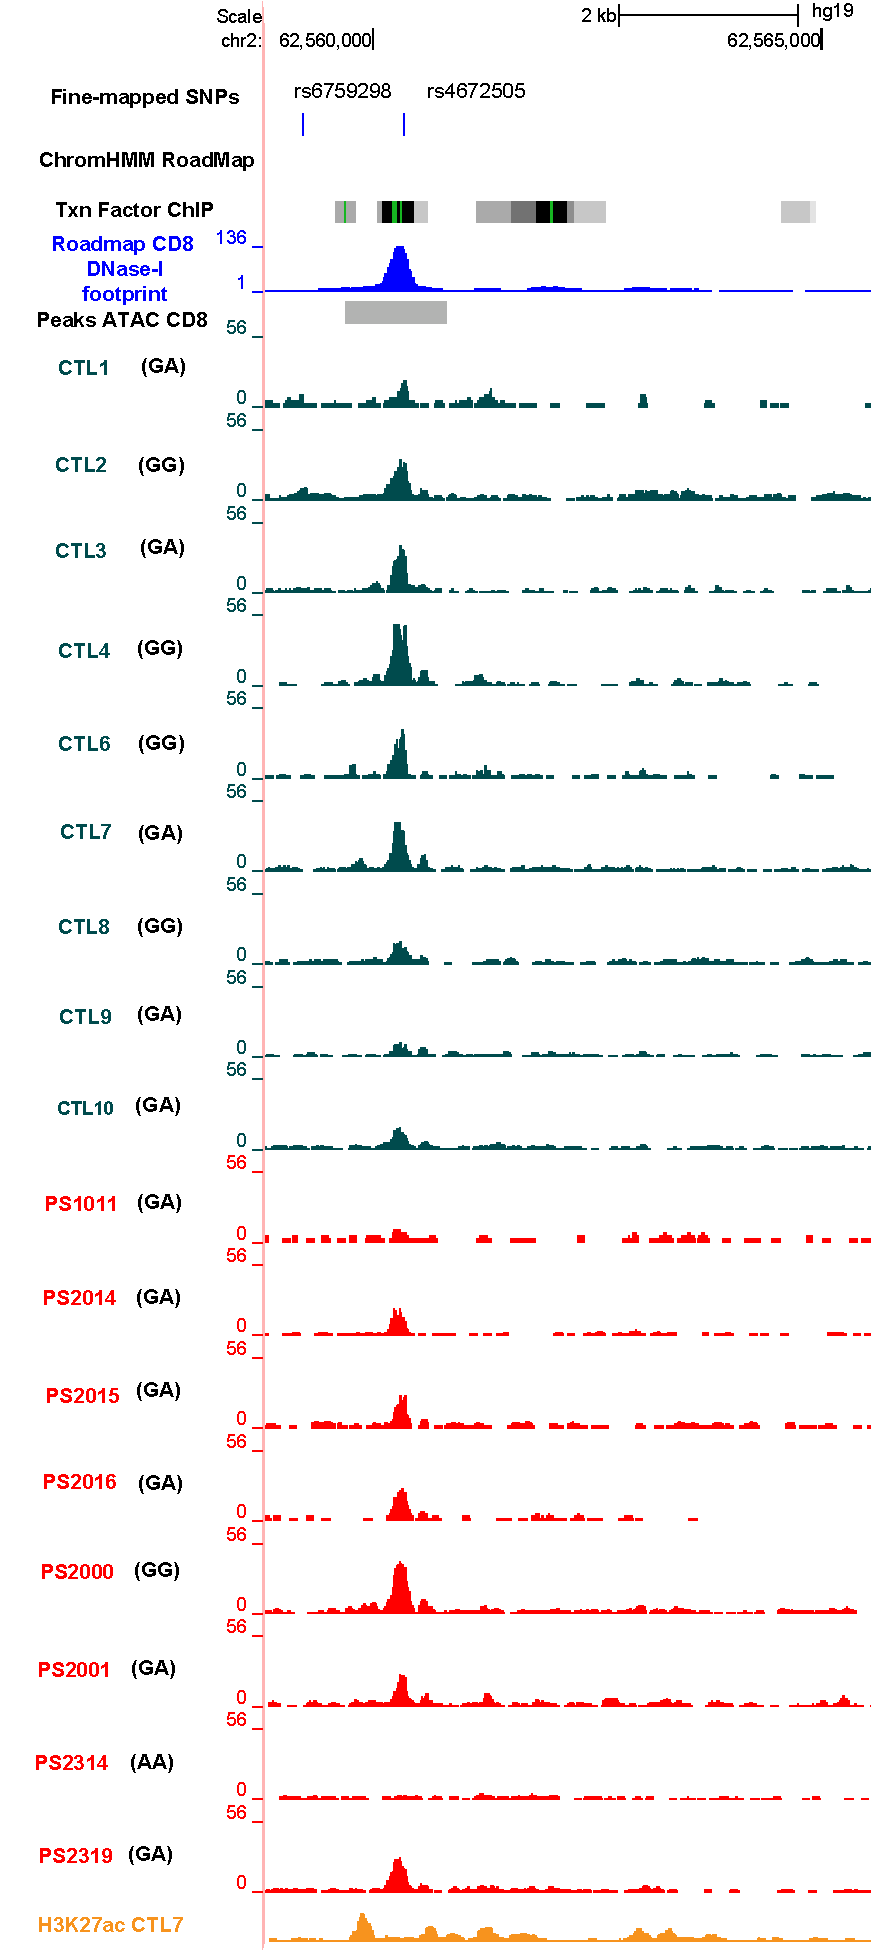
\includegraphics[width=\textwidth]{./Results2/pdfs/chr2p15_rs4672505_FM_CD8_track_all_marks}
\caption{\textbf{}}
\end{subfigure}
\caption[Epigenetic landscape at the chr2p15 locus.]{\textbf{Epigenetic landscape at the chr2p15 locus.}Mention the genotype by Sanger sequencing is included for each of the samples}
\label{figure:ATAC_PS_CTL_chr2p15_rs4672505}
\end{figure} 


For example, PS1011 and CTL1 showed no ATAc signal at this location when compared to PS2000 and CTL4. Integration with publicly available DHS data also revealed accessible chromatin at rs4672505 in Th-1, Th-2 and Th-17 cells from ENCODE (Figure UCSC track). Although this region was tagged as quiescent according to the tCD8$^+$ chromatin segmentation, Epigenome Roadmap primary tCD8$^+$ DNase-I digital genomic footprinting signal was found to overlap with rs4672505 and the in-house ATAC peak (Track), and may indicate genomic locations with \textit{cis}-regulatory roles. The absence of histone marks and chromatin accessibility leading to annotation of this chromatin segment as quiescent by the Epigenome Roadmap could be explained by the variability across individuals found at this region. Regarding TFs, ENCODE ChIP-seq experimental data from GM12878 showed binding for RUNX3, a psoriasis and AS GWAS associated gene, which also showed nominal association in the PsA Immunochip GWAS study. Importantly, RUNX3 is together with a number of TFs involved in CD8$^+$ cells differentiation \parencite{Wong2011}  Further investigation using \textit{in silico} TFBS prediction, such as PROMO \parencite{Messeguer2002}, and ENCODE genomic DNase-I footprint in GM128778 predicted STAT1 binding at rs4672505. Future experimental work will be required to confirm these observations. Altogether, integration of ATAC and publicly available epigenetic indicated that rs4672505 was the most likely variant, amongst the three fine-mapped SNPs included in the 95\% credible set, to have a functional role explaining the association of chr2p15 with psoriasis risk.

% Not sure where to include the methyl QTLs

\subsubsection{Allele-dependent chromatin accessibility and allelic imbalance using ATAC reads at rs4672505}
In order to investigate the role of rs4672505 in the variability of chromatin accessibility across individuals in this region, Sanger sequencing was performed to determine the genotype for each of the individuals. Amongst the eighteen samples (ten controls and eight psoriasis patients), one (PS2314) was homozygous for the risk allele (A, MAF=0.43), eleven were heterozygous and six were homozygous for the protective allele (G). Interestingly, PS2314, the only homozygous individual for the risk allele showed complete absence of the peak at rs4672505. The normalised read counts were retrieved at the chr2:62,559,749-62,561,442 ML\_CD8 peak and used as dependent variable to perform linear model analysis based on rs4672505 genotype using batch as a covariate. 



\begin{figure}[htbp]
\centering
\begin{subfigure}{0.5\textwidth}
\centering
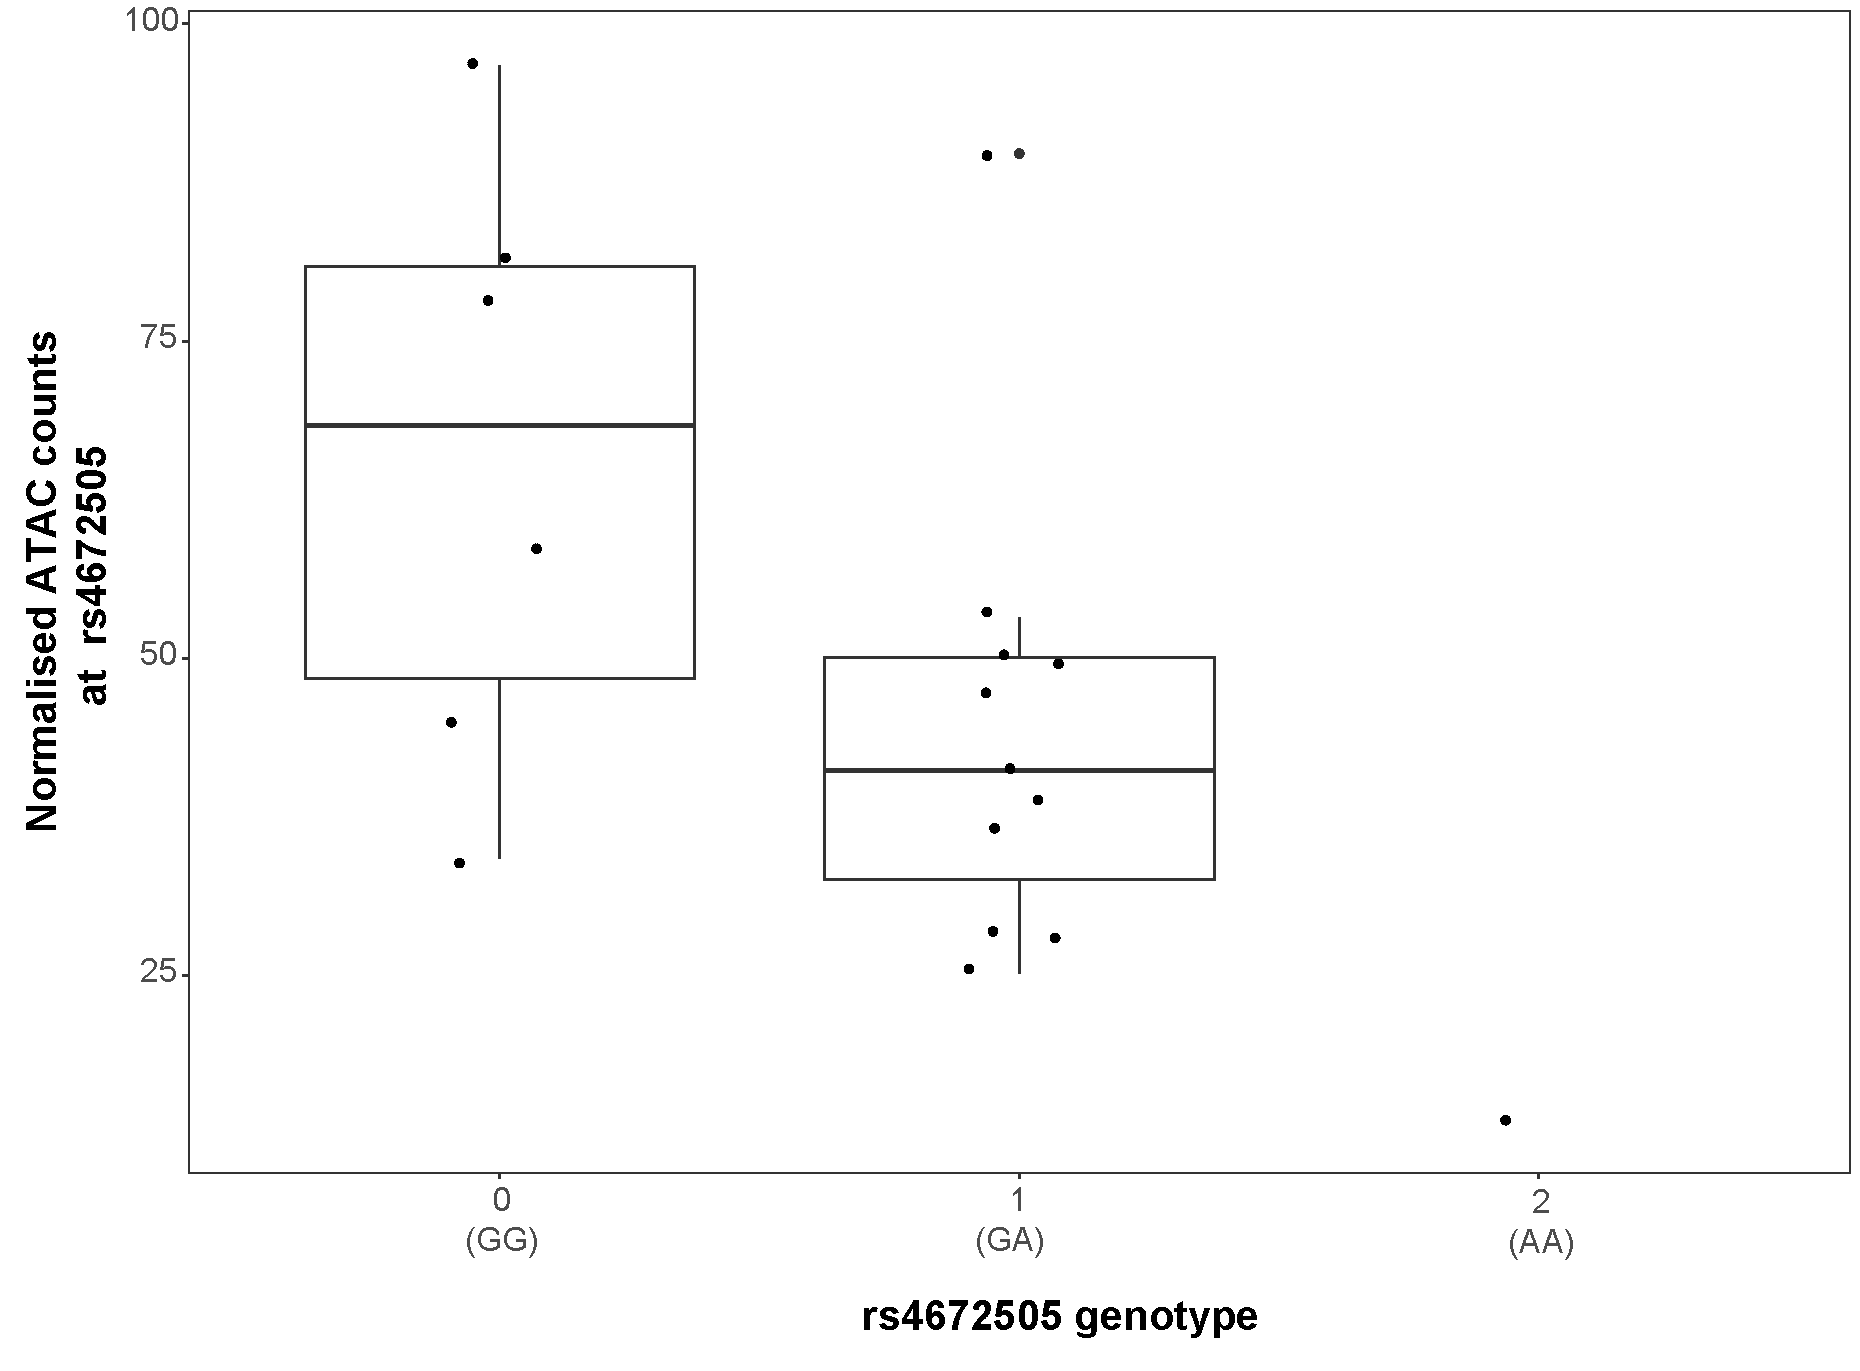
\includegraphics[width=\textwidth]{./Results2/pdfs/ATAC_caQTL_CD8_final}
\caption{\textbf{}}
% The percentage sign indicated that the other subfig goes side by side
\end{subfigure}%
\begin{subfigure}{0.5\textwidth}
\centering
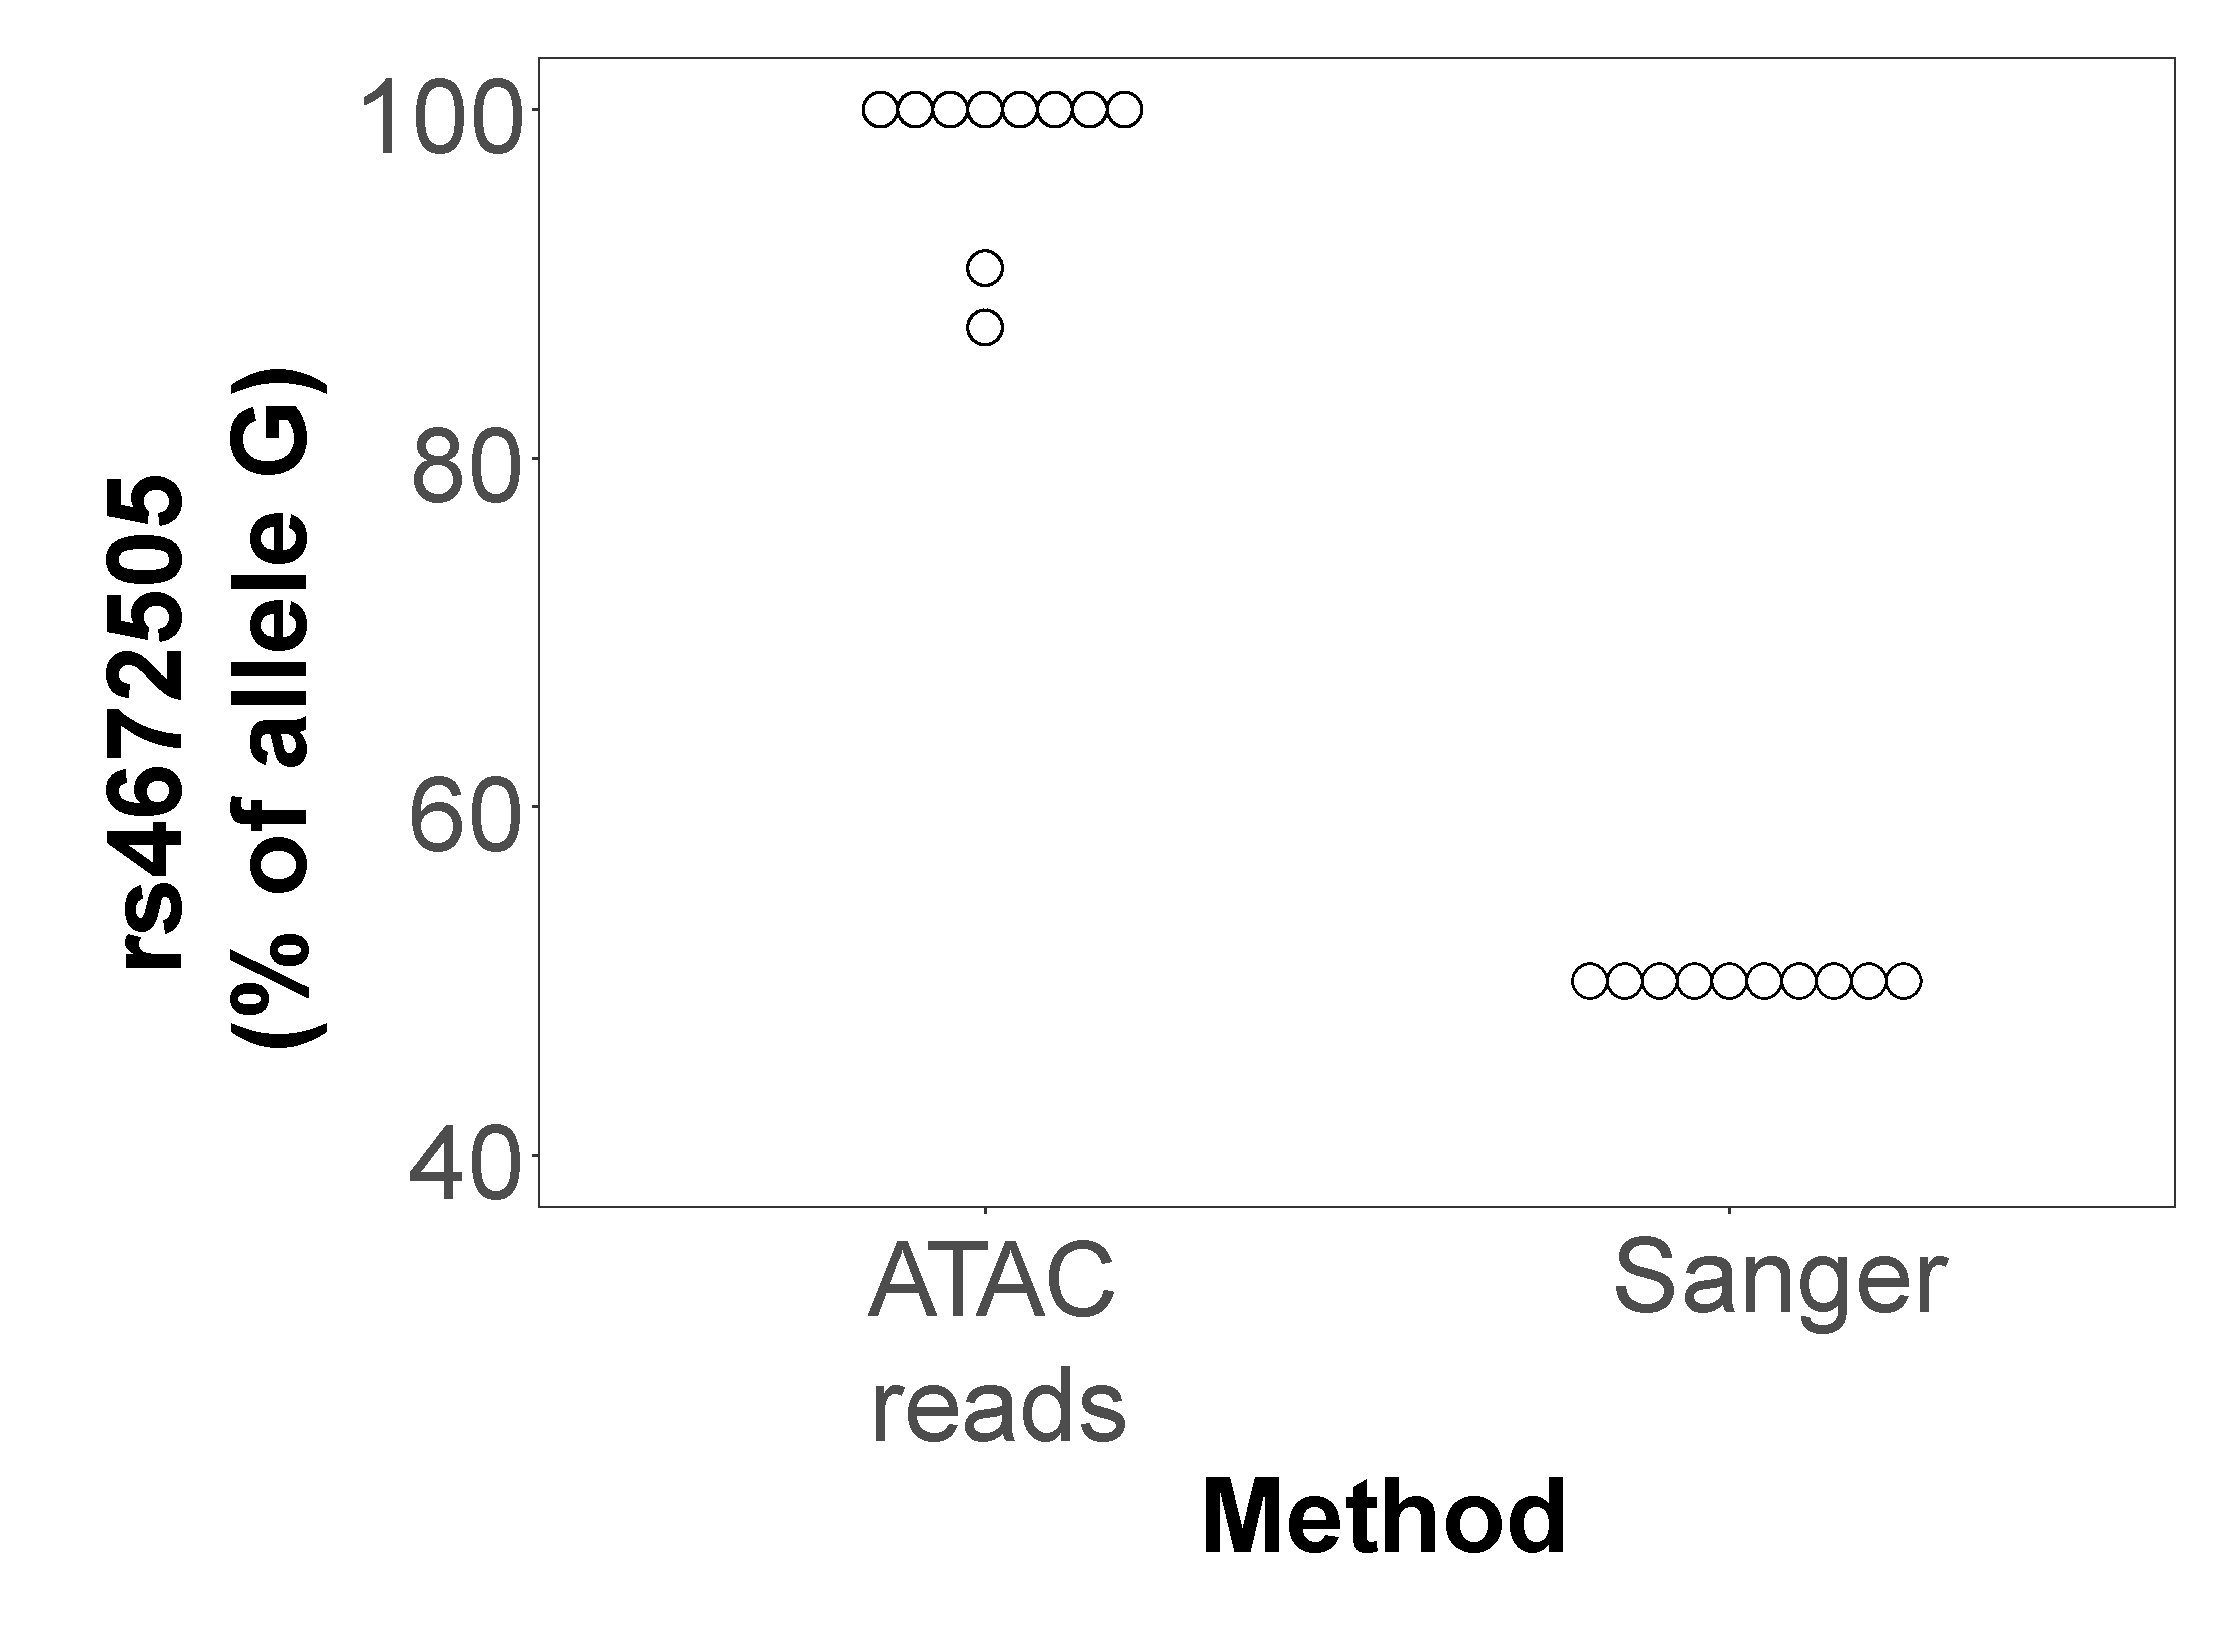
\includegraphics[width=\textwidth]{./Results2/pdfs/chr2p15_rs4672505_allelic_imbalance_CD8_final}
\caption{\textbf{}}
\end{subfigure}
\caption[Mapping rate and total reads after filtering (million) mapping to Ensembl genes in all the RNA-seq samples from psoriasis patients and controls in four cell types.]{\textbf{Mapping rate and total reads after filtering (million) mapping to Ensembl genes in all the RNA-seq samples from psoriasis patients and controls in four cell types.} a) The mapping rate refers to the percentage of total sequenced reads from each sample that uniquely mapped to a particular site of the genome. b) The total number of reads after filtering for non-uniquely mapped and duplicated reads that mapped to Ensembl features, including coding protein genes and lncRNAs.}
\label{figure:ATAC_PS_CTL_caQTL_and_allelic_imbalance}
\end{figure} 






Significant negative correlation (pval=0.035) was found, suggesting allele-dependent chromatin accessibility. Furthermore, ATAC reads allelic imbalance was investigated at rs4672505 position on those individuals identified as heterozygous by Sanger sequencing. This analysis demonstrated a larger percentage of ATAC reads (greater than the expected 50\%) preferentially tagging the protective allele G and were not driven by mapping bias, since A was the reference allele in the hg19 build used to map the ATAC data. Overall, these results showed a tendency towards greater chromatin accessibility in presence of the fine-mapped protective allele at the chr2p15 psoriasis GWAS locus.
 

\subsubsection{Potential regulatory role of rs4672505 in the expression of B3GNT2}

Public eQTL in blood but not in CD4 and CD8
My RNA-seq data at that locus



%%%%%%%%%%%%%%%%%%%%%%%%%%%%%%%%%%%%%%%%%%%%%%%%%%
\section{Discussion}

% Lack of H3K27ac
%Enrichment of trait associated variants within chromatin marks
Trynka papers talking about relevant histone marks and similar studies. may be because is not one of the histones presenting phenotypic cell type specificity for complex disease GWAS SNPs and also in Lin did not appear as one of the histone marks that presented changes across the different cell types.

%Code and Lee did not show overlap at all between them
% Discrepancies with Code and Lee Nevertheless, the fundamental differences between our study and the other two aforementioned studies together with the differences in the platform to test measure gene expression may explain the lack of overlap.
% T cell study from Palau is interesting from the point of view of similar pathway and some of them common to skin that could indicate that the circulating genes have a similar dysregulation just in a different direction
%IL-10 paper Jung is very interesting because it shows some differences in terms of some pro-inflammatory genes that were also down in the monocytes at the first point of stimulation that has been already said was not the one when all the genes expression of relevant genes changes, but could give a closer scenario for comparison with our study. However the severity of disease (PASI mean is 27) may also drive some of the differences together with the technology


% Reported pathways in the PBMCs studies:
	% Coda: DEGs in blood were not enriched for any GO term. However 15 DEGs were member from immune system functions, 9 genes assciated with lipid and fatty acid metabolism, 10 with apoptosis and 9 with proteolysis, 9 with oxidation-reduction and 6 as oxidative stress
	% Lee: no pathway analysis but hints about IL7R over-expression and also about reduced expression of NFkB inhibitors such as IkB which points towards over-activation of the NFkB as well as also changes in cell cycle related to greater proliferation and differences in cell cycle progression
	%Mesko:no differences in IFNG or other more IFN related genes in PBMCs. Functional characterisation of DEGs in psoriasis mainly pointed towards response to external stimuli, followed by unclasified and cell growth and maintenance
	% Palau: T cell activation and DEGsbetween activated psoriasis and patients T cellsIFN signalling, IL12-STAT4 pathways (which is an IFNG induced pathway), RIG-I pathwayand the NLR family of receptors like NOD2 overall suggesting greater IFN activation in the patients T cells. Also a set of genes associated to viral infection response (similar finding in skin)
	%Jung can be useful for particular examples of pro-inflammatory genes down-reg in patients


%Paper:Macrophage-derived cytokine and nuclear factor kappaB p65 expression in synovial membrane and skin of patients with psoriatic arthritis.



Skin other studies Swindell
%The study from \parencite{Swindell2017} investigating the changes between psoriasis and normal skin in cultures of epidermal KCs and whole biopsies represented the most similar approach to the one adopted here. Due to the lack of global publicly available results for this study, a limited comparison was performed focusing in some of the results including in the manuscript. Consistently with our results, Swindell and colleagues also detected a similar proportion of up- and down-regulated genes between lesional and uninvolved KCs in culture (63 and 83 genes, respectively). However, the number of dysregulated genes identified in the cultured epidermal KCs was notably lower when compared to our approach of epidermis layers without culture. Swindell study identified the top 24 genes modulated between lesional and uninvolved cultured KCs with the greatest dissimilarity in change when performing the same analysis using whole biopsies. Amongst those only three presented to be significantly dysregulated between lesional and uninvolved epidermis in our data (\textit{UGT3A2}, \textit{SNTB1} and \textit{SERPINB2}). \textit{UGT3A2} was up-regulated in the cultured KCs comparison and not differentially expressed when using whole biopsies in Swindell's study. Conversely, our data showed down-regulation of \textit{UGT3A2}. For \textit{SNTB1} and \textit{SERPINB2}, the down-regulation in Swindell data was consistent with our results. 


%Amongst the genes that Swindell and colleagues demonstrated to have opposite patterns of expression when comparing lesional and normal skin in cultured KCs or whole biopsies were proteins from the S100 family, including S100A8 and S100A9. Particularly, these two members of this family have been identified to be pro-inflammatory and up-regulated psoriasis lesional skin, suggesting that cell culture may be having a confounding effect in regulating gene expression \parencite{Ryckman2003}. Regarding expression of early KC differentiation genes, Swindell reported significant down-regulation of \textit{KRT1} and \textit{DSC1} in lesional skin when compared to uninvolved in cultured KCs. In contrast, our data failed to show dysregulation of these two genes between lesional and uninvolved epidermis, similarly to the observation when comparing whole biopsies in Swindell's data. This may indicate that dysregulation of early and late KC differentiation genes between lesional and uninvolved skin may be missed in absence of the cell culture stimuli when using either epidermis sheets or whole punch biopsies.   

%Why our results more similar to Tsoi than the epidermis biopsies: This could be partly to the use of standard RNA-seq methods and a paired-analysis in Tsoi \textit{et al.} 2015 and our study
 
skin and sf comparison
https://www.ncbi.nlm.nih.gov/pmc/articles/PMC4406155/
%The relevance of circulating immune cells in the initiation and termination of psoriasis has been demonstrated in report cases studies of patients undergoing bone-marrow transplantation \parencite{Eedy1990, Gardembas1990}.
%Gupta2016 normal and lesional skin pre and post treatment	RNA-seq
%In terms of personalised epigenome studies in psoriasis, a epigenomic-wide association study (EWAS) investigating DNA methylation has been conducted \parencite{Zhou2016}. Interestingly, this study revealed nine disease-associated differentially methylated sites underlying disease status and environmental factors but no overlap with genetic effects.
%Future plans: Importantly, Hi-C combined with H3K27ac ChIP has also allowed to identify specific enhancer$–$promoter interactions in primary human cells \parencite{Mumbach2017}.